\documentclass[twoside]{book}

% Packages required by doxygen
\usepackage{calc}
\usepackage{doxygen}
\usepackage{graphicx}
\usepackage[utf8]{inputenc}
\usepackage{makeidx}
\usepackage{multicol}
\usepackage{multirow}
\usepackage{textcomp}
\usepackage[table]{xcolor}

% Font selection
\usepackage[T1]{fontenc}
\usepackage{mathptmx}
\usepackage[scaled=.90]{helvet}
\usepackage{courier}
\usepackage{amssymb}
\usepackage{sectsty}
\renewcommand{\familydefault}{\sfdefault}
\allsectionsfont{%
  \fontseries{bc}\selectfont%
  \color{darkgray}%
}
\renewcommand{\DoxyLabelFont}{%
  \fontseries{bc}\selectfont%
  \color{darkgray}%
}

% Page & text layout
\usepackage{geometry}
\geometry{%
  a4paper,%
  top=2.5cm,%
  bottom=2.5cm,%
  left=2.5cm,%
  right=2.5cm%
}
\tolerance=750
\hfuzz=15pt
\hbadness=750
\setlength{\emergencystretch}{15pt}
\setlength{\parindent}{0cm}
\setlength{\parskip}{0.2cm}
\makeatletter
\renewcommand{\paragraph}{%
  \@startsection{paragraph}{4}{0ex}{-1.0ex}{1.0ex}{%
    \normalfont\normalsize\bfseries\SS@parafont%
  }%
}
\renewcommand{\subparagraph}{%
  \@startsection{subparagraph}{5}{0ex}{-1.0ex}{1.0ex}{%
    \normalfont\normalsize\bfseries\SS@subparafont%
  }%
}
\makeatother

% Headers & footers
\usepackage{fancyhdr}
\pagestyle{fancyplain}
\fancyhead[LE]{\fancyplain{}{\bfseries\thepage}}
\fancyhead[CE]{\fancyplain{}{}}
\fancyhead[RE]{\fancyplain{}{\bfseries\leftmark}}
\fancyhead[LO]{\fancyplain{}{\bfseries\rightmark}}
\fancyhead[CO]{\fancyplain{}{}}
\fancyhead[RO]{\fancyplain{}{\bfseries\thepage}}
\fancyfoot[LE]{\fancyplain{}{}}
\fancyfoot[CE]{\fancyplain{}{}}
\fancyfoot[RE]{\fancyplain{}{\bfseries\scriptsize Generated on Sun Nov 27 2016 13\-:24\-:42 for tonav by Doxygen }}
\fancyfoot[LO]{\fancyplain{}{\bfseries\scriptsize Generated on Sun Nov 27 2016 13\-:24\-:42 for tonav by Doxygen }}
\fancyfoot[CO]{\fancyplain{}{}}
\fancyfoot[RO]{\fancyplain{}{}}
\renewcommand{\footrulewidth}{0.4pt}
\renewcommand{\chaptermark}[1]{%
  \markboth{#1}{}%
}
\renewcommand{\sectionmark}[1]{%
  \markright{\thesection\ #1}%
}

% Indices & bibliography
\usepackage{natbib}
\usepackage[titles]{tocloft}
\setcounter{tocdepth}{3}
\setcounter{secnumdepth}{5}
\makeindex

% Hyperlinks (required, but should be loaded last)
\usepackage{ifpdf}
\ifpdf
  \usepackage[pdftex,pagebackref=true]{hyperref}
\else
  \usepackage[ps2pdf,pagebackref=true]{hyperref}
\fi
\hypersetup{%
  colorlinks=true,%
  linkcolor=blue,%
  citecolor=blue,%
  unicode%
}

% Custom commands
\newcommand{\clearemptydoublepage}{%
  \newpage{\pagestyle{empty}\cleardoublepage}%
}


%===== C O N T E N T S =====

\begin{document}

% Titlepage & ToC
\hypersetup{pageanchor=false}
\pagenumbering{roman}
\begin{titlepage}
\vspace*{7cm}
\begin{center}%
{\Large tonav }\\
\vspace*{1cm}
{\large Generated by Doxygen 1.8.6}\\
\vspace*{0.5cm}
{\small Sun Nov 27 2016 13:24:42}\\
\end{center}
\end{titlepage}
\clearemptydoublepage
\tableofcontents
\clearemptydoublepage
\pagenumbering{arabic}
\hypersetup{pageanchor=true}

%--- Begin generated contents ---
\chapter{Main Page}
\label{index}\hypertarget{index}{}\hypertarget{index_codeapi}{}\section{Code A\-P\-I}\label{index_codeapi}
When transporting images, you should use image\-\_\-transport's classes as drop-\/in replacements for ros\-::\-Publisher and ros\-::\-Subscriber.
\begin{DoxyItemize}
\item \hyperlink{classimage__transport_1_1_image_transport}{image\-\_\-transport\-::\-Image\-Transport} -\/ use this to create a Publisher or Subscriber
\item \hyperlink{classimage__transport_1_1_publisher}{image\-\_\-transport\-::\-Publisher} -\/ manage advertisements for an image topic, using all available transport options
\item \hyperlink{classimage__transport_1_1_subscriber}{image\-\_\-transport\-::\-Subscriber} -\/ manage an Image subscription callback using a particular transport
\end{DoxyItemize}

Camera drivers publish a \char`\"{}camera\-\_\-info\char`\"{} sibling topic containing important metadata on how to interpret an image for vision applications. image\-\_\-transport included helper classes to publish (image, info) message pairs and re-\/synchronize them on the client side\-:
\begin{DoxyItemize}
\item \hyperlink{classimage__transport_1_1_camera_publisher}{image\-\_\-transport\-::\-Camera\-Publisher} -\/ manage advertisements for camera images
\item \hyperlink{classimage__transport_1_1_camera_subscriber}{image\-\_\-transport\-::\-Camera\-Subscriber} -\/ manage a single subscription callback to synchronized image (using any transport) and Camera\-Info topics
\end{DoxyItemize}

For other synchronization or filtering needs, see the low-\/level filter class\-:
\begin{DoxyItemize}
\item \hyperlink{classimage__transport_1_1_subscriber_filter}{image\-\_\-transport\-::\-Subscriber\-Filter} -\/ a wrapper for \hyperlink{classimage__transport_1_1_subscriber}{image\-\_\-transport\-::\-Subscriber} compatible with message\-\_\-filters
\end{DoxyItemize}\hypertarget{index_writing_plugin}{}\subsection{Writing a plugin}\label{index_writing_plugin}
If you are an advanced user implementing your own image transport option, you will need to implement these base-\/level interfaces\-:
\begin{DoxyItemize}
\item \hyperlink{classimage__transport_1_1_publisher_plugin}{image\-\_\-transport\-::\-Publisher\-Plugin}
\item \hyperlink{classimage__transport_1_1_subscriber_plugin}{image\-\_\-transport\-::\-Subscriber\-Plugin}
\end{DoxyItemize}

In the common case that all communication between Publisher\-Plugin and Subscriber\-Plugin happens over a single R\-O\-S topic using a transport-\/specific message type, writing the plugins is vastly simplified by using these base classes instead\-:
\begin{DoxyItemize}
\item \hyperlink{classimage__transport_1_1_simple_publisher_plugin}{image\-\_\-transport\-::\-Simple\-Publisher\-Plugin} -\/ see \hyperlink{classimage__transport_1_1_raw_publisher}{image\-\_\-transport\-::\-Raw\-Publisher} for a trivial example
\item \hyperlink{classimage__transport_1_1_simple_subscriber_plugin}{image\-\_\-transport\-::\-Simple\-Subscriber\-Plugin} -\/ see \hyperlink{classimage__transport_1_1_raw_subscriber}{image\-\_\-transport\-::\-Raw\-Subscriber} for a trivial example
\end{DoxyItemize}\hypertarget{index_rosapi}{}\section{R\-O\-S A\-P\-I}\label{index_rosapi}
\hypertarget{index_pub_sub_rosapi}{}\subsection{Publishers and Subscribers}\label{index_pub_sub_rosapi}
Because they encapsulate complicated communication behavior, image\-\_\-transport publisher and subscriber classes have a public R\-O\-S A\-P\-I as well as a code A\-P\-I. See the wiki documentation for details.

Although \hyperlink{classimage__transport_1_1_publisher}{image\-\_\-transport\-::\-Publisher} may publish many topics, in all code interfaces you should use only the name of the \char`\"{}base topic.\char`\"{} The image transport classes will figure out the name of the dedicated R\-O\-S topic to use for the desired transport. 
\chapter{Todo List}
\label{todo}
\hypertarget{todo}{}

\begin{DoxyRefList}
\item[\label{todo__todo000002}%
\hypertarget{todo__todo000002}{}%
Member \hyperlink{class_feature_track_aeba4f7f42fe7c065a17bd26e2817dcbe}{Feature\-Track\-:\-:get\-Feature\-Id} () const ]This should be deleted in the future. I will keep it here just for case ...  
\item[\label{todo__todo000001}%
\hypertarget{todo__todo000001}{}%
Member \hyperlink{classimage__transport_1_1_camera_subscriber_a5dca2655dfe5c885ff992693084530b0}{image\-\_\-transport\-:\-:Camera\-Subscriber\-:\-:get\-Num\-Publishers} () const ]Fix this when message\-\_\-filters\-::\-Subscriber has get\-Num\-Publishers() 
\end{DoxyRefList}
\chapter{Deprecated List}
\label{deprecated}
\hypertarget{deprecated}{}

\begin{DoxyRefList}
\item[\label{deprecated__deprecated000001}%
\hypertarget{deprecated__deprecated000001}{}%
Class \hyperlink{class_imu_buffer}{Imu\-Buffer} ]This class is no longer needed. It is used in \hyperlink{class_navigator}{Navigator} class only. 
\item[\label{deprecated__deprecated000002}%
\hypertarget{deprecated__deprecated000002}{}%
Class \hyperlink{class_navigator}{Navigator} ]This is deprecated. Use \hyperlink{class_tonav}{Tonav} or it's convenience wrapper \hyperlink{class_tonav_ros}{Tonav\-Ros} instead.  
\item[\label{deprecated__deprecated000003}%
\hypertarget{deprecated__deprecated000003}{}%
Member \hyperlink{class_navigator_a614e53f6cf6859608b14057272003cea}{Navigator\-:\-:run} (int argc, const char $\ast$argv\mbox{[}\mbox{]})]This is deprecated. Use \hyperlink{class_tonav}{Tonav} or it's convenience wrapper \hyperlink{class_tonav_ros}{Tonav\-Ros} instead.
\end{DoxyRefList}
\chapter{Hierarchical Index}
\section{Class Hierarchy}
This inheritance list is sorted roughly, but not completely, alphabetically\-:\begin{DoxyCompactList}
\item \contentsline{section}{Body\-State}{\pageref{class_body_state}}{}
\item \contentsline{section}{msckf.\-Body\-State}{\pageref{classmsckf_1_1_body_state}}{}
\item \contentsline{section}{Calibration}{\pageref{class_calibration}}{}
\item \contentsline{section}{Camera\-Feed}{\pageref{class_camera_feed}}{}
\item \contentsline{section}{msckf.\-Camera\-Item}{\pageref{classmsckf_1_1_camera_item}}{}
\item \contentsline{section}{Camera\-Item}{\pageref{class_camera_item}}{}
\item \contentsline{section}{Camera\-Pose}{\pageref{class_camera_pose}}{}
\item \contentsline{section}{Camera\-Pose\-Buffer}{\pageref{class_camera_pose_buffer}}{}
\item \contentsline{section}{image\-\_\-transport\-:\-:Camera\-Publisher}{\pageref{classimage__transport_1_1_camera_publisher}}{}
\item \contentsline{section}{image\-\_\-transport\-:\-:Camera\-Subscriber}{\pageref{classimage__transport_1_1_camera_subscriber}}{}
\item \contentsline{section}{pluginlib\-:\-:Class\-Loader$<$ T $>$}{\pageref{classpluginlib_1_1_class_loader}}{}
\item exception\begin{DoxyCompactList}
\item \contentsline{section}{Base\-Exception}{\pageref{class_base_exception}}{}
\begin{DoxyCompactList}
\item \contentsline{section}{Calibration\-File\-Error}{\pageref{class_calibration_file_error}}{}
\item \contentsline{section}{General\-Exception}{\pageref{class_general_exception}}{}
\item \contentsline{section}{Impossible\-Exception}{\pageref{class_impossible_exception}}{}
\end{DoxyCompactList}
\end{DoxyCompactList}
\item \contentsline{section}{Feature\-Track}{\pageref{class_feature_track}}{}
\item \contentsline{section}{msckf.\-Feature\-Track}{\pageref{classmsckf_1_1_feature_track}}{}
\item \contentsline{section}{Feature\-Tracker}{\pageref{class_feature_tracker}}{}
\item \contentsline{section}{Filter}{\pageref{class_filter}}{}
\item \contentsline{section}{Filter\-State}{\pageref{class_filter_state}}{}
\item \contentsline{section}{Frame\-Features}{\pageref{class_frame_features}}{}
\item \contentsline{section}{msckf.\-Image\-Tracker}{\pageref{classmsckf_1_1_image_tracker}}{}
\item \contentsline{section}{image\-\_\-transport\-:\-:Image\-Transport}{\pageref{classimage__transport_1_1_image_transport}}{}
\item \contentsline{section}{Image\-Transport\-Image}{\pageref{class_image_transport_image}}{}
\item \contentsline{section}{image\-\_\-transport\-:\-:Camera\-Publisher\-:\-:Impl}{\pageref{structimage__transport_1_1_camera_publisher_1_1_impl}}{}
\item \contentsline{section}{image\-\_\-transport\-:\-:Camera\-Subscriber\-:\-:Impl}{\pageref{structimage__transport_1_1_camera_subscriber_1_1_impl}}{}
\item \contentsline{section}{image\-\_\-transport\-:\-:Image\-Transport\-:\-:Impl}{\pageref{structimage__transport_1_1_image_transport_1_1_impl}}{}
\item \contentsline{section}{image\-\_\-transport\-:\-:Publisher\-:\-:Impl}{\pageref{structimage__transport_1_1_publisher_1_1_impl}}{}
\item \contentsline{section}{image\-\_\-transport\-:\-:Subscriber\-:\-:Impl}{\pageref{structimage__transport_1_1_subscriber_1_1_impl}}{}
\item \contentsline{section}{Imu\-Buffer}{\pageref{class_imu_buffer}}{}
\item \contentsline{section}{msckf.\-Imu\-Buffer}{\pageref{classmsckf_1_1_imu_buffer}}{}
\item \contentsline{section}{Imu\-Feed}{\pageref{class_imu_feed}}{}
\item \contentsline{section}{Imu\-Item}{\pageref{class_imu_item}}{}
\item \contentsline{section}{msckf.\-Imu\-Item}{\pageref{classmsckf_1_1_imu_item}}{}
\item \contentsline{section}{msckf.\-Msckf}{\pageref{classmsckf_1_1_msckf}}{}
\item \contentsline{section}{Navigator}{\pageref{class_navigator}}{}
\item noncopyable\begin{DoxyCompactList}
\item \contentsline{section}{image\-\_\-transport\-:\-:Publisher\-Plugin}{\pageref{classimage__transport_1_1_publisher_plugin}}{}
\begin{DoxyCompactList}
\item \contentsline{section}{image\-\_\-transport\-:\-:Simple\-Publisher\-Plugin$<$ M $>$}{\pageref{classimage__transport_1_1_simple_publisher_plugin}}{}
\item \contentsline{section}{image\-\_\-transport\-:\-:Simple\-Publisher\-Plugin$<$ image\-\_\-transport\-\_\-tutorial\-:\-:Resized\-Image $>$}{\pageref{classimage__transport_1_1_simple_publisher_plugin}}{}
\begin{DoxyCompactList}
\item \contentsline{section}{Resized\-Publisher}{\pageref{class_resized_publisher}}{}
\end{DoxyCompactList}
\item \contentsline{section}{image\-\_\-transport\-:\-:Simple\-Publisher\-Plugin$<$ sensor\-\_\-msgs\-:\-:Image $>$}{\pageref{classimage__transport_1_1_simple_publisher_plugin}}{}
\begin{DoxyCompactList}
\item \contentsline{section}{image\-\_\-transport\-:\-:Raw\-Publisher}{\pageref{classimage__transport_1_1_raw_publisher}}{}
\end{DoxyCompactList}
\end{DoxyCompactList}
\item \contentsline{section}{image\-\_\-transport\-:\-:Single\-Subscriber\-Publisher}{\pageref{classimage__transport_1_1_single_subscriber_publisher}}{}
\item \contentsline{section}{image\-\_\-transport\-:\-:Subscriber\-Plugin}{\pageref{classimage__transport_1_1_subscriber_plugin}}{}
\begin{DoxyCompactList}
\item \contentsline{section}{image\-\_\-transport\-:\-:Simple\-Subscriber\-Plugin$<$ M $>$}{\pageref{classimage__transport_1_1_simple_subscriber_plugin}}{}
\item \contentsline{section}{image\-\_\-transport\-:\-:Simple\-Subscriber\-Plugin$<$ image\-\_\-transport\-\_\-tutorial\-:\-:Resized\-Image $>$}{\pageref{classimage__transport_1_1_simple_subscriber_plugin}}{}
\begin{DoxyCompactList}
\item \contentsline{section}{Resized\-Subscriber}{\pageref{class_resized_subscriber}}{}
\end{DoxyCompactList}
\item \contentsline{section}{image\-\_\-transport\-:\-:Simple\-Subscriber\-Plugin$<$ sensor\-\_\-msgs\-:\-:Image $>$}{\pageref{classimage__transport_1_1_simple_subscriber_plugin}}{}
\begin{DoxyCompactList}
\item \contentsline{section}{image\-\_\-transport\-:\-:Raw\-Subscriber}{\pageref{classimage__transport_1_1_raw_subscriber}}{}
\end{DoxyCompactList}
\end{DoxyCompactList}
\end{DoxyCompactList}
\item object\begin{DoxyCompactList}
\item \contentsline{section}{msckf.\-State}{\pageref{classmsckf_1_1_state}}{}
\end{DoxyCompactList}
\item \contentsline{section}{msckf.\-Pose\-Get}{\pageref{classmsckf_1_1_pose_get}}{}
\item \contentsline{section}{image\-\_\-transport\-:\-:Publisher}{\pageref{classimage__transport_1_1_publisher}}{}
\item \contentsline{section}{msckf.\-Quaternion}{\pageref{classmsckf_1_1_quaternion}}{}
\item runtime\-\_\-error\begin{DoxyCompactList}
\item \contentsline{section}{image\-\_\-transport\-:\-:Exception}{\pageref{classimage__transport_1_1_exception}}{}
\begin{DoxyCompactList}
\item \contentsline{section}{image\-\_\-transport\-:\-:Transport\-Load\-Exception}{\pageref{classimage__transport_1_1_transport_load_exception}}{}
\end{DoxyCompactList}
\end{DoxyCompactList}
\item Simple\-Filter\begin{DoxyCompactList}
\item \contentsline{section}{image\-\_\-transport\-:\-:Subscriber\-Filter}{\pageref{classimage__transport_1_1_subscriber_filter}}{}
\end{DoxyCompactList}
\item \contentsline{section}{image\-\_\-transport\-:\-:Subscriber}{\pageref{classimage__transport_1_1_subscriber}}{}
\item Test\-Case\begin{DoxyCompactList}
\item \contentsline{section}{msckf\-\_\-test.\-Test\-Basic\-Motion}{\pageref{classmsckf__test_1_1_test_basic_motion}}{}
\item \contentsline{section}{msckf\-\_\-test.\-Test\-Frame\-Transformations}{\pageref{classmsckf__test_1_1_test_frame_transformations}}{}
\item \contentsline{section}{msckf\-\_\-test.\-Test\-Numpy\-Quaternion}{\pageref{classmsckf__test_1_1_test_numpy_quaternion}}{}
\item \contentsline{section}{msckf\-\_\-test.\-Test\-Quaternion\-To\-Rotation\-Matrix}{\pageref{classmsckf__test_1_1_test_quaternion_to_rotation_matrix}}{}
\end{DoxyCompactList}
\item \contentsline{section}{Tonav}{\pageref{class_tonav}}{}
\item \contentsline{section}{Tonav\-Ros}{\pageref{class_tonav_ros}}{}
\item \contentsline{section}{image\-\_\-transport\-:\-:Transport\-Hints}{\pageref{classimage__transport_1_1_transport_hints}}{}
\item Enum\begin{DoxyCompactList}
\item \contentsline{section}{msckf.\-Imu\-Device}{\pageref{classmsckf_1_1_imu_device}}{}
\end{DoxyCompactList}
\end{DoxyCompactList}

\chapter{Class Index}
\section{Class List}
Here are the classes, structs, unions and interfaces with brief descriptions\-:\begin{DoxyCompactList}
\item\contentsline{section}{\hyperlink{class_base_exception}{Base\-Exception} }{\pageref{class_base_exception}}{}
\item\contentsline{section}{\hyperlink{class_body_state}{Body\-State} \\*Represents body pose $x_B$ in filter state }{\pageref{class_body_state}}{}
\item\contentsline{section}{\hyperlink{class_calibration}{Calibration} }{\pageref{class_calibration}}{}
\item\contentsline{section}{\hyperlink{class_calibration_file_error}{Calibration\-File\-Error} }{\pageref{class_calibration_file_error}}{}
\item\contentsline{section}{\hyperlink{class_camera_feed}{Camera\-Feed} }{\pageref{class_camera_feed}}{}
\item\contentsline{section}{\hyperlink{class_camera_item}{Camera\-Item} }{\pageref{class_camera_item}}{}
\item\contentsline{section}{\hyperlink{class_camera_pose}{Camera\-Pose} }{\pageref{class_camera_pose}}{}
\item\contentsline{section}{\hyperlink{classimage__transport_1_1_camera_publisher}{image\-\_\-transport\-::\-Camera\-Publisher} \\*Manages advertisements for publishing camera images }{\pageref{classimage__transport_1_1_camera_publisher}}{}
\item\contentsline{section}{\hyperlink{classimage__transport_1_1_camera_subscriber}{image\-\_\-transport\-::\-Camera\-Subscriber} \\*Manages a subscription callback on synchronized Image and Camera\-Info topics }{\pageref{classimage__transport_1_1_camera_subscriber}}{}
\item\contentsline{section}{\hyperlink{classpluginlib_1_1_class_loader}{pluginlib\-::\-Class\-Loader$<$ T $>$} }{\pageref{classpluginlib_1_1_class_loader}}{}
\item\contentsline{section}{\hyperlink{classimage__transport_1_1_exception}{image\-\_\-transport\-::\-Exception} \\*A base class for all image\-\_\-transport exceptions inheriting from std\-::runtime\-\_\-error }{\pageref{classimage__transport_1_1_exception}}{}
\item\contentsline{section}{\hyperlink{class_feature_track}{Feature\-Track} }{\pageref{class_feature_track}}{}
\item\contentsline{section}{\hyperlink{class_feature_tracker}{Feature\-Tracker} }{\pageref{class_feature_tracker}}{}
\item\contentsline{section}{\hyperlink{class_filter}{Filter} \\*Implementation of M\-S\-C\-K\-F }{\pageref{class_filter}}{}
\item\contentsline{section}{\hyperlink{class_filter_state}{Filter\-State} }{\pageref{class_filter_state}}{}
\item\contentsline{section}{\hyperlink{class_frame_features}{Frame\-Features} }{\pageref{class_frame_features}}{}
\item\contentsline{section}{\hyperlink{class_general_exception}{General\-Exception} }{\pageref{class_general_exception}}{}
\item\contentsline{section}{\hyperlink{classimage__transport_1_1_image_transport}{image\-\_\-transport\-::\-Image\-Transport} \\*Advertise and subscribe to image topics }{\pageref{classimage__transport_1_1_image_transport}}{}
\item\contentsline{section}{\hyperlink{class_image_transport_image}{Image\-Transport\-Image} }{\pageref{class_image_transport_image}}{}
\item\contentsline{section}{\hyperlink{structimage__transport_1_1_camera_publisher_1_1_impl}{image\-\_\-transport\-::\-Camera\-Publisher\-::\-Impl} }{\pageref{structimage__transport_1_1_camera_publisher_1_1_impl}}{}
\item\contentsline{section}{\hyperlink{structimage__transport_1_1_camera_subscriber_1_1_impl}{image\-\_\-transport\-::\-Camera\-Subscriber\-::\-Impl} }{\pageref{structimage__transport_1_1_camera_subscriber_1_1_impl}}{}
\item\contentsline{section}{\hyperlink{structimage__transport_1_1_image_transport_1_1_impl}{image\-\_\-transport\-::\-Image\-Transport\-::\-Impl} }{\pageref{structimage__transport_1_1_image_transport_1_1_impl}}{}
\item\contentsline{section}{\hyperlink{structimage__transport_1_1_publisher_1_1_impl}{image\-\_\-transport\-::\-Publisher\-::\-Impl} }{\pageref{structimage__transport_1_1_publisher_1_1_impl}}{}
\item\contentsline{section}{\hyperlink{structimage__transport_1_1_subscriber_1_1_impl}{image\-\_\-transport\-::\-Subscriber\-::\-Impl} }{\pageref{structimage__transport_1_1_subscriber_1_1_impl}}{}
\item\contentsline{section}{\hyperlink{class_impossible_exception}{Impossible\-Exception} }{\pageref{class_impossible_exception}}{}
\item\contentsline{section}{\hyperlink{class_imu_buffer}{Imu\-Buffer} \\*Buffer of I\-M\-U data measurements }{\pageref{class_imu_buffer}}{}
\item\contentsline{section}{\hyperlink{class_imu_feed}{Imu\-Feed} }{\pageref{class_imu_feed}}{}
\item\contentsline{section}{\hyperlink{class_imu_item}{Imu\-Item} }{\pageref{class_imu_item}}{}
\item\contentsline{section}{\hyperlink{class_navigator}{Navigator} \\*Perform navigation from dataset }{\pageref{class_navigator}}{}
\item\contentsline{section}{\hyperlink{classimage__transport_1_1_publisher}{image\-\_\-transport\-::\-Publisher} \\*Manages advertisements of multiple transport options on an Image topic }{\pageref{classimage__transport_1_1_publisher}}{}
\item\contentsline{section}{\hyperlink{classimage__transport_1_1_publisher_plugin}{image\-\_\-transport\-::\-Publisher\-Plugin} \\*Base class for plugins to \hyperlink{classimage__transport_1_1_publisher}{Publisher} }{\pageref{classimage__transport_1_1_publisher_plugin}}{}
\item\contentsline{section}{\hyperlink{classimage__transport_1_1_raw_publisher}{image\-\_\-transport\-::\-Raw\-Publisher} \\*The default \hyperlink{classimage__transport_1_1_publisher_plugin}{Publisher\-Plugin} }{\pageref{classimage__transport_1_1_raw_publisher}}{}
\item\contentsline{section}{\hyperlink{classimage__transport_1_1_raw_subscriber}{image\-\_\-transport\-::\-Raw\-Subscriber} \\*The default \hyperlink{classimage__transport_1_1_subscriber_plugin}{Subscriber\-Plugin} }{\pageref{classimage__transport_1_1_raw_subscriber}}{}
\item\contentsline{section}{\hyperlink{class_resized_publisher}{Resized\-Publisher} }{\pageref{class_resized_publisher}}{}
\item\contentsline{section}{\hyperlink{class_resized_subscriber}{Resized\-Subscriber} }{\pageref{class_resized_subscriber}}{}
\item\contentsline{section}{\hyperlink{classimage__transport_1_1_simple_publisher_plugin}{image\-\_\-transport\-::\-Simple\-Publisher\-Plugin$<$ M $>$} \\*Base class to simplify implementing most plugins to \hyperlink{classimage__transport_1_1_publisher}{Publisher} }{\pageref{classimage__transport_1_1_simple_publisher_plugin}}{}
\item\contentsline{section}{\hyperlink{classimage__transport_1_1_simple_subscriber_plugin}{image\-\_\-transport\-::\-Simple\-Subscriber\-Plugin$<$ M $>$} \\*Base class to simplify implementing most plugins to \hyperlink{classimage__transport_1_1_subscriber}{Subscriber} }{\pageref{classimage__transport_1_1_simple_subscriber_plugin}}{}
\item\contentsline{section}{\hyperlink{classimage__transport_1_1_single_subscriber_publisher}{image\-\_\-transport\-::\-Single\-Subscriber\-Publisher} \\*Allows publication of an image to a single subscriber. Only available inside subscriber connection callbacks }{\pageref{classimage__transport_1_1_single_subscriber_publisher}}{}
\item\contentsline{section}{\hyperlink{classimage__transport_1_1_subscriber}{image\-\_\-transport\-::\-Subscriber} \\*Manages a subscription callback on a specific topic that can be interpreted as an Image topic }{\pageref{classimage__transport_1_1_subscriber}}{}
\item\contentsline{section}{\hyperlink{classimage__transport_1_1_subscriber_filter}{image\-\_\-transport\-::\-Subscriber\-Filter} \\*Image subscription filter }{\pageref{classimage__transport_1_1_subscriber_filter}}{}
\item\contentsline{section}{\hyperlink{classimage__transport_1_1_subscriber_plugin}{image\-\_\-transport\-::\-Subscriber\-Plugin} \\*Base class for plugins to \hyperlink{classimage__transport_1_1_subscriber}{Subscriber} }{\pageref{classimage__transport_1_1_subscriber_plugin}}{}
\item\contentsline{section}{\hyperlink{class_tonav}{Tonav} \\*This is main class for communicating with filter. You can pass I\-M\-U and camera data to filter through it and get information about current filter state }{\pageref{class_tonav}}{}
\item\contentsline{section}{\hyperlink{class_tonav_ros}{Tonav\-Ros} \\*\hyperlink{class_tonav}{Tonav} navigation node for R\-O\-S }{\pageref{class_tonav_ros}}{}
\item\contentsline{section}{\hyperlink{classimage__transport_1_1_transport_hints}{image\-\_\-transport\-::\-Transport\-Hints} \\*Stores transport settings for an image topic subscription }{\pageref{classimage__transport_1_1_transport_hints}}{}
\item\contentsline{section}{\hyperlink{classimage__transport_1_1_transport_load_exception}{image\-\_\-transport\-::\-Transport\-Load\-Exception} \\*An exception class thrown when image\-\_\-transport is unable to load a requested transport }{\pageref{classimage__transport_1_1_transport_load_exception}}{}
\end{DoxyCompactList}

\chapter{Class Documentation}
\hypertarget{class_base_exception}{\section{Base\-Exception Class Reference}
\label{class_base_exception}\index{Base\-Exception@{Base\-Exception}}
}
Inheritance diagram for Base\-Exception\-:\begin{figure}[H]
\begin{center}
\leavevmode
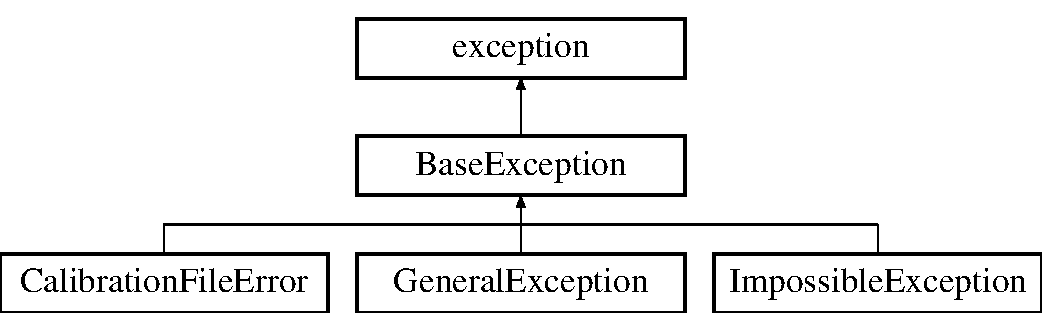
\includegraphics[height=3.000000cm]{class_base_exception}
\end{center}
\end{figure}
\subsection*{Public Member Functions}
\begin{DoxyCompactItemize}
\item 
\hypertarget{class_base_exception_a9a4668c1da76b424a113d600f313b67f}{virtual const char $\ast$ {\bfseries what} () const noexcept=0}\label{class_base_exception_a9a4668c1da76b424a113d600f313b67f}

\end{DoxyCompactItemize}


\subsection{Detailed Description}


Definition at line 10 of file base\-\_\-exception.\-h.



The documentation for this class was generated from the following files\-:\begin{DoxyCompactItemize}
\item 
/home/travis/build/tomas789/tonav/include/exceptions/base\-\_\-exception.\-h\item 
/home/travis/build/tomas789/tonav/src/exceptions/base\-\_\-exception.\-cpp\end{DoxyCompactItemize}

\hypertarget{class_body_state}{\section{Body\-State Class Reference}
\label{class_body_state}\index{Body\-State@{Body\-State}}
}
\subsection*{Public Types}
\begin{DoxyCompactItemize}
\item 
\hypertarget{class_body_state_ac95355c4974335a6f69da770d2de30e0}{using {\bfseries Body\-State\-Type} = Eigen\-::\-Matrix$<$ double, 16, 1 $>$}\label{class_body_state_ac95355c4974335a6f69da770d2de30e0}

\end{DoxyCompactItemize}
\subsection*{Public Member Functions}
\begin{DoxyCompactItemize}
\item 
\hypertarget{class_body_state_a980cbcae469aa1fc0d7efec5248db0d1}{Eigen\-::\-Block$<$ Body\-State\-Type, 4, 1 $>$ {\bfseries get\-Rotation\-Block} ()}\label{class_body_state_a980cbcae469aa1fc0d7efec5248db0d1}

\item 
\hypertarget{class_body_state_a63c1a3704285d7e76a7d7f5a2e4cbafa}{Eigen\-::\-Quaterniond {\bfseries get\-Rotation\-Quaternion} ()}\label{class_body_state_a63c1a3704285d7e76a7d7f5a2e4cbafa}

\item 
\hypertarget{class_body_state_ac1931ea582df06676f52ed72ec26140a}{void {\bfseries set\-Rotation\-Quaternion} (const Eigen\-::\-Quaterniond \&quat)}\label{class_body_state_ac1931ea582df06676f52ed72ec26140a}

\item 
\hypertarget{class_body_state_a1b44594cf450da4c6aa2af1b74fa254a}{Eigen\-::\-Block$<$ Body\-State\-Type, 3, 1 $>$ {\bfseries get\-Position\-Block} ()}\label{class_body_state_a1b44594cf450da4c6aa2af1b74fa254a}

\item 
\hypertarget{class_body_state_a732c36a0723224c49a0b2629081bd26d}{Eigen\-::\-Block$<$ Body\-State\-Type, 3, 1 $>$ {\bfseries get\-Velocity\-Block} ()}\label{class_body_state_a732c36a0723224c49a0b2629081bd26d}

\item 
\hypertarget{class_body_state_adfdecc372089f557d447d9d8e910591f}{Eigen\-::\-Block$<$ Body\-State\-Type, 3, 1 $>$ {\bfseries get\-Accelerometer\-Bias\-Block} ()}\label{class_body_state_adfdecc372089f557d447d9d8e910591f}

\item 
\hypertarget{class_body_state_afd17dde9368642923d7d2c0e49b3afd2}{Eigen\-::\-Block$<$ Body\-State\-Type, 3, 1 $>$ {\bfseries get\-Gyroscope\-Bias\-Block} ()}\label{class_body_state_afd17dde9368642923d7d2c0e49b3afd2}

\end{DoxyCompactItemize}


\subsection{Detailed Description}


Definition at line 7 of file body\-\_\-state.\-h.



The documentation for this class was generated from the following files\-:\begin{DoxyCompactItemize}
\item 
/home/travis/build/tomas789/tonav/include/body\-\_\-state.\-h\item 
/home/travis/build/tomas789/tonav/src/body\-\_\-state.\-cpp\end{DoxyCompactItemize}

\hypertarget{classmsckf_1_1_body_state}{\section{msckf.\-Body\-State Class Reference}
\label{classmsckf_1_1_body_state}\index{msckf.\-Body\-State@{msckf.\-Body\-State}}
}
\subsection*{Public Member Functions}
\begin{DoxyCompactItemize}
\item 
\hypertarget{classmsckf_1_1_body_state_a869468e1c496f460ccef10fe473af84c}{def {\bfseries \-\_\-\-\_\-init\-\_\-\-\_\-}}\label{classmsckf_1_1_body_state_a869468e1c496f460ccef10fe473af84c}

\item 
\hypertarget{classmsckf_1_1_body_state_a7e6fbd3db5a74297588a40ebb9c70fa0}{def {\bfseries time\-\_\-to}}\label{classmsckf_1_1_body_state_a7e6fbd3db5a74297588a40ebb9c70fa0}

\end{DoxyCompactItemize}
\subsection*{Static Public Member Functions}
\begin{DoxyCompactItemize}
\item 
\hypertarget{classmsckf_1_1_body_state_a7b9cebebc5b911a398fe008a17f3f457}{def {\bfseries initialize}}\label{classmsckf_1_1_body_state_a7b9cebebc5b911a398fe008a17f3f457}

\item 
\hypertarget{classmsckf_1_1_body_state_ae376c49e3f60498704092e5295a4355f}{def {\bfseries copy}}\label{classmsckf_1_1_body_state_ae376c49e3f60498704092e5295a4355f}

\item 
\hypertarget{classmsckf_1_1_body_state_a6edd2c5e28633b9ebf2656a2cd9059d2}{def {\bfseries propagate}}\label{classmsckf_1_1_body_state_a6edd2c5e28633b9ebf2656a2cd9059d2}

\end{DoxyCompactItemize}
\subsection*{Public Attributes}
\begin{DoxyCompactItemize}
\item 
\hypertarget{classmsckf_1_1_body_state_ae66c70ddae91a648f29efc568f4344da}{{\bfseries q\-\_\-\-B\-\_\-\-G}}\label{classmsckf_1_1_body_state_ae66c70ddae91a648f29efc568f4344da}

\item 
\hypertarget{classmsckf_1_1_body_state_a0f413de95b39715210b1d88e3d6e707b}{{\bfseries p\-\_\-\-B\-\_\-\-G}}\label{classmsckf_1_1_body_state_a0f413de95b39715210b1d88e3d6e707b}

\item 
\hypertarget{classmsckf_1_1_body_state_aaea8bab90d430f203ff8d8fabd9a16d7}{{\bfseries v\-\_\-\-B\-\_\-\-G}}\label{classmsckf_1_1_body_state_aaea8bab90d430f203ff8d8fabd9a16d7}

\item 
\hypertarget{classmsckf_1_1_body_state_a663d35092ee45633a18a9eab916c7c2a}{{\bfseries time}}\label{classmsckf_1_1_body_state_a663d35092ee45633a18a9eab916c7c2a}

\item 
\hypertarget{classmsckf_1_1_body_state_ac4940afd5c65881731a6a03e090c5093}{{\bfseries rotation\-\_\-estimate}}\label{classmsckf_1_1_body_state_ac4940afd5c65881731a6a03e090c5093}

\item 
\hypertarget{classmsckf_1_1_body_state_a658e340e374f712b049f3197530d3365}{{\bfseries acceleration\-\_\-estimate}}\label{classmsckf_1_1_body_state_a658e340e374f712b049f3197530d3365}

\end{DoxyCompactItemize}
\subsection*{Static Public Attributes}
\begin{DoxyCompactItemize}
\item 
\hypertarget{classmsckf_1_1_body_state_a6ce3e615316fa82782296558cd96e3fb}{tuple {\bfseries global\-\_\-gravity} = np.\-asarray(\mbox{[}0.\-0, 0.\-0, 0\mbox{]})}\label{classmsckf_1_1_body_state_a6ce3e615316fa82782296558cd96e3fb}

\end{DoxyCompactItemize}


\subsection{Detailed Description}


Definition at line 238 of file msckf.\-py.



The documentation for this class was generated from the following file\-:\begin{DoxyCompactItemize}
\item 
/home/travis/build/tomas789/tonav/prototype/msckf.\-py\end{DoxyCompactItemize}

\hypertarget{class_calibration}{\section{Calibration Class Reference}
\label{class_calibration}\index{Calibration@{Calibration}}
}
\subsection*{Public Member Functions}
\begin{DoxyCompactItemize}
\item 
\hypertarget{class_calibration_a0273a577bae64d0833262103580e4a38}{int {\bfseries get\-Max\-Camera\-Poses} () const }\label{class_calibration_a0273a577bae64d0833262103580e4a38}

\item 
\hypertarget{class_calibration_acdf5d45d605b29f9114ae05600f07b76}{int {\bfseries get\-Buffer\-Size} () const }\label{class_calibration_acdf5d45d605b29f9114ae05600f07b76}

\item 
\hypertarget{class_calibration_a681582420d47807e4d8b1c8608e35aef}{int {\bfseries get\-Max\-Triangulation\-Iterations} () const }\label{class_calibration_a681582420d47807e4d8b1c8608e35aef}

\item 
\hypertarget{class_calibration_a871a481190b4ac5a4bb3ae1d5426726e}{Eigen\-::\-Matrix3d {\bfseries get\-Rotation\-From\-Body\-To\-Camera\-Frame} () const }\label{class_calibration_a871a481190b4ac5a4bb3ae1d5426726e}

\item 
\hypertarget{class_calibration_ad3edc4101a92835c6eed1dcfa004b592}{Eigen\-::\-Matrix$<$ double, 3, 3 $>$ {\bfseries get\-G\-Sensitivity\-Matrix} () const }\label{class_calibration_ad3edc4101a92835c6eed1dcfa004b592}

\item 
\hypertarget{class_calibration_a645b1a1cd460d493756669392ac71b78}{Eigen\-::\-Matrix$<$ double, 3, 3 $>$ {\bfseries get\-Gyroscope\-Shape\-Matrix} () const }\label{class_calibration_a645b1a1cd460d493756669392ac71b78}

\item 
\hypertarget{class_calibration_acd1d1fff6512b6fbfa8ff80cd45033f3}{Eigen\-::\-Matrix$<$ double, 3, 3 $>$ {\bfseries get\-Accelerometer\-Shape\-Matrix} () const }\label{class_calibration_acd1d1fff6512b6fbfa8ff80cd45033f3}

\item 
\hypertarget{class_calibration_a1144bc436545a52c5036ba6b02028c78}{Eigen\-::\-Matrix$<$ double, 3, 1 $>$ {\bfseries get\-Camera\-To\-Body\-Offset} () const }\label{class_calibration_a1144bc436545a52c5036ba6b02028c78}

\item 
\hypertarget{class_calibration_ab8e718f8167cbc0d15cb90983175ce9d}{double {\bfseries get\-Focal\-Length\-X} () const }\label{class_calibration_ab8e718f8167cbc0d15cb90983175ce9d}

\item 
\hypertarget{class_calibration_af25283fd143f9f8e4026afadff66188f}{double {\bfseries get\-Focal\-Length\-Y} () const }\label{class_calibration_af25283fd143f9f8e4026afadff66188f}

\item 
\hypertarget{class_calibration_aa101a7999e6eec103dce4ec651c2218b}{double {\bfseries get\-Optical\-Center\-X} () const }\label{class_calibration_aa101a7999e6eec103dce4ec651c2218b}

\item 
\hypertarget{class_calibration_a7486353559a45d424afb1aa6fbfa9f24}{double {\bfseries get\-Optical\-Center\-Y} () const }\label{class_calibration_a7486353559a45d424afb1aa6fbfa9f24}

\item 
\hypertarget{class_calibration_a57798a33c441afe2e0b675008e962af6}{Eigen\-::\-Matrix$<$ double, 3, 1 $>$ {\bfseries get\-Radial\-Distortion\-Parameters} () const }\label{class_calibration_a57798a33c441afe2e0b675008e962af6}

\item 
\hypertarget{class_calibration_ab42ba1d8120e3c22b85204c5dfd98f7f}{Eigen\-::\-Matrix$<$ double, 2, 1 $>$ {\bfseries get\-Tangential\-Distortion\-Parameters} () const }\label{class_calibration_ab42ba1d8120e3c22b85204c5dfd98f7f}

\item 
\hypertarget{class_calibration_a22c6544bba616210e34f9020479a32c6}{double {\bfseries get\-Camera\-Delay\-Time} () const }\label{class_calibration_a22c6544bba616210e34f9020479a32c6}

\item 
\hypertarget{class_calibration_aecbab0b6d724fa68f5af6e038111284b}{double {\bfseries get\-Camera\-Readout\-Time} () const }\label{class_calibration_aecbab0b6d724fa68f5af6e038111284b}

\end{DoxyCompactItemize}
\subsection*{Static Public Member Functions}
\begin{DoxyCompactItemize}
\item 
\hypertarget{class_calibration_a407d16502f36acfc7bd00572abe90739}{static \hyperlink{class_calibration}{Calibration} {\bfseries from\-Path} (boost\-::filesystem\-::path fname)}\label{class_calibration_a407d16502f36acfc7bd00572abe90739}

\item 
\hypertarget{class_calibration_a1d1c3b1b92ae75db9428f61b7afcc7f0}{static bool {\bfseries try\-Parse\-Int} (const std\-::string \&value, int \&out)}\label{class_calibration_a1d1c3b1b92ae75db9428f61b7afcc7f0}

\item 
\hypertarget{class_calibration_a043fc49ab017f6188dfb1b38cf7b573e}{static bool {\bfseries try\-Parse\-Double} (const std\-::string \&value, double \&out)}\label{class_calibration_a043fc49ab017f6188dfb1b38cf7b573e}

\item 
\hypertarget{class_calibration_a58c12342c94ea075107e6202e67c714a}{static bool {\bfseries try\-Parse\-Matrix3d} (const std\-::string \&value, Eigen\-::\-Matrix3d \&out)}\label{class_calibration_a58c12342c94ea075107e6202e67c714a}

\end{DoxyCompactItemize}


\subsection{Detailed Description}


Definition at line 13 of file calibration.\-h.



The documentation for this class was generated from the following files\-:\begin{DoxyCompactItemize}
\item 
/home/travis/build/tomas789/tonav/include/calibration.\-h\item 
/home/travis/build/tomas789/tonav/src/calibration.\-cpp\end{DoxyCompactItemize}

\hypertarget{class_calibration_file_error}{\section{Calibration\-File\-Error Class Reference}
\label{class_calibration_file_error}\index{Calibration\-File\-Error@{Calibration\-File\-Error}}
}
Inheritance diagram for Calibration\-File\-Error\-:\begin{figure}[H]
\begin{center}
\leavevmode
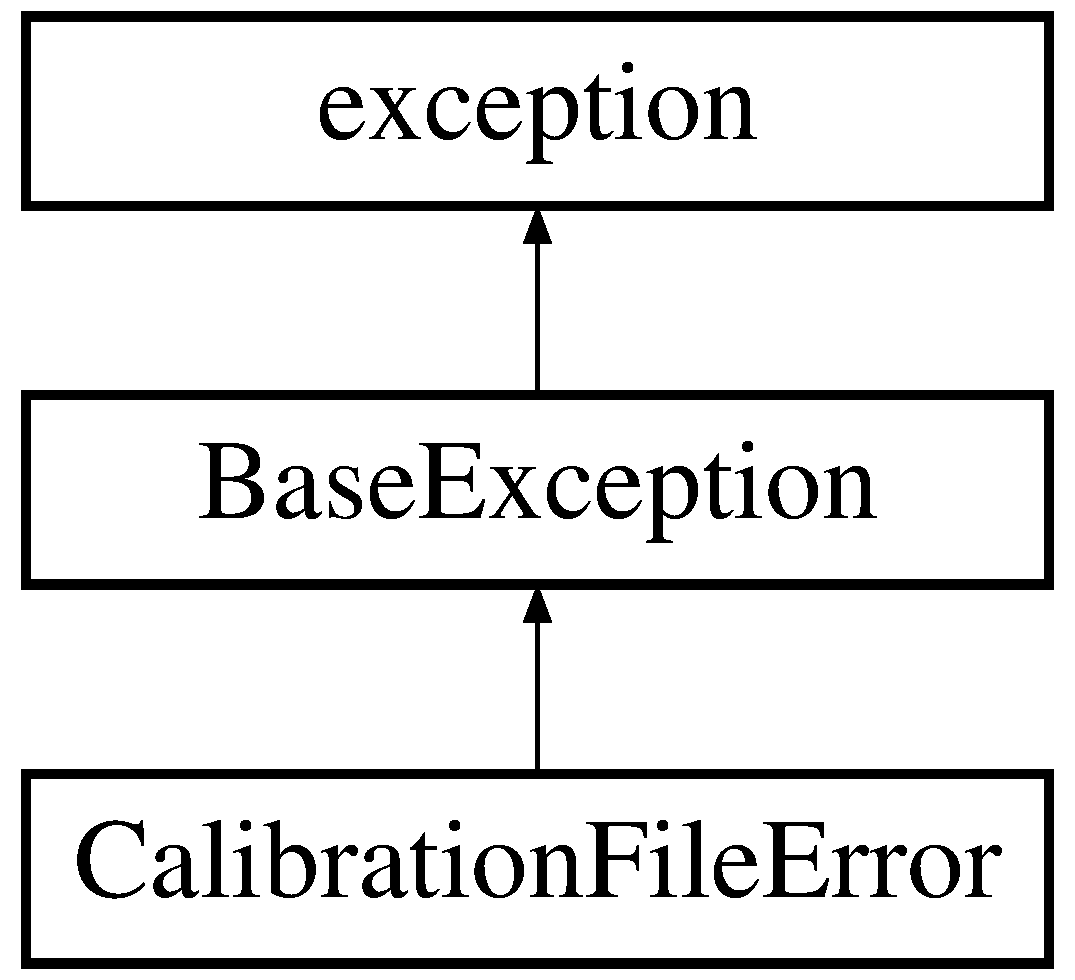
\includegraphics[height=3.000000cm]{class_calibration_file_error}
\end{center}
\end{figure}
\subsection*{Public Member Functions}
\begin{DoxyCompactItemize}
\item 
\hypertarget{class_calibration_file_error_ac4403a65bb13617f6f9aaea23a408c0a}{{\bfseries Calibration\-File\-Error} (const std\-::string \&msg)}\label{class_calibration_file_error_ac4403a65bb13617f6f9aaea23a408c0a}

\item 
\hypertarget{class_calibration_file_error_a91d41fb29208c4304760a251de8ca50a}{{\bfseries Calibration\-File\-Error} (int line\-\_\-number, const std\-::string \&msg)}\label{class_calibration_file_error_a91d41fb29208c4304760a251de8ca50a}

\item 
\hypertarget{class_calibration_file_error_a935a4e242a42bb1ab4867c05f44eebc9}{virtual const char $\ast$ {\bfseries what} () const noexcept}\label{class_calibration_file_error_a935a4e242a42bb1ab4867c05f44eebc9}

\end{DoxyCompactItemize}


\subsection{Detailed Description}


Definition at line 12 of file calibration\-\_\-file\-\_\-error.\-h.



The documentation for this class was generated from the following files\-:\begin{DoxyCompactItemize}
\item 
/home/tomaskrejci/catkin\-\_\-ws/src/tonav/include/exceptions/calibration\-\_\-file\-\_\-error.\-h\item 
/home/tomaskrejci/catkin\-\_\-ws/src/tonav/src/exceptions/calibration\-\_\-file\-\_\-error.\-cpp\end{DoxyCompactItemize}

\hypertarget{class_camera_feed}{\section{Camera\-Feed Class Reference}
\label{class_camera_feed}\index{Camera\-Feed@{Camera\-Feed}}
}
\subsection*{Public Member Functions}
\begin{DoxyCompactItemize}
\item 
\hypertarget{class_camera_feed_a2d7c8c329802b64568b312675115efce}{bool {\bfseries has\-Next} () const }\label{class_camera_feed_a2d7c8c329802b64568b312675115efce}

\item 
\hypertarget{class_camera_feed_a175a707efb56c2f3c78c2859129cbc24}{void {\bfseries next} ()}\label{class_camera_feed_a175a707efb56c2f3c78c2859129cbc24}

\item 
\hypertarget{class_camera_feed_ac703c1de71a7bf488f82921177ea4b0a}{const \hyperlink{class_camera_item}{Camera\-Item} \& {\bfseries top} () const }\label{class_camera_feed_ac703c1de71a7bf488f82921177ea4b0a}

\item 
\hypertarget{class_camera_feed_af761420a0337f52253b23c7d276516f8}{cv\-::\-Mat {\bfseries get\-Image} (const \hyperlink{class_camera_item}{Camera\-Item} \&item) const }\label{class_camera_feed_af761420a0337f52253b23c7d276516f8}

\end{DoxyCompactItemize}
\subsection*{Static Public Member Functions}
\begin{DoxyCompactItemize}
\item 
\hypertarget{class_camera_feed_a38c0ad4632b39babdc99fc65ddc56c36}{static \hyperlink{class_camera_feed}{Camera\-Feed} {\bfseries from\-Dataset} (boost\-::filesystem\-::path path)}\label{class_camera_feed_a38c0ad4632b39babdc99fc65ddc56c36}

\end{DoxyCompactItemize}


\subsection{Detailed Description}


Definition at line 18 of file camera\-\_\-feed.\-h.



The documentation for this class was generated from the following files\-:\begin{DoxyCompactItemize}
\item 
/home/travis/build/tomas789/tonav/include/camera\-\_\-feed.\-h\item 
/home/travis/build/tomas789/tonav/src/camera\-\_\-feed.\-cpp\end{DoxyCompactItemize}

\hypertarget{classmsckf_1_1_camera_item}{\section{msckf.\-Camera\-Item Class Reference}
\label{classmsckf_1_1_camera_item}\index{msckf.\-Camera\-Item@{msckf.\-Camera\-Item}}
}
\subsection*{Public Member Functions}
\begin{DoxyCompactItemize}
\item 
\hypertarget{classmsckf_1_1_camera_item_ab25d363d08d1af7d925814b54d2a5933}{def {\bfseries \-\_\-\-\_\-init\-\_\-\-\_\-}}\label{classmsckf_1_1_camera_item_ab25d363d08d1af7d925814b54d2a5933}

\end{DoxyCompactItemize}
\subsection*{Public Attributes}
\begin{DoxyCompactItemize}
\item 
\hypertarget{classmsckf_1_1_camera_item_ad559a375ad268d16a93220455ecbe38a}{{\bfseries time}}\label{classmsckf_1_1_camera_item_ad559a375ad268d16a93220455ecbe38a}

\item 
\hypertarget{classmsckf_1_1_camera_item_a8d1e979360ecbde8620b03be8760dba8}{{\bfseries image}}\label{classmsckf_1_1_camera_item_a8d1e979360ecbde8620b03be8760dba8}

\end{DoxyCompactItemize}


\subsection{Detailed Description}


Definition at line 149 of file msckf.\-py.



The documentation for this class was generated from the following file\-:\begin{DoxyCompactItemize}
\item 
/home/travis/build/tomas789/tonav/prototype/msckf.\-py\end{DoxyCompactItemize}

\hypertarget{class_camera_item}{\section{Camera\-Item Class Reference}
\label{class_camera_item}\index{Camera\-Item@{Camera\-Item}}
}
\subsection*{Public Member Functions}
\begin{DoxyCompactItemize}
\item 
\hypertarget{class_camera_item_a6227ac10298e97b4ae86371de99cd4c9}{double {\bfseries get\-Time} () const }\label{class_camera_item_a6227ac10298e97b4ae86371de99cd4c9}

\item 
\hypertarget{class_camera_item_a6e19e5bdbfc691fb8abc4e94ef43f05e}{std\-::string {\bfseries get\-File\-Name} () const }\label{class_camera_item_a6e19e5bdbfc691fb8abc4e94ef43f05e}

\end{DoxyCompactItemize}
\subsection*{Static Public Member Functions}
\begin{DoxyCompactItemize}
\item 
\hypertarget{class_camera_item_a4cccf1e169a05288c47ecf232afb2086}{static \hyperlink{class_camera_item}{Camera\-Item} {\bfseries from\-String} (std\-::string fname)}\label{class_camera_item_a4cccf1e169a05288c47ecf232afb2086}

\end{DoxyCompactItemize}


\subsection{Detailed Description}


Definition at line 10 of file camera\-\_\-item.\-h.



The documentation for this class was generated from the following files\-:\begin{DoxyCompactItemize}
\item 
/home/travis/build/tomas789/tonav/include/camera\-\_\-item.\-h\item 
/home/travis/build/tomas789/tonav/src/camera\-\_\-item.\-cpp\end{DoxyCompactItemize}

\hypertarget{class_camera_pose}{\section{Camera\-Pose Class Reference}
\label{class_camera_pose}\index{Camera\-Pose@{Camera\-Pose}}
}
\subsection*{Public Types}
\begin{DoxyCompactItemize}
\item 
\hypertarget{class_camera_pose_a6898788bbfddfab4a5bf78d911477bf4}{using {\bfseries Camera\-Pose\-Type} = Eigen\-::\-Matrix$<$ double, 10, 1 $>$}\label{class_camera_pose_a6898788bbfddfab4a5bf78d911477bf4}

\end{DoxyCompactItemize}
\subsection*{Public Member Functions}
\begin{DoxyCompactItemize}
\item 
\hypertarget{class_camera_pose_a9393e875cfde4b1587a5f8b06d498466}{{\bfseries Camera\-Pose} (std\-::size\-\_\-t pose\-\_\-id)}\label{class_camera_pose_a9393e875cfde4b1587a5f8b06d498466}

\item 
\hypertarget{class_camera_pose_a91fe393ed7bd9c638198a7e138e3926c}{std\-::size\-\_\-t {\bfseries pose\-Id} () const }\label{class_camera_pose_a91fe393ed7bd9c638198a7e138e3926c}

\item 
\hypertarget{class_camera_pose_ab690a1975e061c75e2431c2f671d5637}{std\-::size\-\_\-t {\bfseries get\-Active\-Features\-Count} () const }\label{class_camera_pose_ab690a1975e061c75e2431c2f671d5637}

\item 
\hypertarget{class_camera_pose_ad52f534b1a0b4841a4c8d5e04471f0a1}{void {\bfseries set\-Active\-Features\-Count} (std\-::size\-\_\-t i)}\label{class_camera_pose_ad52f534b1a0b4841a4c8d5e04471f0a1}

\item 
\hypertarget{class_camera_pose_acfe976d10448deee4b714506c3ab6357}{void {\bfseries decrease\-Active\-Features\-Count} ()}\label{class_camera_pose_acfe976d10448deee4b714506c3ab6357}

\item 
\hypertarget{class_camera_pose_adeec70b16372d5aede066da2b6bf5d4a}{Eigen\-::\-Block$<$ Camera\-Pose\-Type, 4, 1 $>$ {\bfseries get\-Rotation\-For\-Body\-Pose\-Block} ()}\label{class_camera_pose_adeec70b16372d5aede066da2b6bf5d4a}

\item 
\hypertarget{class_camera_pose_af518728cc70c31460a20fc0f6f3f40a4}{Eigen\-::\-Block$<$ Camera\-Pose\-Type, 3, 1 $>$ {\bfseries get\-Position\-For\-Body\-Pose\-Block} ()}\label{class_camera_pose_af518728cc70c31460a20fc0f6f3f40a4}

\item 
\hypertarget{class_camera_pose_ae15933c2b5176d011135164962639a99}{Eigen\-::\-Block$<$ Camera\-Pose\-Type, 3, 1 $>$ {\bfseries get\-Velocity\-For\-Body\-Pose\-Block} ()}\label{class_camera_pose_ae15933c2b5176d011135164962639a99}

\item 
\hypertarget{class_camera_pose_aea5ef3206eb4f8929495dfc8f3a93571}{bool {\bfseries is\-Valid} () const }\label{class_camera_pose_aea5ef3206eb4f8929495dfc8f3a93571}

\end{DoxyCompactItemize}


\subsection{Detailed Description}


Definition at line 11 of file camera\-\_\-pose.\-h.



The documentation for this class was generated from the following files\-:\begin{DoxyCompactItemize}
\item 
/home/travis/build/tomas789/tonav/include/camera\-\_\-pose.\-h\item 
/home/travis/build/tomas789/tonav/src/camera\-\_\-pose.\-cpp\end{DoxyCompactItemize}

\hypertarget{class_camera_pose_buffer}{\section{Camera\-Pose\-Buffer Class Reference}
\label{class_camera_pose_buffer}\index{Camera\-Pose\-Buffer@{Camera\-Pose\-Buffer}}
}
\subsection*{Public Types}
\begin{DoxyCompactItemize}
\item 
\hypertarget{class_camera_pose_buffer_a91a3420732c8d8339a8b1dfe7a6e63d3}{using {\bfseries iterator} = boost\-::circular\-\_\-buffer$<$ \hyperlink{class_camera_pose}{Camera\-Pose} $>$\-::iterator}\label{class_camera_pose_buffer_a91a3420732c8d8339a8b1dfe7a6e63d3}

\end{DoxyCompactItemize}
\subsection*{Public Member Functions}
\begin{DoxyCompactItemize}
\item 
\hypertarget{class_camera_pose_buffer_a05b70112084cc230d9c1cac7d886e4d1}{{\bfseries Camera\-Pose\-Buffer} (int max\-\_\-camera\-\_\-poses)}\label{class_camera_pose_buffer_a05b70112084cc230d9c1cac7d886e4d1}

\item 
\hypertarget{class_camera_pose_buffer_a2b49cd0b92c21d0d0c6689c9a1c0fd0f}{void {\bfseries delete\-Oldest\-Camera\-Pose} ()}\label{class_camera_pose_buffer_a2b49cd0b92c21d0d0c6689c9a1c0fd0f}

\item 
\hypertarget{class_camera_pose_buffer_ac159b74f95674855e0161b69249d1e26}{void {\bfseries add\-New\-Camera\-Pose} (const \hyperlink{class_camera_pose}{Camera\-Pose} \&pose)}\label{class_camera_pose_buffer_ac159b74f95674855e0161b69249d1e26}

\item 
\hypertarget{class_camera_pose_buffer_a12612ec4993d931250cfa39d545b0699}{iterator {\bfseries begin} ()}\label{class_camera_pose_buffer_a12612ec4993d931250cfa39d545b0699}

\item 
\hypertarget{class_camera_pose_buffer_a5d8e1318f19521df04bccfe7c01ede23}{iterator {\bfseries end} ()}\label{class_camera_pose_buffer_a5d8e1318f19521df04bccfe7c01ede23}

\item 
\hypertarget{class_camera_pose_buffer_aa7ed926651db6f07f298064862af2791}{\hyperlink{class_camera_pose}{Camera\-Pose} \& {\bfseries front} ()}\label{class_camera_pose_buffer_aa7ed926651db6f07f298064862af2791}

\item 
\hypertarget{class_camera_pose_buffer_a56b8f43d2238bcba3ee9ab0bf232db5e}{\hyperlink{class_camera_pose}{Camera\-Pose} \& {\bfseries back} ()}\label{class_camera_pose_buffer_a56b8f43d2238bcba3ee9ab0bf232db5e}

\item 
\hypertarget{class_camera_pose_buffer_a2692a65ab8a1e38d2e8c607ff46c479d}{std\-::size\-\_\-t {\bfseries size} () const }\label{class_camera_pose_buffer_a2692a65ab8a1e38d2e8c607ff46c479d}

\item 
\hypertarget{class_camera_pose_buffer_a7b9fc93ead67dae155cb1e3cb3c39ddb}{bool {\bfseries empty} () const }\label{class_camera_pose_buffer_a7b9fc93ead67dae155cb1e3cb3c39ddb}

\end{DoxyCompactItemize}


\subsection{Detailed Description}


Definition at line 9 of file camera\-\_\-pose\-\_\-buffer.\-h.



The documentation for this class was generated from the following files\-:\begin{DoxyCompactItemize}
\item 
/home/travis/build/tomas789/tonav/include/camera\-\_\-pose\-\_\-buffer.\-h\item 
/home/travis/build/tomas789/tonav/src/camera\-\_\-pose\-\_\-buffer.\-cpp\end{DoxyCompactItemize}

\hypertarget{classimage__transport_1_1_camera_publisher}{\section{image\-\_\-transport\-:\-:Camera\-Publisher Class Reference}
\label{classimage__transport_1_1_camera_publisher}\index{image\-\_\-transport\-::\-Camera\-Publisher@{image\-\_\-transport\-::\-Camera\-Publisher}}
}


Manages advertisements for publishing camera images.  




{\ttfamily \#include $<$camera\-\_\-publisher.\-h$>$}

\subsection*{Classes}
\begin{DoxyCompactItemize}
\item 
struct \hyperlink{structimage__transport_1_1_camera_publisher_1_1_impl}{Impl}
\end{DoxyCompactItemize}
\subsection*{Public Member Functions}
\begin{DoxyCompactItemize}
\item 
uint32\-\_\-t \hyperlink{classimage__transport_1_1_camera_publisher_a3ab4f35a2549478be6154bb91c6f62e9}{get\-Num\-Subscribers} () const 
\begin{DoxyCompactList}\small\item\em Returns the number of subscribers that are currently connected to this \hyperlink{classimage__transport_1_1_camera_publisher}{Camera\-Publisher}. \end{DoxyCompactList}\item 
\hypertarget{classimage__transport_1_1_camera_publisher_abe9c84e39bb3533e765cd19c9f43607b}{std\-::string \hyperlink{classimage__transport_1_1_camera_publisher_abe9c84e39bb3533e765cd19c9f43607b}{get\-Topic} () const }\label{classimage__transport_1_1_camera_publisher_abe9c84e39bb3533e765cd19c9f43607b}

\begin{DoxyCompactList}\small\item\em Returns the base (image) topic of this \hyperlink{classimage__transport_1_1_camera_publisher}{Camera\-Publisher}. \end{DoxyCompactList}\item 
\hypertarget{classimage__transport_1_1_camera_publisher_a0d99bf10fb26ca65924160d003e71a94}{std\-::string \hyperlink{classimage__transport_1_1_camera_publisher_a0d99bf10fb26ca65924160d003e71a94}{get\-Info\-Topic} () const }\label{classimage__transport_1_1_camera_publisher_a0d99bf10fb26ca65924160d003e71a94}

\begin{DoxyCompactList}\small\item\em Returns the camera info topic of this \hyperlink{classimage__transport_1_1_camera_publisher}{Camera\-Publisher}. \end{DoxyCompactList}\item 
\hypertarget{classimage__transport_1_1_camera_publisher_aaa43f492cde49efe3bfe4192c7ab3c30}{void \hyperlink{classimage__transport_1_1_camera_publisher_aaa43f492cde49efe3bfe4192c7ab3c30}{publish} (const sensor\-\_\-msgs\-::\-Image \&image, const sensor\-\_\-msgs\-::\-Camera\-Info \&info) const }\label{classimage__transport_1_1_camera_publisher_aaa43f492cde49efe3bfe4192c7ab3c30}

\begin{DoxyCompactList}\small\item\em Publish an (image, info) pair on the topics associated with this \hyperlink{classimage__transport_1_1_camera_publisher}{Camera\-Publisher}. \end{DoxyCompactList}\item 
\hypertarget{classimage__transport_1_1_camera_publisher_a9817973953b5c2a4abfcca5e8cdc0417}{void \hyperlink{classimage__transport_1_1_camera_publisher_a9817973953b5c2a4abfcca5e8cdc0417}{publish} (const sensor\-\_\-msgs\-::\-Image\-Const\-Ptr \&image, const sensor\-\_\-msgs\-::\-Camera\-Info\-Const\-Ptr \&info) const }\label{classimage__transport_1_1_camera_publisher_a9817973953b5c2a4abfcca5e8cdc0417}

\begin{DoxyCompactList}\small\item\em Publish an (image, info) pair on the topics associated with this \hyperlink{classimage__transport_1_1_camera_publisher}{Camera\-Publisher}. \end{DoxyCompactList}\item 
void \hyperlink{classimage__transport_1_1_camera_publisher_a711734f50f1f4d1a73e752c98170bd07}{publish} (sensor\-\_\-msgs\-::\-Image \&image, sensor\-\_\-msgs\-::\-Camera\-Info \&info, ros\-::\-Time stamp) const 
\begin{DoxyCompactList}\small\item\em Publish an (image, info) pair with given timestamp on the topics associated with this \hyperlink{classimage__transport_1_1_camera_publisher}{Camera\-Publisher}. \end{DoxyCompactList}\item 
\hypertarget{classimage__transport_1_1_camera_publisher_abf00316990194ba126c371b51f6b2ba8}{void \hyperlink{classimage__transport_1_1_camera_publisher_abf00316990194ba126c371b51f6b2ba8}{shutdown} ()}\label{classimage__transport_1_1_camera_publisher_abf00316990194ba126c371b51f6b2ba8}

\begin{DoxyCompactList}\small\item\em Shutdown the advertisements associated with this \hyperlink{classimage__transport_1_1_publisher}{Publisher}. \end{DoxyCompactList}\item 
\hypertarget{classimage__transport_1_1_camera_publisher_adba3db904b3a92973643130ba0c06134}{{\bfseries operator void $\ast$} () const }\label{classimage__transport_1_1_camera_publisher_adba3db904b3a92973643130ba0c06134}

\item 
\hypertarget{classimage__transport_1_1_camera_publisher_a136a72a44c74bcfa255482c47ece4a0e}{bool {\bfseries operator$<$} (const \hyperlink{classimage__transport_1_1_camera_publisher}{Camera\-Publisher} \&rhs) const }\label{classimage__transport_1_1_camera_publisher_a136a72a44c74bcfa255482c47ece4a0e}

\item 
\hypertarget{classimage__transport_1_1_camera_publisher_a2b156b3a3986144d55389d0c3781c761}{bool {\bfseries operator!=} (const \hyperlink{classimage__transport_1_1_camera_publisher}{Camera\-Publisher} \&rhs) const }\label{classimage__transport_1_1_camera_publisher_a2b156b3a3986144d55389d0c3781c761}

\item 
\hypertarget{classimage__transport_1_1_camera_publisher_ad7c4b4e03ba25e3ab2ae5d15f7ac4d7c}{bool {\bfseries operator==} (const \hyperlink{classimage__transport_1_1_camera_publisher}{Camera\-Publisher} \&rhs) const }\label{classimage__transport_1_1_camera_publisher_ad7c4b4e03ba25e3ab2ae5d15f7ac4d7c}

\end{DoxyCompactItemize}
\subsection*{Friends}
\begin{DoxyCompactItemize}
\item 
\hypertarget{classimage__transport_1_1_camera_publisher_ac010f5a40d98825199e1c5303d0638eb}{class {\bfseries Image\-Transport}}\label{classimage__transport_1_1_camera_publisher_ac010f5a40d98825199e1c5303d0638eb}

\end{DoxyCompactItemize}


\subsection{Detailed Description}
Manages advertisements for publishing camera images. 

\hyperlink{classimage__transport_1_1_camera_publisher}{Camera\-Publisher} is a convenience class for publishing synchronized image and camera info topics using the standard topic naming convention, where the info topic name is \char`\"{}camera\-\_\-info\char`\"{} in the same namespace as the base image topic.

On the client side, \hyperlink{classimage__transport_1_1_camera_subscriber}{Camera\-Subscriber} simplifies subscribing to camera images.

A \hyperlink{classimage__transport_1_1_camera_publisher}{Camera\-Publisher} should always be created through a call to \hyperlink{classimage__transport_1_1_image_transport_ad3b41e47e56b23379043941b2a5ab297}{Image\-Transport\-::advertise\-Camera()}, or copied from one that was. Once all copies of a specific \hyperlink{classimage__transport_1_1_camera_publisher}{Camera\-Publisher} go out of scope, any subscriber callbacks associated with that handle will stop being called. Once all \hyperlink{classimage__transport_1_1_camera_publisher}{Camera\-Publisher} for a given base topic go out of scope the topic (and all subtopics) will be unadvertised. 

Definition at line 62 of file camera\-\_\-publisher.\-h.



\subsection{Member Function Documentation}
\hypertarget{classimage__transport_1_1_camera_publisher_a3ab4f35a2549478be6154bb91c6f62e9}{\index{image\-\_\-transport\-::\-Camera\-Publisher@{image\-\_\-transport\-::\-Camera\-Publisher}!get\-Num\-Subscribers@{get\-Num\-Subscribers}}
\index{get\-Num\-Subscribers@{get\-Num\-Subscribers}!image_transport::CameraPublisher@{image\-\_\-transport\-::\-Camera\-Publisher}}
\subsubsection[{get\-Num\-Subscribers}]{\setlength{\rightskip}{0pt plus 5cm}uint32\-\_\-t image\-\_\-transport\-::\-Camera\-Publisher\-::get\-Num\-Subscribers (
\begin{DoxyParamCaption}
{}
\end{DoxyParamCaption}
) const}}\label{classimage__transport_1_1_camera_publisher_a3ab4f35a2549478be6154bb91c6f62e9}


Returns the number of subscribers that are currently connected to this \hyperlink{classimage__transport_1_1_camera_publisher}{Camera\-Publisher}. 

Returns max(image topic subscribers, info topic subscribers). 

Definition at line 92 of file camera\-\_\-publisher.\-cpp.

\hypertarget{classimage__transport_1_1_camera_publisher_a711734f50f1f4d1a73e752c98170bd07}{\index{image\-\_\-transport\-::\-Camera\-Publisher@{image\-\_\-transport\-::\-Camera\-Publisher}!publish@{publish}}
\index{publish@{publish}!image_transport::CameraPublisher@{image\-\_\-transport\-::\-Camera\-Publisher}}
\subsubsection[{publish}]{\setlength{\rightskip}{0pt plus 5cm}void image\-\_\-transport\-::\-Camera\-Publisher\-::publish (
\begin{DoxyParamCaption}
\item[{sensor\-\_\-msgs\-::\-Image \&}]{image, }
\item[{sensor\-\_\-msgs\-::\-Camera\-Info \&}]{info, }
\item[{ros\-::\-Time}]{stamp}
\end{DoxyParamCaption}
) const}}\label{classimage__transport_1_1_camera_publisher_a711734f50f1f4d1a73e752c98170bd07}


Publish an (image, info) pair with given timestamp on the topics associated with this \hyperlink{classimage__transport_1_1_camera_publisher}{Camera\-Publisher}. 

Convenience version, which sets the timestamps of both image and info to stamp before publishing. 

Definition at line 134 of file camera\-\_\-publisher.\-cpp.



The documentation for this class was generated from the following files\-:\begin{DoxyCompactItemize}
\item 
/home/travis/catkin\-\_\-ws/src/image\-\_\-common/image\-\_\-transport/include/image\-\_\-transport/camera\-\_\-publisher.\-h\item 
/home/travis/catkin\-\_\-ws/src/image\-\_\-common/image\-\_\-transport/src/camera\-\_\-publisher.\-cpp\end{DoxyCompactItemize}

\hypertarget{classimage__transport_1_1_camera_subscriber}{\section{image\-\_\-transport\-:\-:Camera\-Subscriber Class Reference}
\label{classimage__transport_1_1_camera_subscriber}\index{image\-\_\-transport\-::\-Camera\-Subscriber@{image\-\_\-transport\-::\-Camera\-Subscriber}}
}


Manages a subscription callback on synchronized Image and Camera\-Info topics.  




{\ttfamily \#include $<$camera\-\_\-subscriber.\-h$>$}

\subsection*{Classes}
\begin{DoxyCompactItemize}
\item 
struct \hyperlink{structimage__transport_1_1_camera_subscriber_1_1_impl}{Impl}
\end{DoxyCompactItemize}
\subsection*{Public Types}
\begin{DoxyCompactItemize}
\item 
\hypertarget{classimage__transport_1_1_camera_subscriber_abc533a8b0a84b6412549538100aef653}{typedef boost\-::function$<$ void(const \\*
sensor\-\_\-msgs\-::\-Image\-Const\-Ptr \\*
\&, const \\*
sensor\-\_\-msgs\-::\-Camera\-Info\-Const\-Ptr \&)$>$ {\bfseries Callback}}\label{classimage__transport_1_1_camera_subscriber_abc533a8b0a84b6412549538100aef653}

\end{DoxyCompactItemize}
\subsection*{Public Member Functions}
\begin{DoxyCompactItemize}
\item 
\hypertarget{classimage__transport_1_1_camera_subscriber_a52e7e96c56a813de43e9018cdd4640d4}{std\-::string \hyperlink{classimage__transport_1_1_camera_subscriber_a52e7e96c56a813de43e9018cdd4640d4}{get\-Topic} () const }\label{classimage__transport_1_1_camera_subscriber_a52e7e96c56a813de43e9018cdd4640d4}

\begin{DoxyCompactList}\small\item\em Get the base topic (on which the raw image is published). \end{DoxyCompactList}\item 
\hypertarget{classimage__transport_1_1_camera_subscriber_a427737122aa2fa743523aef215f95dfe}{std\-::string \hyperlink{classimage__transport_1_1_camera_subscriber_a427737122aa2fa743523aef215f95dfe}{get\-Info\-Topic} () const }\label{classimage__transport_1_1_camera_subscriber_a427737122aa2fa743523aef215f95dfe}

\begin{DoxyCompactList}\small\item\em Get the camera info topic. \end{DoxyCompactList}\item 
uint32\-\_\-t \hyperlink{classimage__transport_1_1_camera_subscriber_a5dca2655dfe5c885ff992693084530b0}{get\-Num\-Publishers} () const 
\begin{DoxyCompactList}\small\item\em Returns the number of publishers this subscriber is connected to. \end{DoxyCompactList}\item 
\hypertarget{classimage__transport_1_1_camera_subscriber_a31dd4cfcdaaf14d304624d78bcdf4a87}{std\-::string \hyperlink{classimage__transport_1_1_camera_subscriber_a31dd4cfcdaaf14d304624d78bcdf4a87}{get\-Transport} () const }\label{classimage__transport_1_1_camera_subscriber_a31dd4cfcdaaf14d304624d78bcdf4a87}

\begin{DoxyCompactList}\small\item\em Returns the name of the transport being used. \end{DoxyCompactList}\item 
\hypertarget{classimage__transport_1_1_camera_subscriber_aa42ceb9613a14d4c2e297674e52ee684}{void \hyperlink{classimage__transport_1_1_camera_subscriber_aa42ceb9613a14d4c2e297674e52ee684}{shutdown} ()}\label{classimage__transport_1_1_camera_subscriber_aa42ceb9613a14d4c2e297674e52ee684}

\begin{DoxyCompactList}\small\item\em Unsubscribe the callback associated with this \hyperlink{classimage__transport_1_1_camera_subscriber}{Camera\-Subscriber}. \end{DoxyCompactList}\item 
\hypertarget{classimage__transport_1_1_camera_subscriber_af753258daaf280c67bf1c1100bfeb4e4}{{\bfseries operator void $\ast$} () const }\label{classimage__transport_1_1_camera_subscriber_af753258daaf280c67bf1c1100bfeb4e4}

\item 
\hypertarget{classimage__transport_1_1_camera_subscriber_a25fa242f09f9b59190553c73a00ea648}{bool {\bfseries operator$<$} (const \hyperlink{classimage__transport_1_1_camera_subscriber}{Camera\-Subscriber} \&rhs) const }\label{classimage__transport_1_1_camera_subscriber_a25fa242f09f9b59190553c73a00ea648}

\item 
\hypertarget{classimage__transport_1_1_camera_subscriber_ad3d21acca9718dc8ef5367bd4eb136b7}{bool {\bfseries operator!=} (const \hyperlink{classimage__transport_1_1_camera_subscriber}{Camera\-Subscriber} \&rhs) const }\label{classimage__transport_1_1_camera_subscriber_ad3d21acca9718dc8ef5367bd4eb136b7}

\item 
\hypertarget{classimage__transport_1_1_camera_subscriber_af90db2cfc2ca0a99f543c5dbd4f7d216}{bool {\bfseries operator==} (const \hyperlink{classimage__transport_1_1_camera_subscriber}{Camera\-Subscriber} \&rhs) const }\label{classimage__transport_1_1_camera_subscriber_af90db2cfc2ca0a99f543c5dbd4f7d216}

\end{DoxyCompactItemize}
\subsection*{Friends}
\begin{DoxyCompactItemize}
\item 
\hypertarget{classimage__transport_1_1_camera_subscriber_ac010f5a40d98825199e1c5303d0638eb}{class {\bfseries Image\-Transport}}\label{classimage__transport_1_1_camera_subscriber_ac010f5a40d98825199e1c5303d0638eb}

\end{DoxyCompactItemize}


\subsection{Detailed Description}
Manages a subscription callback on synchronized Image and Camera\-Info topics. 

\hyperlink{classimage__transport_1_1_camera_subscriber}{Camera\-Subscriber} is the client-\/side counterpart to \hyperlink{classimage__transport_1_1_camera_publisher}{Camera\-Publisher}, and assumes the same topic naming convention. The callback is of type\-: \begin{DoxyVerb}void callback(const sensor_msgs::ImageConstPtr&, const sensor_msgs::CameraInfoConstPtr&);
\end{DoxyVerb}


A \hyperlink{classimage__transport_1_1_camera_subscriber}{Camera\-Subscriber} should always be created through a call to \hyperlink{classimage__transport_1_1_image_transport_a6754562b0ffe99b0cf716e621d2cfa6b}{Image\-Transport\-::subscribe\-Camera()}, or copied from one that was. Once all copies of a specific \hyperlink{classimage__transport_1_1_camera_subscriber}{Camera\-Subscriber} go out of scope, the subscription callback associated with that handle will stop being called. Once all \hyperlink{classimage__transport_1_1_camera_subscriber}{Camera\-Subscriber} for a given topic go out of scope the topic will be unsubscribed. 

Definition at line 62 of file camera\-\_\-subscriber.\-h.



\subsection{Member Function Documentation}
\hypertarget{classimage__transport_1_1_camera_subscriber_a5dca2655dfe5c885ff992693084530b0}{\index{image\-\_\-transport\-::\-Camera\-Subscriber@{image\-\_\-transport\-::\-Camera\-Subscriber}!get\-Num\-Publishers@{get\-Num\-Publishers}}
\index{get\-Num\-Publishers@{get\-Num\-Publishers}!image_transport::CameraSubscriber@{image\-\_\-transport\-::\-Camera\-Subscriber}}
\subsubsection[{get\-Num\-Publishers}]{\setlength{\rightskip}{0pt plus 5cm}uint32\-\_\-t image\-\_\-transport\-::\-Camera\-Subscriber\-::get\-Num\-Publishers (
\begin{DoxyParamCaption}
{}
\end{DoxyParamCaption}
) const}}\label{classimage__transport_1_1_camera_subscriber_a5dca2655dfe5c885ff992693084530b0}


Returns the number of publishers this subscriber is connected to. 

\begin{DoxyRefDesc}{Todo}
\item[\hyperlink{todo__todo000001}{Todo}]Fix this when message\-\_\-filters\-::\-Subscriber has \hyperlink{classimage__transport_1_1_camera_subscriber_a5dca2655dfe5c885ff992693084530b0}{get\-Num\-Publishers()} \end{DoxyRefDesc}


Definition at line 136 of file camera\-\_\-subscriber.\-cpp.



The documentation for this class was generated from the following files\-:\begin{DoxyCompactItemize}
\item 
/home/travis/catkin\-\_\-ws/src/image\-\_\-common/image\-\_\-transport/include/image\-\_\-transport/camera\-\_\-subscriber.\-h\item 
/home/travis/catkin\-\_\-ws/src/image\-\_\-common/image\-\_\-transport/src/camera\-\_\-subscriber.\-cpp\end{DoxyCompactItemize}

\hypertarget{classpluginlib_1_1_class_loader}{\section{pluginlib\-:\-:Class\-Loader$<$ T $>$ Class Template Reference}
\label{classpluginlib_1_1_class_loader}\index{pluginlib\-::\-Class\-Loader$<$ T $>$@{pluginlib\-::\-Class\-Loader$<$ T $>$}}
}


\subsection{Detailed Description}
\subsubsection*{template$<$class T$>$class pluginlib\-::\-Class\-Loader$<$ T $>$}



Definition at line 42 of file loader\-\_\-fwds.\-h.



The documentation for this class was generated from the following file\-:\begin{DoxyCompactItemize}
\item 
/home/travis/catkin\-\_\-ws/src/image\-\_\-common/image\-\_\-transport/include/image\-\_\-transport/loader\-\_\-fwds.\-h\end{DoxyCompactItemize}

\hypertarget{classestimate__imu__bias_1_1_estimate_imu_bias}{\section{estimate\-\_\-imu\-\_\-bias.\-Estimate\-Imu\-Bias Class Reference}
\label{classestimate__imu__bias_1_1_estimate_imu_bias}\index{estimate\-\_\-imu\-\_\-bias.\-Estimate\-Imu\-Bias@{estimate\-\_\-imu\-\_\-bias.\-Estimate\-Imu\-Bias}}
}
\subsection*{Public Member Functions}
\begin{DoxyCompactItemize}
\item 
\hypertarget{classestimate__imu__bias_1_1_estimate_imu_bias_a40e254ac7e33b9e00766e799c13bfc92}{def {\bfseries \-\_\-\-\_\-init\-\_\-\-\_\-}}\label{classestimate__imu__bias_1_1_estimate_imu_bias_a40e254ac7e33b9e00766e799c13bfc92}

\item 
\hypertarget{classestimate__imu__bias_1_1_estimate_imu_bias_add0fb351b3990a7a5f48398dbd3398d1}{def {\bfseries callback}}\label{classestimate__imu__bias_1_1_estimate_imu_bias_add0fb351b3990a7a5f48398dbd3398d1}

\item 
\hypertarget{classestimate__imu__bias_1_1_estimate_imu_bias_afb5640ffe2885c00f9374d30c282c4ee}{def {\bfseries print\-\_\-results}}\label{classestimate__imu__bias_1_1_estimate_imu_bias_afb5640ffe2885c00f9374d30c282c4ee}

\item 
\hypertarget{classestimate__imu__bias_1_1_estimate_imu_bias_a1a93b692dcc7d2a79ec9dee798fbad65}{def {\bfseries run}}\label{classestimate__imu__bias_1_1_estimate_imu_bias_a1a93b692dcc7d2a79ec9dee798fbad65}

\end{DoxyCompactItemize}
\subsection*{Public Attributes}
\begin{DoxyCompactItemize}
\item 
\hypertarget{classestimate__imu__bias_1_1_estimate_imu_bias_ac85a8cfa7a9b9940e7f6ee5cadda04a0}{{\bfseries data}}\label{classestimate__imu__bias_1_1_estimate_imu_bias_ac85a8cfa7a9b9940e7f6ee5cadda04a0}

\end{DoxyCompactItemize}


\subsection{Detailed Description}


Definition at line 5 of file estimate\-\_\-imu\-\_\-bias.\-py.



The documentation for this class was generated from the following file\-:\begin{DoxyCompactItemize}
\item 
/home/travis/build/tomas789/tonav/tools/estimate\-\_\-imu\-\_\-bias.\-py\end{DoxyCompactItemize}

\hypertarget{classimage__transport_1_1_exception}{\section{image\-\_\-transport\-:\-:Exception Class Reference}
\label{classimage__transport_1_1_exception}\index{image\-\_\-transport\-::\-Exception@{image\-\_\-transport\-::\-Exception}}
}


A base class for all image\-\_\-transport exceptions inheriting from std\-::runtime\-\_\-error.  




{\ttfamily \#include $<$exception.\-h$>$}

Inheritance diagram for image\-\_\-transport\-:\-:Exception\-:\begin{figure}[H]
\begin{center}
\leavevmode
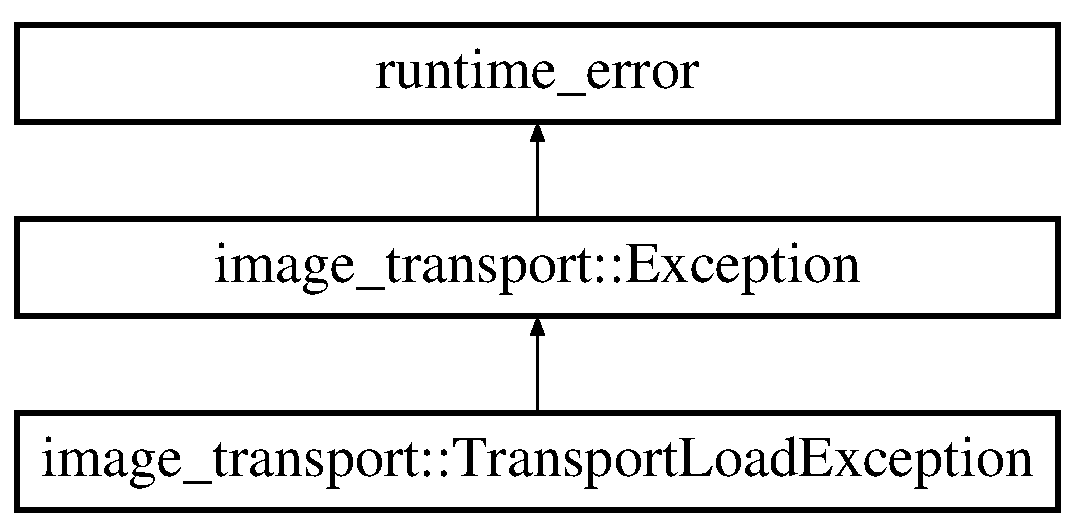
\includegraphics[height=3.000000cm]{classimage__transport_1_1_exception}
\end{center}
\end{figure}
\subsection*{Public Member Functions}
\begin{DoxyCompactItemize}
\item 
\hypertarget{classimage__transport_1_1_exception_a84e9a474ba9e6037e383264d96cec958}{{\bfseries Exception} (const std\-::string \&message)}\label{classimage__transport_1_1_exception_a84e9a474ba9e6037e383264d96cec958}

\end{DoxyCompactItemize}


\subsection{Detailed Description}
A base class for all image\-\_\-transport exceptions inheriting from std\-::runtime\-\_\-error. 

Definition at line 45 of file exception.\-h.



The documentation for this class was generated from the following file\-:\begin{DoxyCompactItemize}
\item 
/home/travis/catkin\-\_\-ws/src/image\-\_\-common/image\-\_\-transport/include/image\-\_\-transport/exception.\-h\end{DoxyCompactItemize}

\hypertarget{class_feature_track}{\section{Feature\-Track Class Reference}
\label{class_feature_track}\index{Feature\-Track@{Feature\-Track}}
}
\subsection*{Public Member Functions}
\begin{DoxyCompactItemize}
\item 
\hypertarget{class_feature_track_ade7f659359480dab8f8ec7ace7625467}{{\bfseries Feature\-Track} (std\-::size\-\_\-t first\-\_\-frame\-\_\-number)}\label{class_feature_track_ade7f659359480dab8f8ec7ace7625467}

\item 
\hypertarget{class_feature_track_a5f13b226ac16fb0c9abe692c17f0f0c6}{void {\bfseries add\-Feature\-Position} (double x, double y)}\label{class_feature_track_a5f13b226ac16fb0c9abe692c17f0f0c6}

\item 
\hypertarget{class_feature_track_aa21cd2b1af1f2aaea1e7d19631f80474}{void {\bfseries revert\-Last\-Position} ()}\label{class_feature_track_aa21cd2b1af1f2aaea1e7d19631f80474}

\item 
\hypertarget{class_feature_track_a1635683732cdfda103a37d926d2efbf9}{std\-::size\-\_\-t {\bfseries get\-First\-Frame\-Number} () const }\label{class_feature_track_a1635683732cdfda103a37d926d2efbf9}

\item 
\hypertarget{class_feature_track_a966f8f018b7305d764216880f4a6f8ba}{bool {\bfseries is\-Out\-Of\-View} () const }\label{class_feature_track_a966f8f018b7305d764216880f4a6f8ba}

\item 
\hypertarget{class_feature_track_a75a507f6ac11d3a9319523d131c7949d}{void {\bfseries set\-Out\-Of\-View} ()}\label{class_feature_track_a75a507f6ac11d3a9319523d131c7949d}

\end{DoxyCompactItemize}


\subsection{Detailed Description}


Definition at line 11 of file feature\-\_\-track.\-h.



The documentation for this class was generated from the following files\-:\begin{DoxyCompactItemize}
\item 
/home/travis/build/tomas789/tonav/include/feature\-\_\-track.\-h\item 
/home/travis/build/tomas789/tonav/src/feature\-\_\-track.\-cpp\end{DoxyCompactItemize}

\hypertarget{classmsckf_1_1_feature_track}{\section{msckf.\-Feature\-Track Class Reference}
\label{classmsckf_1_1_feature_track}\index{msckf.\-Feature\-Track@{msckf.\-Feature\-Track}}
}
\subsection*{Public Member Functions}
\begin{DoxyCompactItemize}
\item 
\hypertarget{classmsckf_1_1_feature_track_aaf665104d4e01547cafe1042c17e9b79}{def {\bfseries \-\_\-\-\_\-init\-\_\-\-\_\-}}\label{classmsckf_1_1_feature_track_aaf665104d4e01547cafe1042c17e9b79}

\item 
\hypertarget{classmsckf_1_1_feature_track_a12f372278b1b14f7553540eb1db21f6f}{def {\bfseries next}}\label{classmsckf_1_1_feature_track_a12f372278b1b14f7553540eb1db21f6f}

\item 
\hypertarget{classmsckf_1_1_feature_track_a08861367ab5e5cce09ef93d2103ef875}{def {\bfseries track\-\_\-length}}\label{classmsckf_1_1_feature_track_a08861367ab5e5cce09ef93d2103ef875}

\item 
\hypertarget{classmsckf_1_1_feature_track_a04d7bc326bd668bb206eaeb36c4355c9}{def {\bfseries get\-\_\-pixel\-\_\-coordinates\-\_\-in\-\_\-image}}\label{classmsckf_1_1_feature_track_a04d7bc326bd668bb206eaeb36c4355c9}

\end{DoxyCompactItemize}
\subsection*{Public Attributes}
\begin{DoxyCompactItemize}
\item 
\hypertarget{classmsckf_1_1_feature_track_a664793a76ba15a7c337eb848aed653b5}{{\bfseries first\-\_\-image}}\label{classmsckf_1_1_feature_track_a664793a76ba15a7c337eb848aed653b5}

\item 
\hypertarget{classmsckf_1_1_feature_track_a91d7ca320a1c0273410fbb4d16ded316}{{\bfseries last\-\_\-image}}\label{classmsckf_1_1_feature_track_a91d7ca320a1c0273410fbb4d16ded316}

\item 
\hypertarget{classmsckf_1_1_feature_track_aa6ac9af251f5d7886075ee3ed2c3d892}{{\bfseries pixel\-\_\-coordinates}}\label{classmsckf_1_1_feature_track_aa6ac9af251f5d7886075ee3ed2c3d892}

\end{DoxyCompactItemize}


\subsection{Detailed Description}


Definition at line 467 of file msckf.\-py.



The documentation for this class was generated from the following file\-:\begin{DoxyCompactItemize}
\item 
/home/travis/build/tomas789/tonav/prototype/msckf.\-py\end{DoxyCompactItemize}

\hypertarget{class_feature_tracker}{\section{Feature\-Tracker Class Reference}
\label{class_feature_tracker}\index{Feature\-Tracker@{Feature\-Tracker}}
}
\subsection*{Public Types}
\begin{DoxyCompactItemize}
\item 
\hypertarget{class_feature_tracker_a8c26ba2ee4c3653c6082a6ceec345f8a}{using {\bfseries feature\-\_\-track\-\_\-list} = std\-::vector$<$ std\-::shared\-\_\-ptr$<$ \hyperlink{class_feature_track}{Feature\-Track} $>$$>$}\label{class_feature_tracker_a8c26ba2ee4c3653c6082a6ceec345f8a}

\end{DoxyCompactItemize}
\subsection*{Public Member Functions}
\begin{DoxyCompactItemize}
\item 
\hypertarget{class_feature_tracker_a1d44cc6cd06ced4f321d2ecebfd7b069}{feature\-\_\-track\-\_\-list {\bfseries process\-Image} (feature\-\_\-track\-\_\-list \&previous\-\_\-tracks, cv\-::\-Mat \&image)}\label{class_feature_tracker_a1d44cc6cd06ced4f321d2ecebfd7b069}

\end{DoxyCompactItemize}


\subsection{Detailed Description}


Definition at line 15 of file feature\-\_\-tracker.\-h.



The documentation for this class was generated from the following files\-:\begin{DoxyCompactItemize}
\item 
/home/tomaskrejci/catkin\-\_\-ws/src/tonav/include/feature\-\_\-tracker.\-h\item 
/home/tomaskrejci/catkin\-\_\-ws/src/tonav/src/feature\-\_\-tracker.\-cpp\end{DoxyCompactItemize}

\hypertarget{class_filter}{\section{Filter Class Reference}
\label{class_filter}\index{Filter@{Filter}}
}


Implementation of M\-S\-C\-K\-F.  




{\ttfamily \#include $<$filter.\-h$>$}

\subsection*{Public Member Functions}
\begin{DoxyCompactItemize}
\item 
\hypertarget{class_filter_ac00d9ce620e60b2c8b26ca9cad7e1b39}{{\bfseries Filter} (const \hyperlink{class_calibration}{Calibration} \&calibration)}\label{class_filter_ac00d9ce620e60b2c8b26ca9cad7e1b39}

\item 
\hypertarget{class_filter_a5742b1247b9f92a9148d99386cdd3876}{void {\bfseries initialize} ()}\label{class_filter_a5742b1247b9f92a9148d99386cdd3876}

\item 
\hypertarget{class_filter_a27176eb65976f98cdc9495b4fdfc3296}{void {\bfseries step\-Inertial} (double timedelta, const \hyperlink{class_imu_item}{Imu\-Item} \&accel, const \hyperlink{class_imu_item}{Imu\-Item} \&gyro)}\label{class_filter_a27176eb65976f98cdc9495b4fdfc3296}

\item 
\hypertarget{class_filter_a1fad49c62892905f713de0bf66d9f3c7}{void {\bfseries step\-Camera} (double timedelta, const \hyperlink{class_imu_item}{Imu\-Item} \&accel, const \hyperlink{class_imu_item}{Imu\-Item} \&gyro, cv\-::\-Mat \&frame)}\label{class_filter_a1fad49c62892905f713de0bf66d9f3c7}

\item 
\hypertarget{class_filter_a3ed7acd6fff45ead8b4209d4e31a8097}{void {\bfseries propagate\-Rotation} (\hyperlink{class_filter_state}{Filter\-State} \&old\-\_\-state, \hyperlink{class_filter_state}{Filter\-State} \&new\-\_\-state, double timedelta, const \hyperlink{class_imu_item}{Imu\-Item} \&accel, const \hyperlink{class_imu_item}{Imu\-Item} \&gyro)}\label{class_filter_a3ed7acd6fff45ead8b4209d4e31a8097}

\item 
\hypertarget{class_filter_a778f444068abe887fd58e02f00be6121}{void {\bfseries propagate\-Velocity\-And\-Position} (\hyperlink{class_filter_state}{Filter\-State} \&old\-\_\-state, \hyperlink{class_filter_state}{Filter\-State} \&new\-\_\-state, double timedelta, const \hyperlink{class_imu_item}{Imu\-Item} \&accel, const \hyperlink{class_imu_item}{Imu\-Item} \&gyro)}\label{class_filter_a778f444068abe887fd58e02f00be6121}

\item 
void \hyperlink{class_filter_ad046b83209a1f03d65ac75f16b538546}{set\-Global\-Gravity} (Eigen\-::\-Vector3d gravity)
\begin{DoxyCompactList}\small\item\em Set initial estimate of gravity in global frame. \end{DoxyCompactList}\item 
\hypertarget{class_filter_aeeb0c2e971a47c73c2f950aa8890f1ac}{Eigen\-::\-Vector3d {\bfseries get\-Global\-Gravity} () const }\label{class_filter_aeeb0c2e971a47c73c2f950aa8890f1ac}

\item 
\hypertarget{class_filter_a936ea0f9f4f587d0cd9bc26a4a73df34}{Eigen\-::\-Vector3d {\bfseries get\-Current\-Position} ()}\label{class_filter_a936ea0f9f4f587d0cd9bc26a4a73df34}

\item 
\hypertarget{class_filter_a7094e57e502a4fc7f124f0d1184eb133}{Eigen\-::\-Quaterniond {\bfseries get\-Current\-Attitude} ()}\label{class_filter_a7094e57e502a4fc7f124f0d1184eb133}

\item 
double \hyperlink{class_filter_a1c7a33a737fafec46d6e98ec1be37a4c}{get\-Image\-Capture\-Time} (double arrive\-\_\-time)
\begin{DoxyCompactList}\small\item\em Calculate $\hat{t} = t + \hat{t}_d$. \end{DoxyCompactList}\end{DoxyCompactItemize}


\subsection{Detailed Description}
Implementation of M\-S\-C\-K\-F. 

This is core functionality of \hyperlink{class_tonav}{Tonav}. All methods must be called with caution. It assumes correct order of update steps.

Don't use this class directly. Use \hyperlink{class_tonav}{Tonav} or \hyperlink{class_tonav_ros}{Tonav\-Ros} instead 

Definition at line 29 of file filter.\-h.



\subsection{Member Function Documentation}
\hypertarget{class_filter_a1c7a33a737fafec46d6e98ec1be37a4c}{\index{Filter@{Filter}!get\-Image\-Capture\-Time@{get\-Image\-Capture\-Time}}
\index{get\-Image\-Capture\-Time@{get\-Image\-Capture\-Time}!Filter@{Filter}}
\subsubsection[{get\-Image\-Capture\-Time}]{\setlength{\rightskip}{0pt plus 5cm}double Filter\-::get\-Image\-Capture\-Time (
\begin{DoxyParamCaption}
\item[{double}]{arrive\-\_\-time}
\end{DoxyParamCaption}
)}}\label{class_filter_a1c7a33a737fafec46d6e98ec1be37a4c}


Calculate $\hat{t} = t + \hat{t}_d$. 

This method calculates image capture time from time when image arrived.


\begin{DoxyParams}{Parameters}
{\em arrive\-\_\-time} & Time whan image arrived \\
\hline
\end{DoxyParams}
\begin{DoxyReturn}{Returns}
Estimated image capture time 
\end{DoxyReturn}


Definition at line 142 of file filter.\-cpp.

\hypertarget{class_filter_ad046b83209a1f03d65ac75f16b538546}{\index{Filter@{Filter}!set\-Global\-Gravity@{set\-Global\-Gravity}}
\index{set\-Global\-Gravity@{set\-Global\-Gravity}!Filter@{Filter}}
\subsubsection[{set\-Global\-Gravity}]{\setlength{\rightskip}{0pt plus 5cm}void Filter\-::set\-Global\-Gravity (
\begin{DoxyParamCaption}
\item[{Eigen\-::\-Vector3d}]{gravity}
\end{DoxyParamCaption}
)}}\label{class_filter_ad046b83209a1f03d65ac75f16b538546}


Set initial estimate of gravity in global frame. 

This is usually calculated as averate of first few accelerometer measurements. It assumes, that device don't move for few seconds at the beginning.


\begin{DoxyParams}{Parameters}
{\em gravity} & Initial estimate of gravity in global frame. \\
\hline
\end{DoxyParams}


Definition at line 126 of file filter.\-cpp.



The documentation for this class was generated from the following files\-:\begin{DoxyCompactItemize}
\item 
/home/travis/build/tomas789/tonav/include/filter.\-h\item 
/home/travis/build/tomas789/tonav/src/filter.\-cpp\end{DoxyCompactItemize}

\hypertarget{class_filter_state}{\section{Filter\-State Class Reference}
\label{class_filter_state}\index{Filter\-State@{Filter\-State}}
}
\subsection*{Public Types}
\begin{DoxyCompactItemize}
\item 
\hypertarget{class_filter_state_a26539bef949b11d11deb68ab8fba5598}{using {\bfseries State\-Type} = Eigen\-::\-Matrix$<$ double, 57, 1 $>$}\label{class_filter_state_a26539bef949b11d11deb68ab8fba5598}

\end{DoxyCompactItemize}
\subsection*{Public Member Functions}
\begin{DoxyCompactItemize}
\item 
\hypertarget{class_filter_state_a549088ec74cb2262e397b929abc174d2}{Eigen\-::\-Block$<$ State\-Type, 4, 1 $>$ {\bfseries get\-Rotation\-Block} ()}\label{class_filter_state_a549088ec74cb2262e397b929abc174d2}

\item 
\hypertarget{class_filter_state_a5f61beb08bf43811cebea645c80949ac}{Eigen\-::\-Quaterniond {\bfseries get\-Rotation\-Quaternion} ()}\label{class_filter_state_a5f61beb08bf43811cebea645c80949ac}

\item 
\hypertarget{class_filter_state_ab2a6e477d01da9521267781a73757838}{void {\bfseries set\-Rotation\-Quaternion} (const Eigen\-::\-Quaterniond \&quat)}\label{class_filter_state_ab2a6e477d01da9521267781a73757838}

\item 
\hypertarget{class_filter_state_af2dd9af9a0722a05cbc59981cf40aead}{Eigen\-::\-Block$<$ State\-Type, 3, 1 $>$ {\bfseries get\-Position\-Block} ()}\label{class_filter_state_af2dd9af9a0722a05cbc59981cf40aead}

\item 
\hypertarget{class_filter_state_a239c2732f1a3d647c21b96f5d53dd215}{Eigen\-::\-Block$<$ State\-Type, 3, 1 $>$ {\bfseries get\-Velocity\-Block} ()}\label{class_filter_state_a239c2732f1a3d647c21b96f5d53dd215}

\item 
\hypertarget{class_filter_state_a43b485d8c02d6eb8e37cd8f2323e9e43}{Eigen\-::\-Block$<$ State\-Type, 3, 1 $>$ {\bfseries get\-Accelerometer\-Bias\-Block} ()}\label{class_filter_state_a43b485d8c02d6eb8e37cd8f2323e9e43}

\item 
\hypertarget{class_filter_state_a8bb562801b8b34026dad74bd4223c06e}{Eigen\-::\-Block$<$ State\-Type, 3, 1 $>$ {\bfseries get\-Gyroscope\-Bias\-Block} ()}\label{class_filter_state_a8bb562801b8b34026dad74bd4223c06e}

\item 
\hypertarget{class_filter_state_a8686bb8e54e2e9902c28095f8c623745}{Eigen\-::\-Block$<$ State\-Type, 9, 1 $>$ {\bfseries get\-Gyroscope\-Shape\-Vectorized\-Block} ()}\label{class_filter_state_a8686bb8e54e2e9902c28095f8c623745}

\item 
\hypertarget{class_filter_state_a1ab46a729807178faf9b6bebb87aa791}{Eigen\-::\-Block$<$ State\-Type, 9, 1 $>$ {\bfseries get\-G\-Sensitivity\-Vectorized\-Block} ()}\label{class_filter_state_a1ab46a729807178faf9b6bebb87aa791}

\item 
\hypertarget{class_filter_state_a57cb64b2b25132c2da38b0313da415c5}{Eigen\-::\-Block$<$ State\-Type, 9, 1 $>$ {\bfseries get\-Accelerometer\-Shape\-Vectorized\-Block} ()}\label{class_filter_state_a57cb64b2b25132c2da38b0313da415c5}

\item 
\hypertarget{class_filter_state_a844855f0fa5ebf0c606a06ea6fdb460b}{Eigen\-::\-Block$<$ State\-Type, 3, 1 $>$ {\bfseries get\-Camera\-To\-Body\-Offset\-Block} ()}\label{class_filter_state_a844855f0fa5ebf0c606a06ea6fdb460b}

\item 
\hypertarget{class_filter_state_a3b65a9649366c853ffd99784fe9bef72}{double \& {\bfseries get\-Focal\-Length\-X\-Ref} ()}\label{class_filter_state_a3b65a9649366c853ffd99784fe9bef72}

\item 
\hypertarget{class_filter_state_aed71d6cec7d8a101ba10b83f969d28d4}{double \& {\bfseries get\-Focal\-Length\-Y\-Ref} ()}\label{class_filter_state_aed71d6cec7d8a101ba10b83f969d28d4}

\item 
\hypertarget{class_filter_state_a3fc41a17c48851340acbfdfc9c164f01}{double \& {\bfseries get\-Optical\-Center\-X\-Ref} ()}\label{class_filter_state_a3fc41a17c48851340acbfdfc9c164f01}

\item 
\hypertarget{class_filter_state_a7ddf9eca9ab6cad9bee85ee6cfc80de0}{double \& {\bfseries get\-Optical\-Center\-Y\-Ref} ()}\label{class_filter_state_a7ddf9eca9ab6cad9bee85ee6cfc80de0}

\item 
\hypertarget{class_filter_state_aa326b846da2b55623e4d219d357e6b57}{Eigen\-::\-Block$<$ State\-Type, 3, 1 $>$ {\bfseries get\-Radial\-Distortion\-Parameters\-Block} ()}\label{class_filter_state_aa326b846da2b55623e4d219d357e6b57}

\item 
\hypertarget{class_filter_state_ad4b9c49509f2cc303c554969a8264c89}{Eigen\-::\-Block$<$ State\-Type, 2, 1 $>$ {\bfseries get\-Tangential\-Distortion\-Parameters\-Block} ()}\label{class_filter_state_ad4b9c49509f2cc303c554969a8264c89}

\item 
\hypertarget{class_filter_state_a6563a73bad1016317018c85d53380962}{double \& {\bfseries get\-Camera\-Delay\-Time\-Ref} ()}\label{class_filter_state_a6563a73bad1016317018c85d53380962}

\item 
\hypertarget{class_filter_state_ab9d3e7cad1ae09ed35bcc528c0e8ef45}{double \& {\bfseries get\-Camera\-Readout\-Time\-Ref} ()}\label{class_filter_state_ab9d3e7cad1ae09ed35bcc528c0e8ef45}

\item 
\hypertarget{class_filter_state_a928bd10a77b39859d6f108f8dd8ae0e9}{Eigen\-::\-Block$<$ Eigen\-::\-Vector3d, 3, 1 $>$ {\bfseries get\-Rotation\-Estimate\-Block} ()}\label{class_filter_state_a928bd10a77b39859d6f108f8dd8ae0e9}

\item 
\hypertarget{class_filter_state_a4436166f7dbaf6c002b6fc2832b4f136}{Eigen\-::\-Block$<$ Eigen\-::\-Vector3d, 3, 1 $>$ {\bfseries get\-Acceleration\-Estimate\-Block} ()}\label{class_filter_state_a4436166f7dbaf6c002b6fc2832b4f136}

\item 
\hypertarget{class_filter_state_ab3d02580cdbd89bc64276467d7c1c854}{Eigen\-::\-Quaterniond {\bfseries get\-Rotation\-To\-This\-Frame} ()}\label{class_filter_state_ab3d02580cdbd89bc64276467d7c1c854}

\item 
\hypertarget{class_filter_state_ae820e97a5a74c7765780bc7bb223796b}{void {\bfseries set\-Rotation\-To\-This\-Frame} (const Eigen\-::\-Quaterniond \&quat)}\label{class_filter_state_ae820e97a5a74c7765780bc7bb223796b}

\item 
\hypertarget{class_filter_state_aed4aab3a5133d37924bc5c1284b6cb66}{std\-::ostream \& {\bfseries ugly\-Print} (std\-::ostream \&out) const }\label{class_filter_state_aed4aab3a5133d37924bc5c1284b6cb66}

\item 
\hypertarget{class_filter_state_af33cfbc67284846e3ca9c26a79c227a9}{\hyperlink{class_filter_state}{Filter\-State} {\bfseries derive\-New\-State\-For\-Imu\-Propagation} () const }\label{class_filter_state_af33cfbc67284846e3ca9c26a79c227a9}

\item 
\hypertarget{class_filter_state_a9fdc71df11cf72369b86be2eaffcea27}{void {\bfseries append\-Camera\-Pose} (const \hyperlink{class_camera_pose}{Camera\-Pose} \&camera\-\_\-pose)}\label{class_filter_state_a9fdc71df11cf72369b86be2eaffcea27}

\end{DoxyCompactItemize}


\subsection{Detailed Description}


Definition at line 14 of file filter\-\_\-state.\-h.



The documentation for this class was generated from the following files\-:\begin{DoxyCompactItemize}
\item 
/home/tomaskrejci/catkin\-\_\-ws/src/tonav/include/filter\-\_\-state.\-h\item 
/home/tomaskrejci/catkin\-\_\-ws/src/tonav/src/filter\-\_\-state.\-cpp\end{DoxyCompactItemize}

\hypertarget{class_frame_features}{\section{Frame\-Features Class Reference}
\label{class_frame_features}\index{Frame\-Features@{Frame\-Features}}
}
\subsection*{Public Member Functions}
\begin{DoxyCompactItemize}
\item 
\hypertarget{class_frame_features_a6977a4effbe856ff8583f4352cd138b8}{std\-::vector$<$ cv\-::\-D\-Match $>$ {\bfseries match} (cv\-::\-Ptr$<$ cv\-::\-Descriptor\-Matcher $>$ matcher, const \hyperlink{class_frame_features}{Frame\-Features} \&other)}\label{class_frame_features_a6977a4effbe856ff8583f4352cd138b8}

\item 
\hypertarget{class_frame_features_ae36e05c015c5980fb0801fc0b6ee97ca}{void {\bfseries draw\-Features} (cv\-::\-Mat \&image, cv\-::\-Scalar color=cv\-::\-Scalar(255, 0, 0))}\label{class_frame_features_ae36e05c015c5980fb0801fc0b6ee97ca}

\item 
\hypertarget{class_frame_features_aff3c47e301fde7db68ecac5d852c6edf}{std\-::vector$<$ cv\-::\-Key\-Point $>$ \& {\bfseries keypoints} ()}\label{class_frame_features_aff3c47e301fde7db68ecac5d852c6edf}

\item 
\hypertarget{class_frame_features_a29b51fc67b07fe6e5b9236a092d1e17a}{const std\-::vector$<$ cv\-::\-Key\-Point $>$ \& {\bfseries keypoints} () const }\label{class_frame_features_a29b51fc67b07fe6e5b9236a092d1e17a}

\end{DoxyCompactItemize}
\subsection*{Static Public Member Functions}
\begin{DoxyCompactItemize}
\item 
\hypertarget{class_frame_features_a5942b53a2e105a82e6454cd259157aa0}{static \hyperlink{class_frame_features}{Frame\-Features} {\bfseries from\-Image} (cv\-::\-Ptr$<$ cv\-::\-Feature\-Detector $>$ detector, cv\-::\-Ptr$<$ cv\-::\-Descriptor\-Extractor $>$ extractor, cv\-::\-Mat \&image)}\label{class_frame_features_a5942b53a2e105a82e6454cd259157aa0}

\end{DoxyCompactItemize}


\subsection{Detailed Description}


Definition at line 11 of file frame\-\_\-features.\-h.



The documentation for this class was generated from the following files\-:\begin{DoxyCompactItemize}
\item 
/home/travis/build/tomas789/tonav/include/frame\-\_\-features.\-h\item 
/home/travis/build/tomas789/tonav/src/frame\-\_\-features.\-cpp\end{DoxyCompactItemize}

\hypertarget{class_general_exception}{\section{General\-Exception Class Reference}
\label{class_general_exception}\index{General\-Exception@{General\-Exception}}
}
Inheritance diagram for General\-Exception\-:\begin{figure}[H]
\begin{center}
\leavevmode
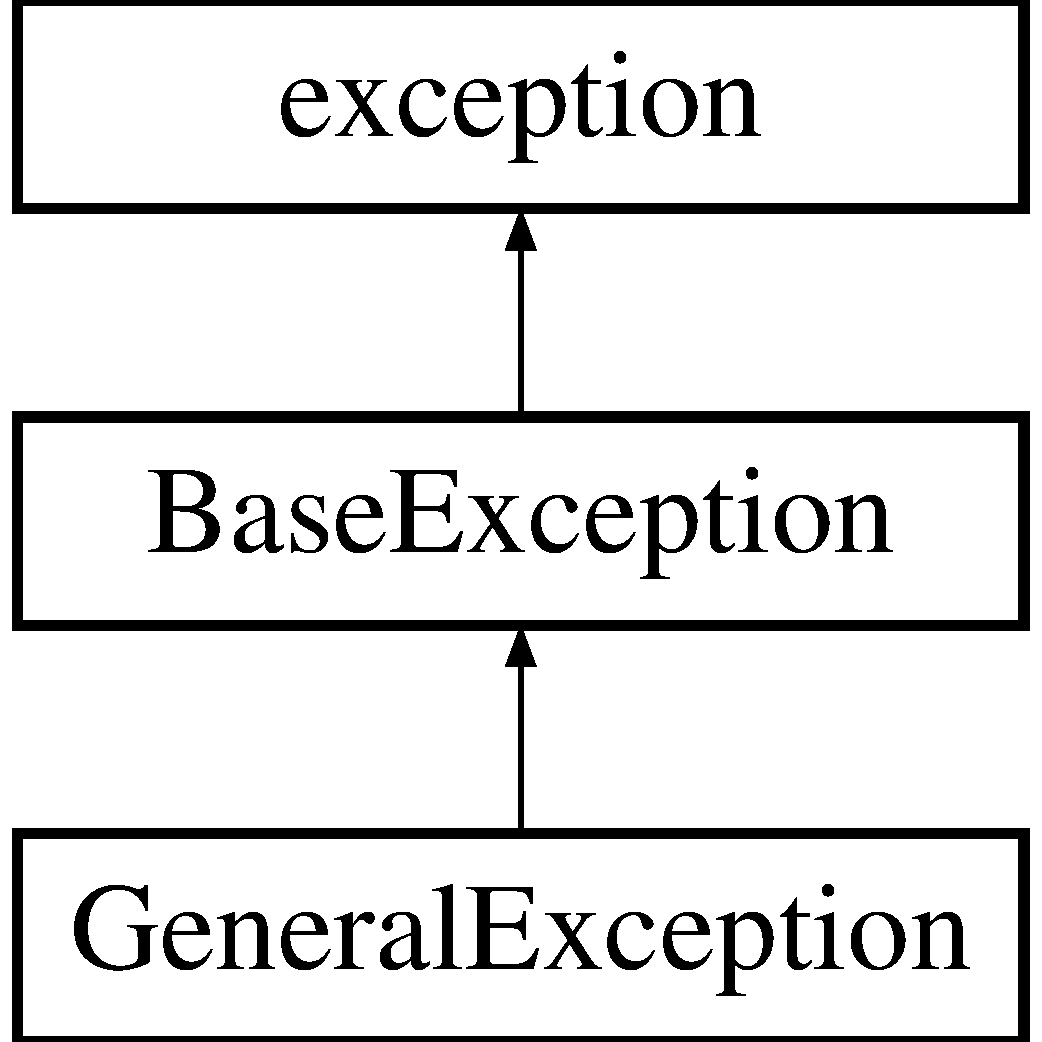
\includegraphics[height=3.000000cm]{class_general_exception}
\end{center}
\end{figure}
\subsection*{Public Member Functions}
\begin{DoxyCompactItemize}
\item 
\hypertarget{class_general_exception_ae9a9599d82aa29bef098dbb594e2f13e}{{\bfseries General\-Exception} (const std\-::string \&msg)}\label{class_general_exception_ae9a9599d82aa29bef098dbb594e2f13e}

\item 
\hypertarget{class_general_exception_ab6bb7c8ae3ab248e082d7fbf3f4a2cf3}{{\bfseries General\-Exception} (int line\-\_\-number, const std\-::string \&msg)}\label{class_general_exception_ab6bb7c8ae3ab248e082d7fbf3f4a2cf3}

\item 
\hypertarget{class_general_exception_a1d8d27063e77fe4658daa8279d0af52c}{virtual const char $\ast$ {\bfseries what} () const noexcept}\label{class_general_exception_a1d8d27063e77fe4658daa8279d0af52c}

\end{DoxyCompactItemize}


\subsection{Detailed Description}


Definition at line 12 of file general\-\_\-exception.\-h.



The documentation for this class was generated from the following files\-:\begin{DoxyCompactItemize}
\item 
/home/tomaskrejci/catkin\-\_\-ws/src/tonav/include/exceptions/general\-\_\-exception.\-h\item 
/home/tomaskrejci/catkin\-\_\-ws/src/tonav/src/exceptions/general\-\_\-exception.\-cpp\end{DoxyCompactItemize}

\hypertarget{classmsckf_1_1_image_tracker}{\section{msckf.\-Image\-Tracker Class Reference}
\label{classmsckf_1_1_image_tracker}\index{msckf.\-Image\-Tracker@{msckf.\-Image\-Tracker}}
}
\subsection*{Public Member Functions}
\begin{DoxyCompactItemize}
\item 
\hypertarget{classmsckf_1_1_image_tracker_a6cda7073370f94e89f1cf3c5181699be}{def {\bfseries \-\_\-\-\_\-init\-\_\-\-\_\-}}\label{classmsckf_1_1_image_tracker_a6cda7073370f94e89f1cf3c5181699be}

\item 
\hypertarget{classmsckf_1_1_image_tracker_ae642350c572cf0e46ec37d07ba7ee975}{def {\bfseries track\-\_\-next}}\label{classmsckf_1_1_image_tracker_ae642350c572cf0e46ec37d07ba7ee975}

\item 
\hypertarget{classmsckf_1_1_image_tracker_ab4bc5433e45f2c83c18951fe2a3f5aa1}{def {\bfseries extract\-\_\-old\-\_\-features}}\label{classmsckf_1_1_image_tracker_ab4bc5433e45f2c83c18951fe2a3f5aa1}

\item 
\hypertarget{classmsckf_1_1_image_tracker_aaae69c20884145a31bb9aca56ad0e475}{def {\bfseries image\-\_\-to\-\_\-publish}}\label{classmsckf_1_1_image_tracker_aaae69c20884145a31bb9aca56ad0e475}

\end{DoxyCompactItemize}
\subsection*{Public Attributes}
\begin{DoxyCompactItemize}
\item 
\hypertarget{classmsckf_1_1_image_tracker_ac0bdc5e455ec9a9e179f88576444678a}{{\bfseries image\-\_\-counter}}\label{classmsckf_1_1_image_tracker_ac0bdc5e455ec9a9e179f88576444678a}

\item 
\hypertarget{classmsckf_1_1_image_tracker_a5f3fcf1a20788c99f16a3ead38a0931e}{{\bfseries last\-\_\-image}}\label{classmsckf_1_1_image_tracker_a5f3fcf1a20788c99f16a3ead38a0931e}

\item 
\hypertarget{classmsckf_1_1_image_tracker_a6b825a2e9b42766b1ab8c0781ecc5a41}{{\bfseries last\-\_\-kps}}\label{classmsckf_1_1_image_tracker_a6b825a2e9b42766b1ab8c0781ecc5a41}

\item 
\hypertarget{classmsckf_1_1_image_tracker_a8cd7b9cfc26ad48bc0adfa8da1e0edcb}{{\bfseries last\-\_\-des}}\label{classmsckf_1_1_image_tracker_a8cd7b9cfc26ad48bc0adfa8da1e0edcb}

\item 
\hypertarget{classmsckf_1_1_image_tracker_a2764caa363b3ff3de9f854b47977947d}{{\bfseries last\-\_\-image\-\_\-was\-\_\-published}}\label{classmsckf_1_1_image_tracker_a2764caa363b3ff3de9f854b47977947d}

\item 
\hypertarget{classmsckf_1_1_image_tracker_a61d25a81ca62500d4b64b3c216817e68}{{\bfseries last\-\_\-matches\-\_\-image}}\label{classmsckf_1_1_image_tracker_a61d25a81ca62500d4b64b3c216817e68}

\item 
\hypertarget{classmsckf_1_1_image_tracker_a5c21c3f90f387f6f1d50814105736ad6}{{\bfseries last\-\_\-features}}\label{classmsckf_1_1_image_tracker_a5c21c3f90f387f6f1d50814105736ad6}

\item 
\hypertarget{classmsckf_1_1_image_tracker_af04b2528381cdaa7ad4ff2558f1634f3}{{\bfseries orb}}\label{classmsckf_1_1_image_tracker_af04b2528381cdaa7ad4ff2558f1634f3}

\item 
\hypertarget{classmsckf_1_1_image_tracker_a3b793e2f18c9c29fe8a584d9974c1b6a}{{\bfseries matcher}}\label{classmsckf_1_1_image_tracker_a3b793e2f18c9c29fe8a584d9974c1b6a}

\end{DoxyCompactItemize}


\subsection{Detailed Description}


Definition at line 486 of file msckf.\-py.



The documentation for this class was generated from the following file\-:\begin{DoxyCompactItemize}
\item 
/home/travis/build/tomas789/tonav/prototype/msckf.\-py\end{DoxyCompactItemize}

\hypertarget{classimage__transport_1_1_image_transport}{\section{image\-\_\-transport\-:\-:Image\-Transport Class Reference}
\label{classimage__transport_1_1_image_transport}\index{image\-\_\-transport\-::\-Image\-Transport@{image\-\_\-transport\-::\-Image\-Transport}}
}


Advertise and subscribe to image topics.  




{\ttfamily \#include $<$image\-\_\-transport.\-h$>$}

\subsection*{Classes}
\begin{DoxyCompactItemize}
\item 
struct \hyperlink{structimage__transport_1_1_image_transport_1_1_impl}{Impl}
\end{DoxyCompactItemize}
\subsection*{Public Member Functions}
\begin{DoxyCompactItemize}
\item 
\hypertarget{classimage__transport_1_1_image_transport_aeffb763301848fa9ead353568bb1c150}{{\bfseries Image\-Transport} (const ros\-::\-Node\-Handle \&nh)}\label{classimage__transport_1_1_image_transport_aeffb763301848fa9ead353568bb1c150}

\item 
\hypertarget{classimage__transport_1_1_image_transport_aba83e00cf60977d58ac17c2915f2562b}{\hyperlink{classimage__transport_1_1_publisher}{Publisher} \hyperlink{classimage__transport_1_1_image_transport_aba83e00cf60977d58ac17c2915f2562b}{advertise} (const std\-::string \&base\-\_\-topic, uint32\-\_\-t queue\-\_\-size, bool latch=false)}\label{classimage__transport_1_1_image_transport_aba83e00cf60977d58ac17c2915f2562b}

\begin{DoxyCompactList}\small\item\em Advertise an image topic, simple version. \end{DoxyCompactList}\item 
\hypertarget{classimage__transport_1_1_image_transport_aa66ce930baa92b21a84956b289340671}{\hyperlink{classimage__transport_1_1_publisher}{Publisher} \hyperlink{classimage__transport_1_1_image_transport_aa66ce930baa92b21a84956b289340671}{advertise} (const std\-::string \&base\-\_\-topic, uint32\-\_\-t queue\-\_\-size, const Subscriber\-Status\-Callback \&connect\-\_\-cb, const Subscriber\-Status\-Callback \&disconnect\-\_\-cb=Subscriber\-Status\-Callback(), const ros\-::\-Void\-Ptr \&tracked\-\_\-object=ros\-::\-Void\-Ptr(), bool latch=false)}\label{classimage__transport_1_1_image_transport_aa66ce930baa92b21a84956b289340671}

\begin{DoxyCompactList}\small\item\em Advertise an image topic with subcriber status callbacks. \end{DoxyCompactList}\item 
\hypertarget{classimage__transport_1_1_image_transport_a1c847a2c719c874f84a78a6a60b98c7f}{\hyperlink{classimage__transport_1_1_subscriber}{Subscriber} \hyperlink{classimage__transport_1_1_image_transport_a1c847a2c719c874f84a78a6a60b98c7f}{subscribe} (const std\-::string \&base\-\_\-topic, uint32\-\_\-t queue\-\_\-size, const boost\-::function$<$ void(const sensor\-\_\-msgs\-::\-Image\-Const\-Ptr \&)$>$ \&callback, const ros\-::\-Void\-Ptr \&tracked\-\_\-object=ros\-::\-Void\-Ptr(), const \hyperlink{classimage__transport_1_1_transport_hints}{Transport\-Hints} \&transport\-\_\-hints=\hyperlink{classimage__transport_1_1_transport_hints}{Transport\-Hints}())}\label{classimage__transport_1_1_image_transport_a1c847a2c719c874f84a78a6a60b98c7f}

\begin{DoxyCompactList}\small\item\em Subscribe to an image topic, version for arbitrary boost\-::function object. \end{DoxyCompactList}\item 
\hypertarget{classimage__transport_1_1_image_transport_a1a2ae66942f19a127739fe062236e7f3}{\hyperlink{classimage__transport_1_1_subscriber}{Subscriber} \hyperlink{classimage__transport_1_1_image_transport_a1a2ae66942f19a127739fe062236e7f3}{subscribe} (const std\-::string \&base\-\_\-topic, uint32\-\_\-t queue\-\_\-size, void($\ast$fp)(const sensor\-\_\-msgs\-::\-Image\-Const\-Ptr \&), const \hyperlink{classimage__transport_1_1_transport_hints}{Transport\-Hints} \&transport\-\_\-hints=\hyperlink{classimage__transport_1_1_transport_hints}{Transport\-Hints}())}\label{classimage__transport_1_1_image_transport_a1a2ae66942f19a127739fe062236e7f3}

\begin{DoxyCompactList}\small\item\em Subscribe to an image topic, version for bare function. \end{DoxyCompactList}\item 
\hypertarget{classimage__transport_1_1_image_transport_a0016526367fba9df0ca326d570e84bb2}{{\footnotesize template$<$class T $>$ }\\\hyperlink{classimage__transport_1_1_subscriber}{Subscriber} \hyperlink{classimage__transport_1_1_image_transport_a0016526367fba9df0ca326d570e84bb2}{subscribe} (const std\-::string \&base\-\_\-topic, uint32\-\_\-t queue\-\_\-size, void(T\-::$\ast$fp)(const sensor\-\_\-msgs\-::\-Image\-Const\-Ptr \&), T $\ast$obj, const \hyperlink{classimage__transport_1_1_transport_hints}{Transport\-Hints} \&transport\-\_\-hints=\hyperlink{classimage__transport_1_1_transport_hints}{Transport\-Hints}())}\label{classimage__transport_1_1_image_transport_a0016526367fba9df0ca326d570e84bb2}

\begin{DoxyCompactList}\small\item\em Subscribe to an image topic, version for class member function with bare pointer. \end{DoxyCompactList}\item 
\hypertarget{classimage__transport_1_1_image_transport_aadba56ce8213440b0de988aadd27e2bf}{{\footnotesize template$<$class T $>$ }\\\hyperlink{classimage__transport_1_1_subscriber}{Subscriber} \hyperlink{classimage__transport_1_1_image_transport_aadba56ce8213440b0de988aadd27e2bf}{subscribe} (const std\-::string \&base\-\_\-topic, uint32\-\_\-t queue\-\_\-size, void(T\-::$\ast$fp)(const sensor\-\_\-msgs\-::\-Image\-Const\-Ptr \&), const boost\-::shared\-\_\-ptr$<$ T $>$ \&obj, const \hyperlink{classimage__transport_1_1_transport_hints}{Transport\-Hints} \&transport\-\_\-hints=\hyperlink{classimage__transport_1_1_transport_hints}{Transport\-Hints}())}\label{classimage__transport_1_1_image_transport_aadba56ce8213440b0de988aadd27e2bf}

\begin{DoxyCompactList}\small\item\em Subscribe to an image topic, version for class member function with shared\-\_\-ptr. \end{DoxyCompactList}\item 
\hypertarget{classimage__transport_1_1_image_transport_ad3b41e47e56b23379043941b2a5ab297}{\hyperlink{classimage__transport_1_1_camera_publisher}{Camera\-Publisher} \hyperlink{classimage__transport_1_1_image_transport_ad3b41e47e56b23379043941b2a5ab297}{advertise\-Camera} (const std\-::string \&base\-\_\-topic, uint32\-\_\-t queue\-\_\-size, bool latch=false)}\label{classimage__transport_1_1_image_transport_ad3b41e47e56b23379043941b2a5ab297}

\begin{DoxyCompactList}\small\item\em Advertise a synchronized camera raw image + info topic pair, simple version. \end{DoxyCompactList}\item 
\hypertarget{classimage__transport_1_1_image_transport_ab66084afe1acc3e3f7b91bdfe7e125ea}{\hyperlink{classimage__transport_1_1_camera_publisher}{Camera\-Publisher} \hyperlink{classimage__transport_1_1_image_transport_ab66084afe1acc3e3f7b91bdfe7e125ea}{advertise\-Camera} (const std\-::string \&base\-\_\-topic, uint32\-\_\-t queue\-\_\-size, const Subscriber\-Status\-Callback \&image\-\_\-connect\-\_\-cb, const Subscriber\-Status\-Callback \&image\-\_\-disconnect\-\_\-cb=Subscriber\-Status\-Callback(), const ros\-::\-Subscriber\-Status\-Callback \&info\-\_\-connect\-\_\-cb=ros\-::\-Subscriber\-Status\-Callback(), const ros\-::\-Subscriber\-Status\-Callback \&info\-\_\-disconnect\-\_\-cb=ros\-::\-Subscriber\-Status\-Callback(), const ros\-::\-Void\-Ptr \&tracked\-\_\-object=ros\-::\-Void\-Ptr(), bool latch=false)}\label{classimage__transport_1_1_image_transport_ab66084afe1acc3e3f7b91bdfe7e125ea}

\begin{DoxyCompactList}\small\item\em Advertise a synchronized camera raw image + info topic pair with subscriber status callbacks. \end{DoxyCompactList}\item 
\hyperlink{classimage__transport_1_1_camera_subscriber}{Camera\-Subscriber} \hyperlink{classimage__transport_1_1_image_transport_a6754562b0ffe99b0cf716e621d2cfa6b}{subscribe\-Camera} (const std\-::string \&base\-\_\-topic, uint32\-\_\-t queue\-\_\-size, const Camera\-Subscriber\-::\-Callback \&callback, const ros\-::\-Void\-Ptr \&tracked\-\_\-object=ros\-::\-Void\-Ptr(), const \hyperlink{classimage__transport_1_1_transport_hints}{Transport\-Hints} \&transport\-\_\-hints=\hyperlink{classimage__transport_1_1_transport_hints}{Transport\-Hints}())
\begin{DoxyCompactList}\small\item\em Subscribe to a synchronized image \& camera info topic pair, version for arbitrary boost\-::function object. \end{DoxyCompactList}\item 
\hypertarget{classimage__transport_1_1_image_transport_a72b710072f3910086edb81e9363d0483}{\hyperlink{classimage__transport_1_1_camera_subscriber}{Camera\-Subscriber} \hyperlink{classimage__transport_1_1_image_transport_a72b710072f3910086edb81e9363d0483}{subscribe\-Camera} (const std\-::string \&base\-\_\-topic, uint32\-\_\-t queue\-\_\-size, void($\ast$fp)(const sensor\-\_\-msgs\-::\-Image\-Const\-Ptr \&, const sensor\-\_\-msgs\-::\-Camera\-Info\-Const\-Ptr \&), const \hyperlink{classimage__transport_1_1_transport_hints}{Transport\-Hints} \&transport\-\_\-hints=\hyperlink{classimage__transport_1_1_transport_hints}{Transport\-Hints}())}\label{classimage__transport_1_1_image_transport_a72b710072f3910086edb81e9363d0483}

\begin{DoxyCompactList}\small\item\em Subscribe to a synchronized image \& camera info topic pair, version for bare function. \end{DoxyCompactList}\item 
\hypertarget{classimage__transport_1_1_image_transport_a72d339fee7b99b4db0d2c5c01e259712}{{\footnotesize template$<$class T $>$ }\\\hyperlink{classimage__transport_1_1_camera_subscriber}{Camera\-Subscriber} \hyperlink{classimage__transport_1_1_image_transport_a72d339fee7b99b4db0d2c5c01e259712}{subscribe\-Camera} (const std\-::string \&base\-\_\-topic, uint32\-\_\-t queue\-\_\-size, void(T\-::$\ast$fp)(const sensor\-\_\-msgs\-::\-Image\-Const\-Ptr \&, const sensor\-\_\-msgs\-::\-Camera\-Info\-Const\-Ptr \&), T $\ast$obj, const \hyperlink{classimage__transport_1_1_transport_hints}{Transport\-Hints} \&transport\-\_\-hints=\hyperlink{classimage__transport_1_1_transport_hints}{Transport\-Hints}())}\label{classimage__transport_1_1_image_transport_a72d339fee7b99b4db0d2c5c01e259712}

\begin{DoxyCompactList}\small\item\em Subscribe to a synchronized image \& camera info topic pair, version for class member function with bare pointer. \end{DoxyCompactList}\item 
\hypertarget{classimage__transport_1_1_image_transport_a9ae4f85ea9e01e4a2729e88557654038}{{\footnotesize template$<$class T $>$ }\\\hyperlink{classimage__transport_1_1_camera_subscriber}{Camera\-Subscriber} \hyperlink{classimage__transport_1_1_image_transport_a9ae4f85ea9e01e4a2729e88557654038}{subscribe\-Camera} (const std\-::string \&base\-\_\-topic, uint32\-\_\-t queue\-\_\-size, void(T\-::$\ast$fp)(const sensor\-\_\-msgs\-::\-Image\-Const\-Ptr \&, const sensor\-\_\-msgs\-::\-Camera\-Info\-Const\-Ptr \&), const boost\-::shared\-\_\-ptr$<$ T $>$ \&obj, const \hyperlink{classimage__transport_1_1_transport_hints}{Transport\-Hints} \&transport\-\_\-hints=\hyperlink{classimage__transport_1_1_transport_hints}{Transport\-Hints}())}\label{classimage__transport_1_1_image_transport_a9ae4f85ea9e01e4a2729e88557654038}

\begin{DoxyCompactList}\small\item\em Subscribe to a synchronized image \& camera info topic pair, version for class member function with shared\-\_\-ptr. \end{DoxyCompactList}\item 
\hypertarget{classimage__transport_1_1_image_transport_ab2afc62b0061f6cac30f562a970cf20b}{std\-::vector$<$ std\-::string $>$ \hyperlink{classimage__transport_1_1_image_transport_ab2afc62b0061f6cac30f562a970cf20b}{get\-Declared\-Transports} () const }\label{classimage__transport_1_1_image_transport_ab2afc62b0061f6cac30f562a970cf20b}

\begin{DoxyCompactList}\small\item\em Returns the names of all transports declared in the system. Declared transports are not necessarily built or loadable. \end{DoxyCompactList}\item 
\hypertarget{classimage__transport_1_1_image_transport_aa7da86fe2fe1b176dd4ce3f3cf6d03ba}{std\-::vector$<$ std\-::string $>$ \hyperlink{classimage__transport_1_1_image_transport_aa7da86fe2fe1b176dd4ce3f3cf6d03ba}{get\-Loadable\-Transports} () const }\label{classimage__transport_1_1_image_transport_aa7da86fe2fe1b176dd4ce3f3cf6d03ba}

\begin{DoxyCompactList}\small\item\em Returns the names of all transports that are loadable in the system. \end{DoxyCompactList}\end{DoxyCompactItemize}


\subsection{Detailed Description}
Advertise and subscribe to image topics. 

\hyperlink{classimage__transport_1_1_image_transport}{Image\-Transport} is analogous to ros\-::\-Node\-Handle in that it contains \hyperlink{classimage__transport_1_1_image_transport_aba83e00cf60977d58ac17c2915f2562b}{advertise()} and \hyperlink{classimage__transport_1_1_image_transport_a1c847a2c719c874f84a78a6a60b98c7f}{subscribe()} functions for creating advertisements and subscriptions of image topics. 

Definition at line 51 of file image\-\_\-transport.\-h.



\subsection{Member Function Documentation}
\hypertarget{classimage__transport_1_1_image_transport_a6754562b0ffe99b0cf716e621d2cfa6b}{\index{image\-\_\-transport\-::\-Image\-Transport@{image\-\_\-transport\-::\-Image\-Transport}!subscribe\-Camera@{subscribe\-Camera}}
\index{subscribe\-Camera@{subscribe\-Camera}!image_transport::ImageTransport@{image\-\_\-transport\-::\-Image\-Transport}}
\subsubsection[{subscribe\-Camera}]{\setlength{\rightskip}{0pt plus 5cm}{\bf Camera\-Subscriber} image\-\_\-transport\-::\-Image\-Transport\-::subscribe\-Camera (
\begin{DoxyParamCaption}
\item[{const std\-::string \&}]{base\-\_\-topic, }
\item[{uint32\-\_\-t}]{queue\-\_\-size, }
\item[{const Camera\-Subscriber\-::\-Callback \&}]{callback, }
\item[{const ros\-::\-Void\-Ptr \&}]{tracked\-\_\-object = {\ttfamily ros\-:\-:VoidPtr()}, }
\item[{const {\bf Transport\-Hints} \&}]{transport\-\_\-hints = {\ttfamily {\bf Transport\-Hints}()}}
\end{DoxyParamCaption}
)}}\label{classimage__transport_1_1_image_transport_a6754562b0ffe99b0cf716e621d2cfa6b}


Subscribe to a synchronized image \& camera info topic pair, version for arbitrary boost\-::function object. 

This version assumes the standard topic naming scheme, where the info topic is named \char`\"{}camera\-\_\-info\char`\"{} in the same namespace as the base image topic. 

Definition at line 108 of file image\-\_\-transport.\-cpp.



The documentation for this class was generated from the following files\-:\begin{DoxyCompactItemize}
\item 
/home/travis/catkin\-\_\-ws/src/image\-\_\-common/image\-\_\-transport/include/image\-\_\-transport/image\-\_\-transport.\-h\item 
/home/travis/catkin\-\_\-ws/src/image\-\_\-common/image\-\_\-transport/src/image\-\_\-transport.\-cpp\end{DoxyCompactItemize}

\hypertarget{class_image_transport_image}{\section{Image\-Transport\-Image Class Reference}
\label{class_image_transport_image}\index{Image\-Transport\-Image@{Image\-Transport\-Image}}
}
\subsection*{Public Member Functions}
\begin{DoxyCompactItemize}
\item 
\hypertarget{class_image_transport_image_a6c74ec4d27c68370d48d008d561a6f3f}{\hyperlink{class_image_transport_image_a6c74ec4d27c68370d48d008d561a6f3f}{Image\-Transport\-Image} ()}\label{class_image_transport_image_a6c74ec4d27c68370d48d008d561a6f3f}

\begin{DoxyCompactList}\small\item\em Empty constructor. \end{DoxyCompactList}\item 
\hypertarget{class_image_transport_image_a902a6c93889d96ca6c4091605f80caa0}{\hyperlink{class_image_transport_image_a902a6c93889d96ca6c4091605f80caa0}{Image\-Transport\-Image} (const sensor\-\_\-msgs\-::\-Image \&image, const uint8\-\_\-t $\ast$data)}\label{class_image_transport_image_a902a6c93889d96ca6c4091605f80caa0}

\begin{DoxyCompactList}\small\item\em Constructor. \end{DoxyCompactList}\end{DoxyCompactItemize}
\subsection*{Public Attributes}
\begin{DoxyCompactItemize}
\item 
\hypertarget{class_image_transport_image_a3e845cce708fc474bbda45d0e3881a7d}{sensor\-\_\-msgs\-::\-Image \hyperlink{class_image_transport_image_a3e845cce708fc474bbda45d0e3881a7d}{image\-\_\-}}\label{class_image_transport_image_a3e845cce708fc474bbda45d0e3881a7d}

\begin{DoxyCompactList}\small\item\em R\-O\-S header. \end{DoxyCompactList}\item 
\hypertarget{class_image_transport_image_a8b947bf6752841d10eaa442317f13f0b}{const uint8\-\_\-t $\ast$ \hyperlink{class_image_transport_image_a8b947bf6752841d10eaa442317f13f0b}{data\-\_\-}}\label{class_image_transport_image_a8b947bf6752841d10eaa442317f13f0b}

\begin{DoxyCompactList}\small\item\em Image data for use with Open\-C\-V. \end{DoxyCompactList}\end{DoxyCompactItemize}


\subsection{Detailed Description}
The code in the following namespace copies a lof of code from cv\-\_\-bridge It does not depend on cv\-\_\-bridge to not depend on Open\-C\-V It re-\/defines a Cv\-Image so that we can publish that object and not a sensor\-\_\-msgs\-::\-Image, which requires a memory copy 

Definition at line 45 of file raw\-\_\-publisher.\-cpp.



The documentation for this class was generated from the following file\-:\begin{DoxyCompactItemize}
\item 
/home/travis/catkin\-\_\-ws/src/image\-\_\-common/image\-\_\-transport/src/raw\-\_\-publisher.\-cpp\end{DoxyCompactItemize}

\hypertarget{structimage__transport_1_1_camera_publisher_1_1_impl}{\section{image\-\_\-transport\-:\-:Camera\-Publisher\-:\-:Impl Struct Reference}
\label{structimage__transport_1_1_camera_publisher_1_1_impl}\index{image\-\_\-transport\-::\-Camera\-Publisher\-::\-Impl@{image\-\_\-transport\-::\-Camera\-Publisher\-::\-Impl}}
}
\subsection*{Public Member Functions}
\begin{DoxyCompactItemize}
\item 
\hypertarget{structimage__transport_1_1_camera_publisher_1_1_impl_a1c6e7e0720ee1cef4daf2b2aa63488dc}{bool {\bfseries is\-Valid} () const }\label{structimage__transport_1_1_camera_publisher_1_1_impl_a1c6e7e0720ee1cef4daf2b2aa63488dc}

\item 
\hypertarget{structimage__transport_1_1_camera_publisher_1_1_impl_a940c609ce4d532d02252b500c8892eec}{void {\bfseries shutdown} ()}\label{structimage__transport_1_1_camera_publisher_1_1_impl_a940c609ce4d532d02252b500c8892eec}

\end{DoxyCompactItemize}
\subsection*{Public Attributes}
\begin{DoxyCompactItemize}
\item 
\hypertarget{structimage__transport_1_1_camera_publisher_1_1_impl_a5e9162e5195d60721d565f9b80bdc750}{\hyperlink{classimage__transport_1_1_publisher}{Publisher} {\bfseries image\-\_\-pub\-\_\-}}\label{structimage__transport_1_1_camera_publisher_1_1_impl_a5e9162e5195d60721d565f9b80bdc750}

\item 
\hypertarget{structimage__transport_1_1_camera_publisher_1_1_impl_ac74b159e34886640a9aa21b2d8fbb475}{ros\-::\-Publisher {\bfseries info\-\_\-pub\-\_\-}}\label{structimage__transport_1_1_camera_publisher_1_1_impl_ac74b159e34886640a9aa21b2d8fbb475}

\item 
\hypertarget{structimage__transport_1_1_camera_publisher_1_1_impl_a823760e90f72ea080febb9bb755623ad}{bool {\bfseries unadvertised\-\_\-}}\label{structimage__transport_1_1_camera_publisher_1_1_impl_a823760e90f72ea080febb9bb755623ad}

\end{DoxyCompactItemize}


\subsection{Detailed Description}


Definition at line 40 of file camera\-\_\-publisher.\-cpp.



The documentation for this struct was generated from the following file\-:\begin{DoxyCompactItemize}
\item 
/home/travis/catkin\-\_\-ws/src/image\-\_\-common/image\-\_\-transport/src/camera\-\_\-publisher.\-cpp\end{DoxyCompactItemize}

\hypertarget{structimage__transport_1_1_camera_subscriber_1_1_impl}{\section{image\-\_\-transport\-:\-:Camera\-Subscriber\-:\-:Impl Struct Reference}
\label{structimage__transport_1_1_camera_subscriber_1_1_impl}\index{image\-\_\-transport\-::\-Camera\-Subscriber\-::\-Impl@{image\-\_\-transport\-::\-Camera\-Subscriber\-::\-Impl}}
}
\subsection*{Public Member Functions}
\begin{DoxyCompactItemize}
\item 
\hypertarget{structimage__transport_1_1_camera_subscriber_1_1_impl_ac7966fd63c4fceb7933a97435d498530}{{\bfseries Impl} (uint32\-\_\-t queue\-\_\-size)}\label{structimage__transport_1_1_camera_subscriber_1_1_impl_ac7966fd63c4fceb7933a97435d498530}

\item 
\hypertarget{structimage__transport_1_1_camera_subscriber_1_1_impl_a81101052d6963d6dae362a8618834891}{bool {\bfseries is\-Valid} () const }\label{structimage__transport_1_1_camera_subscriber_1_1_impl_a81101052d6963d6dae362a8618834891}

\item 
\hypertarget{structimage__transport_1_1_camera_subscriber_1_1_impl_a1d85a3f8e64041505fc74f8057ec3dfd}{void {\bfseries shutdown} ()}\label{structimage__transport_1_1_camera_subscriber_1_1_impl_a1d85a3f8e64041505fc74f8057ec3dfd}

\item 
\hypertarget{structimage__transport_1_1_camera_subscriber_1_1_impl_ad5ba0e206cba4e67155d34bbb2a18c74}{void {\bfseries check\-Images\-Synchronized} ()}\label{structimage__transport_1_1_camera_subscriber_1_1_impl_ad5ba0e206cba4e67155d34bbb2a18c74}

\end{DoxyCompactItemize}
\subsection*{Public Attributes}
\begin{DoxyCompactItemize}
\item 
\hypertarget{structimage__transport_1_1_camera_subscriber_1_1_impl_ae0e6fb58bfecb4c5d5a4c35d4a39a55a}{\hyperlink{classimage__transport_1_1_subscriber_filter}{Subscriber\-Filter} {\bfseries image\-\_\-sub\-\_\-}}\label{structimage__transport_1_1_camera_subscriber_1_1_impl_ae0e6fb58bfecb4c5d5a4c35d4a39a55a}

\item 
\hypertarget{structimage__transport_1_1_camera_subscriber_1_1_impl_af756b96640bd6cc54c75445dba5e83aa}{message\-\_\-filters\-::\-Subscriber\\*
$<$ sensor\-\_\-msgs\-::\-Camera\-Info $>$ {\bfseries info\-\_\-sub\-\_\-}}\label{structimage__transport_1_1_camera_subscriber_1_1_impl_af756b96640bd6cc54c75445dba5e83aa}

\item 
\hypertarget{structimage__transport_1_1_camera_subscriber_1_1_impl_ab8cba828579b54c02319d5602d7a3c75}{message\-\_\-filters\-::\-Time\-Synchronizer\\*
$<$ sensor\-\_\-msgs\-::\-Image, \\*
sensor\-\_\-msgs\-::\-Camera\-Info $>$ {\bfseries sync\-\_\-}}\label{structimage__transport_1_1_camera_subscriber_1_1_impl_ab8cba828579b54c02319d5602d7a3c75}

\item 
\hypertarget{structimage__transport_1_1_camera_subscriber_1_1_impl_a35e3d879a667ad6c46fe71042b16ea47}{bool {\bfseries unsubscribed\-\_\-}}\label{structimage__transport_1_1_camera_subscriber_1_1_impl_a35e3d879a667ad6c46fe71042b16ea47}

\item 
\hypertarget{structimage__transport_1_1_camera_subscriber_1_1_impl_a6d44ab59bb964b9386c481da6070a0a3}{ros\-::\-Wall\-Timer {\bfseries check\-\_\-synced\-\_\-timer\-\_\-}}\label{structimage__transport_1_1_camera_subscriber_1_1_impl_a6d44ab59bb964b9386c481da6070a0a3}

\item 
\hypertarget{structimage__transport_1_1_camera_subscriber_1_1_impl_a20bf1ad4aa4be90ace514e39b79fbcdd}{int {\bfseries image\-\_\-received\-\_\-}}\label{structimage__transport_1_1_camera_subscriber_1_1_impl_a20bf1ad4aa4be90ace514e39b79fbcdd}

\item 
\hypertarget{structimage__transport_1_1_camera_subscriber_1_1_impl_a659182f21a95b7d5bd0f135cf3f437d2}{int {\bfseries info\-\_\-received\-\_\-}}\label{structimage__transport_1_1_camera_subscriber_1_1_impl_a659182f21a95b7d5bd0f135cf3f437d2}

\item 
\hypertarget{structimage__transport_1_1_camera_subscriber_1_1_impl_a23f9778c41421f371b9721ab275c2e15}{int {\bfseries both\-\_\-received\-\_\-}}\label{structimage__transport_1_1_camera_subscriber_1_1_impl_a23f9778c41421f371b9721ab275c2e15}

\end{DoxyCompactItemize}


\subsection{Detailed Description}


Definition at line 48 of file camera\-\_\-subscriber.\-cpp.



The documentation for this struct was generated from the following file\-:\begin{DoxyCompactItemize}
\item 
/home/travis/catkin\-\_\-ws/src/image\-\_\-common/image\-\_\-transport/src/camera\-\_\-subscriber.\-cpp\end{DoxyCompactItemize}

\hypertarget{structimage__transport_1_1_image_transport_1_1_impl}{\section{image\-\_\-transport\-:\-:Image\-Transport\-:\-:Impl Struct Reference}
\label{structimage__transport_1_1_image_transport_1_1_impl}\index{image\-\_\-transport\-::\-Image\-Transport\-::\-Impl@{image\-\_\-transport\-::\-Image\-Transport\-::\-Impl}}
}
\subsection*{Public Member Functions}
\begin{DoxyCompactItemize}
\item 
\hypertarget{structimage__transport_1_1_image_transport_1_1_impl_a107ebb9cf987b5d10035b593f23a426f}{{\bfseries Impl} (const ros\-::\-Node\-Handle \&nh)}\label{structimage__transport_1_1_image_transport_1_1_impl_a107ebb9cf987b5d10035b593f23a426f}

\end{DoxyCompactItemize}
\subsection*{Public Attributes}
\begin{DoxyCompactItemize}
\item 
\hypertarget{structimage__transport_1_1_image_transport_1_1_impl_a9beb4309b046faa701ed1c02558043ff}{ros\-::\-Node\-Handle {\bfseries nh\-\_\-}}\label{structimage__transport_1_1_image_transport_1_1_impl_a9beb4309b046faa701ed1c02558043ff}

\item 
\hypertarget{structimage__transport_1_1_image_transport_1_1_impl_a89df837150dc5781cd19591860c4f7cd}{Pub\-Loader\-Ptr {\bfseries pub\-\_\-loader\-\_\-}}\label{structimage__transport_1_1_image_transport_1_1_impl_a89df837150dc5781cd19591860c4f7cd}

\item 
\hypertarget{structimage__transport_1_1_image_transport_1_1_impl_a16184c366e22f87a073490ef88c83d18}{Sub\-Loader\-Ptr {\bfseries sub\-\_\-loader\-\_\-}}\label{structimage__transport_1_1_image_transport_1_1_impl_a16184c366e22f87a073490ef88c83d18}

\end{DoxyCompactItemize}


\subsection{Detailed Description}


Definition at line 45 of file image\-\_\-transport.\-cpp.



The documentation for this struct was generated from the following file\-:\begin{DoxyCompactItemize}
\item 
/home/travis/catkin\-\_\-ws/src/image\-\_\-common/image\-\_\-transport/src/image\-\_\-transport.\-cpp\end{DoxyCompactItemize}

\hypertarget{structimage__transport_1_1_publisher_1_1_impl}{\section{image\-\_\-transport\-:\-:Publisher\-:\-:Impl Struct Reference}
\label{structimage__transport_1_1_publisher_1_1_impl}\index{image\-\_\-transport\-::\-Publisher\-::\-Impl@{image\-\_\-transport\-::\-Publisher\-::\-Impl}}
}
\subsection*{Public Member Functions}
\begin{DoxyCompactItemize}
\item 
\hypertarget{structimage__transport_1_1_publisher_1_1_impl_ae5fa527c01befd32534c2acedc7d7d06}{uint32\-\_\-t {\bfseries get\-Num\-Subscribers} () const }\label{structimage__transport_1_1_publisher_1_1_impl_ae5fa527c01befd32534c2acedc7d7d06}

\item 
\hypertarget{structimage__transport_1_1_publisher_1_1_impl_a194f5bf18612e0808af6dc76bac7312a}{std\-::string {\bfseries get\-Topic} () const }\label{structimage__transport_1_1_publisher_1_1_impl_a194f5bf18612e0808af6dc76bac7312a}

\item 
\hypertarget{structimage__transport_1_1_publisher_1_1_impl_afdeac6f693e980a669722f56f9c263bb}{bool {\bfseries is\-Valid} () const }\label{structimage__transport_1_1_publisher_1_1_impl_afdeac6f693e980a669722f56f9c263bb}

\item 
\hypertarget{structimage__transport_1_1_publisher_1_1_impl_a05762aaca515a039017521dd04763cb6}{void {\bfseries shutdown} ()}\label{structimage__transport_1_1_publisher_1_1_impl_a05762aaca515a039017521dd04763cb6}

\item 
\hypertarget{structimage__transport_1_1_publisher_1_1_impl_ac32219a7ba5581cf9d8d3cf8dde5a48c}{void {\bfseries subscriber\-C\-B} (const \hyperlink{classimage__transport_1_1_single_subscriber_publisher}{Single\-Subscriber\-Publisher} \&plugin\-\_\-pub, const Subscriber\-Status\-Callback \&user\-\_\-cb)}\label{structimage__transport_1_1_publisher_1_1_impl_ac32219a7ba5581cf9d8d3cf8dde5a48c}

\end{DoxyCompactItemize}
\subsection*{Public Attributes}
\begin{DoxyCompactItemize}
\item 
\hypertarget{structimage__transport_1_1_publisher_1_1_impl_af60a4aa961dd8b452809756a4c8c8163}{std\-::string {\bfseries base\-\_\-topic\-\_\-}}\label{structimage__transport_1_1_publisher_1_1_impl_af60a4aa961dd8b452809756a4c8c8163}

\item 
\hypertarget{structimage__transport_1_1_publisher_1_1_impl_aaed1c0cb6c19b601daaa2e14596c5d83}{Pub\-Loader\-Ptr {\bfseries loader\-\_\-}}\label{structimage__transport_1_1_publisher_1_1_impl_aaed1c0cb6c19b601daaa2e14596c5d83}

\item 
\hypertarget{structimage__transport_1_1_publisher_1_1_impl_a8f76f925d46b3770fcd29a4799858502}{std\-::vector$<$ boost\-::shared\-\_\-ptr\\*
$<$ \hyperlink{classimage__transport_1_1_publisher_plugin}{Publisher\-Plugin} $>$ $>$ {\bfseries publishers\-\_\-}}\label{structimage__transport_1_1_publisher_1_1_impl_a8f76f925d46b3770fcd29a4799858502}

\item 
\hypertarget{structimage__transport_1_1_publisher_1_1_impl_ae0cb1a8d1f7693ef7f6759274c435975}{bool {\bfseries unadvertised\-\_\-}}\label{structimage__transport_1_1_publisher_1_1_impl_ae0cb1a8d1f7693ef7f6759274c435975}

\end{DoxyCompactItemize}


\subsection{Detailed Description}


Definition at line 43 of file publisher.\-cpp.



The documentation for this struct was generated from the following file\-:\begin{DoxyCompactItemize}
\item 
/home/travis/catkin\-\_\-ws/src/image\-\_\-common/image\-\_\-transport/src/publisher.\-cpp\end{DoxyCompactItemize}

\hypertarget{structimage__transport_1_1_subscriber_1_1_impl}{\section{image\-\_\-transport\-:\-:Subscriber\-:\-:Impl Struct Reference}
\label{structimage__transport_1_1_subscriber_1_1_impl}\index{image\-\_\-transport\-::\-Subscriber\-::\-Impl@{image\-\_\-transport\-::\-Subscriber\-::\-Impl}}
}
\subsection*{Public Member Functions}
\begin{DoxyCompactItemize}
\item 
\hypertarget{structimage__transport_1_1_subscriber_1_1_impl_ab866a0f379c5d0624ffde622f8110ba2}{bool {\bfseries is\-Valid} () const }\label{structimage__transport_1_1_subscriber_1_1_impl_ab866a0f379c5d0624ffde622f8110ba2}

\item 
\hypertarget{structimage__transport_1_1_subscriber_1_1_impl_abb17966d1360dcd587022eb2a01b6473}{void {\bfseries shutdown} ()}\label{structimage__transport_1_1_subscriber_1_1_impl_abb17966d1360dcd587022eb2a01b6473}

\end{DoxyCompactItemize}
\subsection*{Public Attributes}
\begin{DoxyCompactItemize}
\item 
\hypertarget{structimage__transport_1_1_subscriber_1_1_impl_a1b52f135012fd633ad207fde49d5fd33}{Sub\-Loader\-Ptr {\bfseries loader\-\_\-}}\label{structimage__transport_1_1_subscriber_1_1_impl_a1b52f135012fd633ad207fde49d5fd33}

\item 
\hypertarget{structimage__transport_1_1_subscriber_1_1_impl_a841399336baa7248a2717880f9daa145}{boost\-::shared\-\_\-ptr\\*
$<$ \hyperlink{classimage__transport_1_1_subscriber_plugin}{Subscriber\-Plugin} $>$ {\bfseries subscriber\-\_\-}}\label{structimage__transport_1_1_subscriber_1_1_impl_a841399336baa7248a2717880f9daa145}

\item 
\hypertarget{structimage__transport_1_1_subscriber_1_1_impl_a929b85bd75ba4724fb372552aea246c3}{bool {\bfseries unsubscribed\-\_\-}}\label{structimage__transport_1_1_subscriber_1_1_impl_a929b85bd75ba4724fb372552aea246c3}

\end{DoxyCompactItemize}


\subsection{Detailed Description}


Definition at line 43 of file subscriber.\-cpp.



The documentation for this struct was generated from the following file\-:\begin{DoxyCompactItemize}
\item 
/home/travis/catkin\-\_\-ws/src/image\-\_\-common/image\-\_\-transport/src/subscriber.\-cpp\end{DoxyCompactItemize}

\hypertarget{class_impossible_exception}{\section{Impossible\-Exception Class Reference}
\label{class_impossible_exception}\index{Impossible\-Exception@{Impossible\-Exception}}
}
Inheritance diagram for Impossible\-Exception\-:\begin{figure}[H]
\begin{center}
\leavevmode
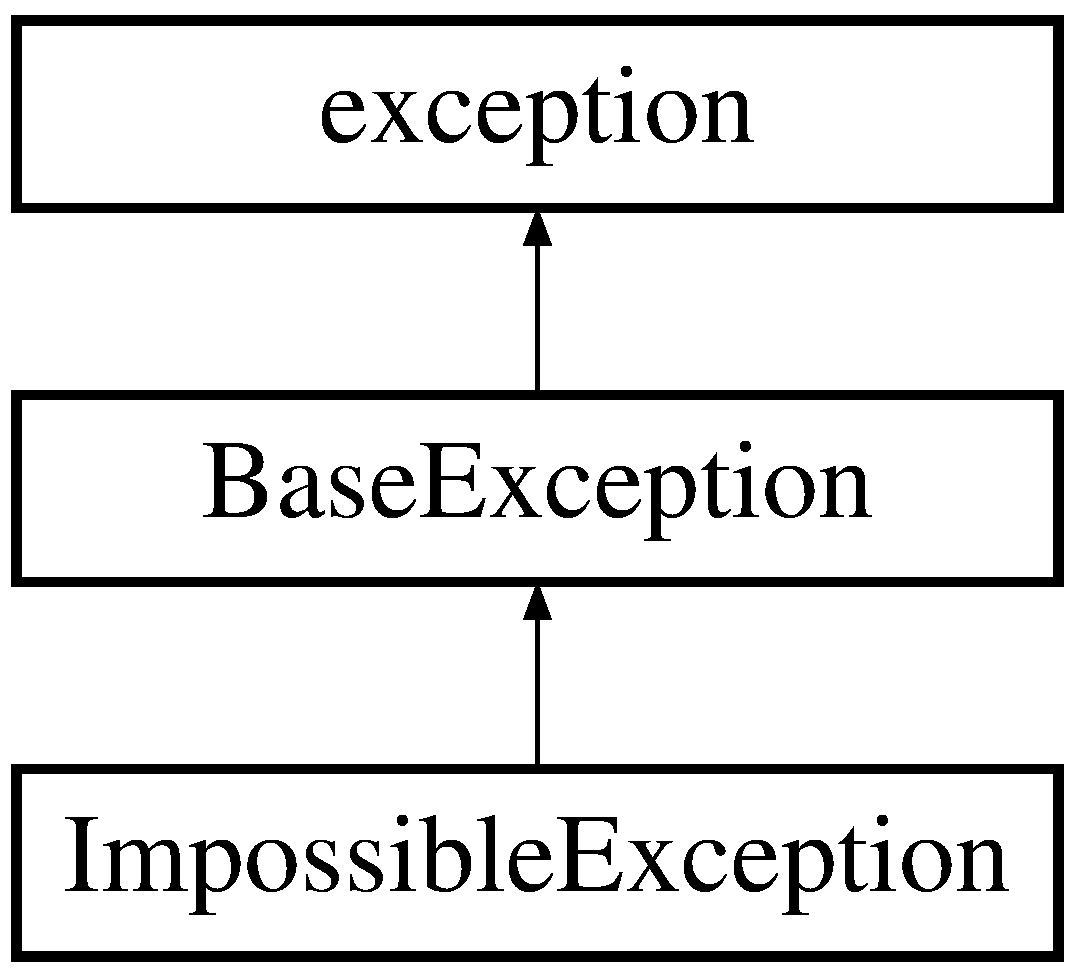
\includegraphics[height=3.000000cm]{class_impossible_exception}
\end{center}
\end{figure}
\subsection*{Public Member Functions}
\begin{DoxyCompactItemize}
\item 
\hypertarget{class_impossible_exception_a88afecc506123920b1bcd8f8b1bc612d}{{\bfseries Impossible\-Exception} (const std\-::string \&msg)}\label{class_impossible_exception_a88afecc506123920b1bcd8f8b1bc612d}

\item 
\hypertarget{class_impossible_exception_a3368d553e27e69451266f56bc37e9a86}{virtual const char $\ast$ {\bfseries what} () const noexcept}\label{class_impossible_exception_a3368d553e27e69451266f56bc37e9a86}

\end{DoxyCompactItemize}


\subsection{Detailed Description}


Definition at line 12 of file impossible\-\_\-exception.\-h.



The documentation for this class was generated from the following files\-:\begin{DoxyCompactItemize}
\item 
/home/travis/build/tomas789/tonav/include/exceptions/impossible\-\_\-exception.\-h\item 
/home/travis/build/tomas789/tonav/src/exceptions/impossible\-\_\-exception.\-cpp\end{DoxyCompactItemize}

\hypertarget{class_imu_buffer}{\section{Imu\-Buffer Class Reference}
\label{class_imu_buffer}\index{Imu\-Buffer@{Imu\-Buffer}}
}


Buffer of I\-M\-U data measurements.  




{\ttfamily \#include $<$imu\-\_\-buffer.\-h$>$}

\subsection*{Public Member Functions}
\begin{DoxyCompactItemize}
\item 
\hypertarget{class_imu_buffer_a50dd06412b4e7f3f041ae6ab6fa680b0}{{\bfseries Imu\-Buffer} (Imu\-Device device, std\-::size\-\_\-t size)}\label{class_imu_buffer_a50dd06412b4e7f3f041ae6ab6fa680b0}

\item 
\hypertarget{class_imu_buffer_a03aff5b4ab113232a3fa032115249018}{void {\bfseries add\-Measurement} (\hyperlink{class_imu_item}{Imu\-Item} item)}\label{class_imu_buffer_a03aff5b4ab113232a3fa032115249018}

\item 
\hypertarget{class_imu_buffer_a70e3b571c1ff9c9e2ca60c8dfd1eee1c}{\hyperlink{class_imu_item}{Imu\-Item} {\bfseries interpolate\-At\-Time} (double time) const }\label{class_imu_buffer_a70e3b571c1ff9c9e2ca60c8dfd1eee1c}

\item 
\hypertarget{class_imu_buffer_a3c23315625f26a5673b814f513c1bc98}{double {\bfseries get\-Min\-Time} () const }\label{class_imu_buffer_a3c23315625f26a5673b814f513c1bc98}

\item 
\hypertarget{class_imu_buffer_aa3f3a11dc21d97386b3154122cb8e296}{double {\bfseries get\-Max\-Time} () const }\label{class_imu_buffer_aa3f3a11dc21d97386b3154122cb8e296}

\item 
\hypertarget{class_imu_buffer_a4500c72f04ac02e629e77762953c6abc}{bool {\bfseries is\-Ready} () const }\label{class_imu_buffer_a4500c72f04ac02e629e77762953c6abc}

\end{DoxyCompactItemize}


\subsection{Detailed Description}
Buffer of I\-M\-U data measurements. 

\begin{DoxyRefDesc}{Deprecated}
\item[\hyperlink{deprecated__deprecated000002}{Deprecated}]This class is no longer needed. It is used in \hyperlink{class_navigator}{Navigator} class only.\end{DoxyRefDesc}


Using this class you can interpolate I\-M\-U measurement at any time in interval \mbox{[}get\-Min\-Time(), get\-Max\-Time()\mbox{]} 

Definition at line 22 of file imu\-\_\-buffer.\-h.



The documentation for this class was generated from the following files\-:\begin{DoxyCompactItemize}
\item 
/home/travis/build/tomas789/tonav/include/imu\-\_\-buffer.\-h\item 
/home/travis/build/tomas789/tonav/src/imu\-\_\-buffer.\-cpp\end{DoxyCompactItemize}

\hypertarget{classmsckf_1_1_imu_buffer}{\section{msckf.\-Imu\-Buffer Class Reference}
\label{classmsckf_1_1_imu_buffer}\index{msckf.\-Imu\-Buffer@{msckf.\-Imu\-Buffer}}
}
\subsection*{Public Member Functions}
\begin{DoxyCompactItemize}
\item 
\hypertarget{classmsckf_1_1_imu_buffer_a6a576e23425beb88711a0b6c9fd00d6e}{def {\bfseries \-\_\-\-\_\-init\-\_\-\-\_\-}}\label{classmsckf_1_1_imu_buffer_a6a576e23425beb88711a0b6c9fd00d6e}

\item 
\hypertarget{classmsckf_1_1_imu_buffer_a93afe342c8d427e7a7c9bd2f1964308b}{def {\bfseries push}}\label{classmsckf_1_1_imu_buffer_a93afe342c8d427e7a7c9bd2f1964308b}

\item 
\hypertarget{classmsckf_1_1_imu_buffer_a698da50c389659d3c762ddc2251296e3}{def {\bfseries check\-\_\-integrity}}\label{classmsckf_1_1_imu_buffer_a698da50c389659d3c762ddc2251296e3}

\item 
\hypertarget{classmsckf_1_1_imu_buffer_a359f10c40136ea9c4e75c6c3cb2f4310}{def {\bfseries min}}\label{classmsckf_1_1_imu_buffer_a359f10c40136ea9c4e75c6c3cb2f4310}

\item 
\hypertarget{classmsckf_1_1_imu_buffer_adb77be97e9cfe0e5a3e58c607c9dfebe}{def {\bfseries max}}\label{classmsckf_1_1_imu_buffer_adb77be97e9cfe0e5a3e58c607c9dfebe}

\item 
\hypertarget{classmsckf_1_1_imu_buffer_ab0e45309457a41cad3d1783e45c43830}{def {\bfseries mean\-\_\-value}}\label{classmsckf_1_1_imu_buffer_ab0e45309457a41cad3d1783e45c43830}

\item 
\hypertarget{classmsckf_1_1_imu_buffer_a747a692ef45bcb6b4c2736e34900453d}{def {\bfseries \-\_\-\-\_\-len\-\_\-\-\_\-}}\label{classmsckf_1_1_imu_buffer_a747a692ef45bcb6b4c2736e34900453d}

\item 
\hypertarget{classmsckf_1_1_imu_buffer_a368b04188fcaaaf0fea135d733618edb}{def {\bfseries \-\_\-\-\_\-getitem\-\_\-\-\_\-}}\label{classmsckf_1_1_imu_buffer_a368b04188fcaaaf0fea135d733618edb}

\item 
\hypertarget{classmsckf_1_1_imu_buffer_ad767ec99d974d97547882580f9817698}{def {\bfseries pop\-\_\-min}}\label{classmsckf_1_1_imu_buffer_ad767ec99d974d97547882580f9817698}

\item 
\hypertarget{classmsckf_1_1_imu_buffer_aa10df9ce04292c14a6d6ff9ee0b1921d}{def {\bfseries interpolate}}\label{classmsckf_1_1_imu_buffer_aa10df9ce04292c14a6d6ff9ee0b1921d}

\end{DoxyCompactItemize}
\subsection*{Public Attributes}
\begin{DoxyCompactItemize}
\item 
\hypertarget{classmsckf_1_1_imu_buffer_a32ca4fadfb0ea149595c2e525359dfd1}{{\bfseries device}}\label{classmsckf_1_1_imu_buffer_a32ca4fadfb0ea149595c2e525359dfd1}

\item 
\hypertarget{classmsckf_1_1_imu_buffer_a30ea8b12a07b5f7e594867741dcae9b7}{{\bfseries items}}\label{classmsckf_1_1_imu_buffer_a30ea8b12a07b5f7e594867741dcae9b7}

\end{DoxyCompactItemize}


\subsection{Detailed Description}
\begin{DoxyVerb}Contains a list of IMU measurements. Times are unique.
\end{DoxyVerb}
 

Definition at line 155 of file msckf.\-py.



The documentation for this class was generated from the following file\-:\begin{DoxyCompactItemize}
\item 
/home/travis/build/tomas789/tonav/prototype/msckf.\-py\end{DoxyCompactItemize}

\hypertarget{classmsckf_1_1_imu_device}{\section{msckf.\-Imu\-Device Class Reference}
\label{classmsckf_1_1_imu_device}\index{msckf.\-Imu\-Device@{msckf.\-Imu\-Device}}
}
Inheritance diagram for msckf.\-Imu\-Device\-:\begin{figure}[H]
\begin{center}
\leavevmode
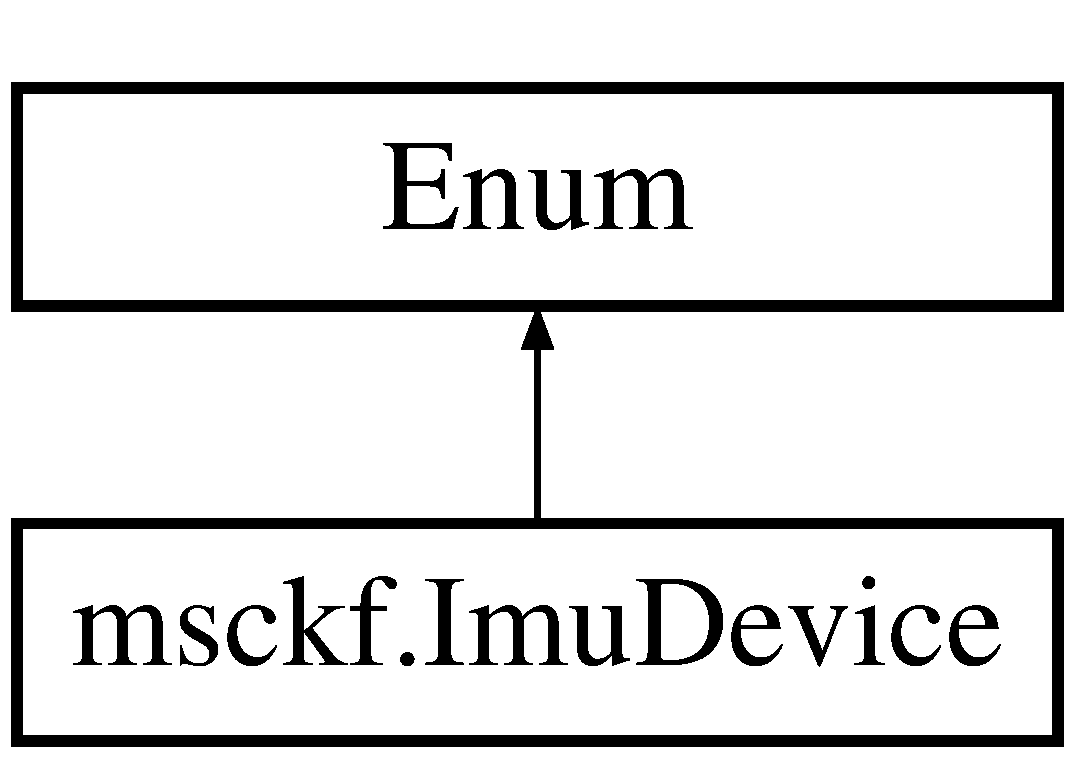
\includegraphics[height=2.000000cm]{classmsckf_1_1_imu_device}
\end{center}
\end{figure}
\subsection*{Static Public Attributes}
\begin{DoxyCompactItemize}
\item 
\hypertarget{classmsckf_1_1_imu_device_a3faeff4eaaf36e190287606fae61079f}{int {\bfseries accelerometer} = 1}\label{classmsckf_1_1_imu_device_a3faeff4eaaf36e190287606fae61079f}

\item 
\hypertarget{classmsckf_1_1_imu_device_acad284d6013b952fdd878b8a768e7169}{int {\bfseries gyroscope} = 2}\label{classmsckf_1_1_imu_device_acad284d6013b952fdd878b8a768e7169}

\end{DoxyCompactItemize}


\subsection{Detailed Description}


Definition at line 97 of file msckf.\-py.



The documentation for this class was generated from the following file\-:\begin{DoxyCompactItemize}
\item 
/home/travis/build/tomas789/tonav/prototype/msckf.\-py\end{DoxyCompactItemize}

\hypertarget{class_imu_feed}{\section{Imu\-Feed Class Reference}
\label{class_imu_feed}\index{Imu\-Feed@{Imu\-Feed}}
}
\subsection*{Public Member Functions}
\begin{DoxyCompactItemize}
\item 
\hypertarget{class_imu_feed_a5ab48b9002ee9eacfe760afc579e1b50}{bool {\bfseries has\-Next} () const }\label{class_imu_feed_a5ab48b9002ee9eacfe760afc579e1b50}

\item 
\hypertarget{class_imu_feed_ab36b0a9833d5687820065483818de270}{void {\bfseries next} ()}\label{class_imu_feed_ab36b0a9833d5687820065483818de270}

\item 
\hypertarget{class_imu_feed_a48e5bf07fb20dc5f55e3078b6c57adc2}{const \hyperlink{class_imu_item}{Imu\-Item} \& {\bfseries top} () const }\label{class_imu_feed_a48e5bf07fb20dc5f55e3078b6c57adc2}

\end{DoxyCompactItemize}
\subsection*{Static Public Member Functions}
\begin{DoxyCompactItemize}
\item 
\hypertarget{class_imu_feed_a65c5b70f27e938f6a13bd55fd0bb5127}{static \hyperlink{class_imu_feed}{Imu\-Feed} {\bfseries from\-Dataset} (boost\-::filesystem\-::path path)}\label{class_imu_feed_a65c5b70f27e938f6a13bd55fd0bb5127}

\end{DoxyCompactItemize}


\subsection{Detailed Description}


Definition at line 14 of file imu\-\_\-feed.\-h.



The documentation for this class was generated from the following files\-:\begin{DoxyCompactItemize}
\item 
/home/travis/build/tomas789/tonav/include/imu\-\_\-feed.\-h\item 
/home/travis/build/tomas789/tonav/src/imu\-\_\-feed.\-cpp\end{DoxyCompactItemize}

\hypertarget{class_imu_item}{\section{Imu\-Item Class Reference}
\label{class_imu_item}\index{Imu\-Item@{Imu\-Item}}
}
\subsection*{Public Member Functions}
\begin{DoxyCompactItemize}
\item 
\hypertarget{class_imu_item_ac12a9c7f77a7318de5893a26284c8f12}{Imu\-Device {\bfseries get\-Device} () const }\label{class_imu_item_ac12a9c7f77a7318de5893a26284c8f12}

\item 
\hypertarget{class_imu_item_adf0603391765e4950651ee67fe2273b7}{double {\bfseries get\-Time} () const }\label{class_imu_item_adf0603391765e4950651ee67fe2273b7}

\item 
\hypertarget{class_imu_item_a9fe54cf71ea23dc3f044bf849a50743b}{double {\bfseries get\-X} () const }\label{class_imu_item_a9fe54cf71ea23dc3f044bf849a50743b}

\item 
\hypertarget{class_imu_item_af969726f713eb67b6b544133bea5fd21}{double {\bfseries get\-Y} () const }\label{class_imu_item_af969726f713eb67b6b544133bea5fd21}

\item 
\hypertarget{class_imu_item_af010fd2fd5ecd5868764a760f6040af5}{double {\bfseries get\-Z} () const }\label{class_imu_item_af010fd2fd5ecd5868764a760f6040af5}

\item 
\hypertarget{class_imu_item_a1cd4668ce368cb3b8360f42a1ab97580}{Eigen\-::\-Vector3d {\bfseries get\-Vector} () const }\label{class_imu_item_a1cd4668ce368cb3b8360f42a1ab97580}

\end{DoxyCompactItemize}
\subsection*{Static Public Member Functions}
\begin{DoxyCompactItemize}
\item 
\hypertarget{class_imu_item_af127ca299205f31693ed6a85330bf915}{static \hyperlink{class_imu_item}{Imu\-Item} {\bfseries from\-String} (std\-::string line)}\label{class_imu_item_af127ca299205f31693ed6a85330bf915}

\item 
\hypertarget{class_imu_item_a0a28edeccaf5f42fabf05e76c5c46519}{static \hyperlink{class_imu_item}{Imu\-Item} {\bfseries from\-Vector3d} (double time, const Imu\-Device \&device, const Eigen\-::\-Vector3d \&data)}\label{class_imu_item_a0a28edeccaf5f42fabf05e76c5c46519}

\end{DoxyCompactItemize}
\subsection*{Friends}
\begin{DoxyCompactItemize}
\item 
\hypertarget{class_imu_item_affcdaeabb9b33248d9efdf687f2eab5c}{class {\bfseries Imu\-Buffer}}\label{class_imu_item_affcdaeabb9b33248d9efdf687f2eab5c}

\end{DoxyCompactItemize}


\subsection{Detailed Description}


Definition at line 15 of file imu\-\_\-item.\-h.



The documentation for this class was generated from the following files\-:\begin{DoxyCompactItemize}
\item 
/home/tomaskrejci/catkin\-\_\-ws/src/tonav/include/imu\-\_\-item.\-h\item 
/home/tomaskrejci/catkin\-\_\-ws/src/tonav/src/imu\-\_\-item.\-cpp\end{DoxyCompactItemize}

\hypertarget{classmsckf_1_1_imu_item}{\section{msckf.\-Imu\-Item Class Reference}
\label{classmsckf_1_1_imu_item}\index{msckf.\-Imu\-Item@{msckf.\-Imu\-Item}}
}
\subsection*{Public Member Functions}
\begin{DoxyCompactItemize}
\item 
\hypertarget{classmsckf_1_1_imu_item_a0a4c7f19f46f237e89669fa8c9ea43b1}{def {\bfseries \-\_\-\-\_\-init\-\_\-\-\_\-}}\label{classmsckf_1_1_imu_item_a0a4c7f19f46f237e89669fa8c9ea43b1}

\item 
\hypertarget{classmsckf_1_1_imu_item_ae408089f0f3b7be27c0e951ebd5e2190}{def {\bfseries \-\_\-\-\_\-lt\-\_\-\-\_\-}}\label{classmsckf_1_1_imu_item_ae408089f0f3b7be27c0e951ebd5e2190}

\item 
\hypertarget{classmsckf_1_1_imu_item_a1142bdc6e7dc7a06bc16f6e359d0bb22}{def {\bfseries \-\_\-\-\_\-le\-\_\-\-\_\-}}\label{classmsckf_1_1_imu_item_a1142bdc6e7dc7a06bc16f6e359d0bb22}

\item 
\hypertarget{classmsckf_1_1_imu_item_abeeeda7fc9045aecfa4d700ec406d266}{def {\bfseries \-\_\-\-\_\-gt\-\_\-\-\_\-}}\label{classmsckf_1_1_imu_item_abeeeda7fc9045aecfa4d700ec406d266}

\item 
\hypertarget{classmsckf_1_1_imu_item_aef7d5c469fd651c4542dfc9552388a07}{def {\bfseries \-\_\-\-\_\-ge\-\_\-\-\_\-}}\label{classmsckf_1_1_imu_item_aef7d5c469fd651c4542dfc9552388a07}

\item 
\hypertarget{classmsckf_1_1_imu_item_a6acb545776a9fa7398760405c6d79c1a}{def {\bfseries \-\_\-\-\_\-eq\-\_\-\-\_\-}}\label{classmsckf_1_1_imu_item_a6acb545776a9fa7398760405c6d79c1a}

\item 
\hypertarget{classmsckf_1_1_imu_item_a70a0dfe1b2fcbf6eed7282e3bea63271}{def {\bfseries \-\_\-\-\_\-ne\-\_\-\-\_\-}}\label{classmsckf_1_1_imu_item_a70a0dfe1b2fcbf6eed7282e3bea63271}

\item 
\hypertarget{classmsckf_1_1_imu_item_a8546cab5c7c0821391278c48fda88fb3}{def {\bfseries device}}\label{classmsckf_1_1_imu_item_a8546cab5c7c0821391278c48fda88fb3}

\item 
\hypertarget{classmsckf_1_1_imu_item_af1453674ea9cba40874df29d17621796}{def {\bfseries time}}\label{classmsckf_1_1_imu_item_af1453674ea9cba40874df29d17621796}

\item 
\hypertarget{classmsckf_1_1_imu_item_a70dbde6767fb3a7adebb1a6af0626aec}{def {\bfseries value}}\label{classmsckf_1_1_imu_item_a70dbde6767fb3a7adebb1a6af0626aec}

\end{DoxyCompactItemize}


\subsection{Detailed Description}


Definition at line 102 of file msckf.\-py.



The documentation for this class was generated from the following file\-:\begin{DoxyCompactItemize}
\item 
/home/travis/build/tomas789/tonav/prototype/msckf.\-py\end{DoxyCompactItemize}

\hypertarget{classmsckf_1_1_msckf}{\section{msckf.\-Msckf Class Reference}
\label{classmsckf_1_1_msckf}\index{msckf.\-Msckf@{msckf.\-Msckf}}
}
\subsection*{Public Member Functions}
\begin{DoxyCompactItemize}
\item 
\hypertarget{classmsckf_1_1_msckf_acece06247a28c9c6cc17228a7471281e}{def {\bfseries \-\_\-\-\_\-init\-\_\-\-\_\-}}\label{classmsckf_1_1_msckf_acece06247a28c9c6cc17228a7471281e}

\item 
\hypertarget{classmsckf_1_1_msckf_ab718a75ae92fe78165b104903589996b}{def {\bfseries callback\-\_\-imu}}\label{classmsckf_1_1_msckf_ab718a75ae92fe78165b104903589996b}

\item 
\hypertarget{classmsckf_1_1_msckf_ae226b29e88715596bea9912fa5b9eef9}{def {\bfseries process\-\_\-imu}}\label{classmsckf_1_1_msckf_ae226b29e88715596bea9912fa5b9eef9}

\item 
\hypertarget{classmsckf_1_1_msckf_a1489f7f6eb9ac6b0478a186fcd05650f}{def {\bfseries callback\-\_\-camera}}\label{classmsckf_1_1_msckf_a1489f7f6eb9ac6b0478a186fcd05650f}

\item 
\hypertarget{classmsckf_1_1_msckf_abb3ef8cce650ce56470f7f2d23e793c2}{def {\bfseries try\-\_\-initialize}}\label{classmsckf_1_1_msckf_abb3ef8cce650ce56470f7f2d23e793c2}

\item 
\hypertarget{classmsckf_1_1_msckf_ac9935613a6c0603529dc051505c19f63}{def {\bfseries try\-\_\-steps}}\label{classmsckf_1_1_msckf_ac9935613a6c0603529dc051505c19f63}

\item 
\hypertarget{classmsckf_1_1_msckf_a5f8d7a1f9f02faaa3ce4dcf23e7024ff}{def {\bfseries propagate\-\_\-up\-\_\-to\-\_\-time\-\_\-incl}}\label{classmsckf_1_1_msckf_a5f8d7a1f9f02faaa3ce4dcf23e7024ff}

\item 
\hypertarget{classmsckf_1_1_msckf_a2a9394d1a3c7220d2804cbb6ca103b4f}{def {\bfseries update}}\label{classmsckf_1_1_msckf_a2a9394d1a3c7220d2804cbb6ca103b4f}

\item 
\hypertarget{classmsckf_1_1_msckf_a48162eab93295a3aa9827d02570ecdf3}{def {\bfseries triangulate}}\label{classmsckf_1_1_msckf_a48162eab93295a3aa9827d02570ecdf3}

\item 
\hypertarget{classmsckf_1_1_msckf_a091abe4b54b43f7d11e1ffe2063f7ac9}{def {\bfseries h}}\label{classmsckf_1_1_msckf_a091abe4b54b43f7d11e1ffe2063f7ac9}

\item 
\hypertarget{classmsckf_1_1_msckf_aa923443e7b9f8c18963493b1a910025e}{def {\bfseries g}}\label{classmsckf_1_1_msckf_aa923443e7b9f8c18963493b1a910025e}

\item 
\hypertarget{classmsckf_1_1_msckf_a561f373b33a2c3b7e8b9d6e1e8c95328}{def {\bfseries feature\-\_\-residual}}\label{classmsckf_1_1_msckf_a561f373b33a2c3b7e8b9d6e1e8c95328}

\item 
\hypertarget{classmsckf_1_1_msckf_a67a09f9f462392f3bb707ac698b6ed0e}{def {\bfseries camera\-\_\-jacobian}}\label{classmsckf_1_1_msckf_a67a09f9f462392f3bb707ac698b6ed0e}

\item 
\hypertarget{classmsckf_1_1_msckf_a59f002d186ffda17b1a1dcc8d2a723de}{def {\bfseries compute\-\_\-global\-\_\-feature\-\_\-estimate}}\label{classmsckf_1_1_msckf_a59f002d186ffda17b1a1dcc8d2a723de}

\item 
\hypertarget{classmsckf_1_1_msckf_a45893991d0f6af50e0eb902c6416b623}{def {\bfseries calculate\-\_\-camera\-\_\-projection\-\_\-estimate}}\label{classmsckf_1_1_msckf_a45893991d0f6af50e0eb902c6416b623}

\item 
\hypertarget{classmsckf_1_1_msckf_a0868335826b7b55548236cd06e7a248c}{def {\bfseries pinhole\-\_\-model}}\label{classmsckf_1_1_msckf_a0868335826b7b55548236cd06e7a248c}

\item 
\hypertarget{classmsckf_1_1_msckf_a18e2cb57b56fdc5f7d66b8e36cc067ce}{def {\bfseries interpolate}}\label{classmsckf_1_1_msckf_a18e2cb57b56fdc5f7d66b8e36cc067ce}

\item 
\hypertarget{classmsckf_1_1_msckf_acf89b57822a098ee1a650849a37361eb}{def {\bfseries publish\-\_\-localization}}\label{classmsckf_1_1_msckf_acf89b57822a098ee1a650849a37361eb}

\item 
\hypertarget{classmsckf_1_1_msckf_ab55273376c5e47b07ba919d6486a40b2}{def {\bfseries publish\-\_\-image\-\_\-if\-\_\-new\-\_\-available}}\label{classmsckf_1_1_msckf_ab55273376c5e47b07ba919d6486a40b2}

\item 
\hypertarget{classmsckf_1_1_msckf_a72c2622b8dec25f90ecca34bd759e8af}{def {\bfseries run}}\label{classmsckf_1_1_msckf_a72c2622b8dec25f90ecca34bd759e8af}

\end{DoxyCompactItemize}
\subsection*{Public Attributes}
\begin{DoxyCompactItemize}
\item 
\hypertarget{classmsckf_1_1_msckf_aa293c70761d866bcdf8e984a1385de64}{{\bfseries imu\-\_\-subscriber}}\label{classmsckf_1_1_msckf_aa293c70761d866bcdf8e984a1385de64}

\item 
\hypertarget{classmsckf_1_1_msckf_a354aa0dd7846a4787802bf3bb7791173}{{\bfseries camera\-\_\-subscriber}}\label{classmsckf_1_1_msckf_a354aa0dd7846a4787802bf3bb7791173}

\item 
\hypertarget{classmsckf_1_1_msckf_a105ff6012b0df8b799c2be6ab9c76add}{{\bfseries pointcloud\-\_\-publisher}}\label{classmsckf_1_1_msckf_a105ff6012b0df8b799c2be6ab9c76add}

\item 
\hypertarget{classmsckf_1_1_msckf_aa175e86a112bcc920bd6b8cf54083e86}{{\bfseries br}}\label{classmsckf_1_1_msckf_aa175e86a112bcc920bd6b8cf54083e86}

\item 
\hypertarget{classmsckf_1_1_msckf_a5ac0c36ef36e91f2b3a8847145d6e56a}{{\bfseries lock}}\label{classmsckf_1_1_msckf_a5ac0c36ef36e91f2b3a8847145d6e56a}

\item 
\hypertarget{classmsckf_1_1_msckf_a65e9d1ff1559e16bd18e01212b428252}{{\bfseries listener}}\label{classmsckf_1_1_msckf_a65e9d1ff1559e16bd18e01212b428252}

\item 
\hypertarget{classmsckf_1_1_msckf_abe179b3b52794f6c5d4a9598f1286126}{{\bfseries cam\-\_\-to\-\_\-process}}\label{classmsckf_1_1_msckf_abe179b3b52794f6c5d4a9598f1286126}

\item 
\hypertarget{classmsckf_1_1_msckf_a787a99dcc98a91e5a571f4e313a96b36}{{\bfseries state}}\label{classmsckf_1_1_msckf_a787a99dcc98a91e5a571f4e313a96b36}

\item 
\hypertarget{classmsckf_1_1_msckf_a14270fb94fe42ea7b3c7238afae4ef22}{{\bfseries image\-\_\-tracker}}\label{classmsckf_1_1_msckf_a14270fb94fe42ea7b3c7238afae4ef22}

\item 
\hypertarget{classmsckf_1_1_msckf_aa3d7e17f0521408497a79c47039bcdb9}{{\bfseries bridge}}\label{classmsckf_1_1_msckf_aa3d7e17f0521408497a79c47039bcdb9}

\item 
\hypertarget{classmsckf_1_1_msckf_a9ac9d9d8888316a8b2ebf1b446f17e07}{{\bfseries cam\-\_\-poses}}\label{classmsckf_1_1_msckf_a9ac9d9d8888316a8b2ebf1b446f17e07}

\item 
\hypertarget{classmsckf_1_1_msckf_ae967978398f1652655b0ad7edd0f9af1}{{\bfseries buffer\-\_\-size\-\_\-to\-\_\-initialize}}\label{classmsckf_1_1_msckf_ae967978398f1652655b0ad7edd0f9af1}

\item 
\hypertarget{classmsckf_1_1_msckf_a8f68a433bdc94aa74889d127d9e91f31}{{\bfseries image\-\_\-rows}}\label{classmsckf_1_1_msckf_a8f68a433bdc94aa74889d127d9e91f31}

\item 
\hypertarget{classmsckf_1_1_msckf_a6e69e72653d9941528a1e4cecbc16371}{{\bfseries buffers}}\label{classmsckf_1_1_msckf_a6e69e72653d9941528a1e4cecbc16371}

\item 
\hypertarget{classmsckf_1_1_msckf_a2e46d6304ad2781ab231eb5cbaa935a0}{{\bfseries t\-\_\-d}}\label{classmsckf_1_1_msckf_a2e46d6304ad2781ab231eb5cbaa935a0}

\item 
\hypertarget{classmsckf_1_1_msckf_af788a1595dc960d3f58cc28ba33228d4}{{\bfseries t\-\_\-r}}\label{classmsckf_1_1_msckf_af788a1595dc960d3f58cc28ba33228d4}

\item 
\hypertarget{classmsckf_1_1_msckf_a8456c22259389af1d92a3926e7b7020e}{{\bfseries image\-\_\-publisher}}\label{classmsckf_1_1_msckf_a8456c22259389af1d92a3926e7b7020e}

\item 
\hypertarget{classmsckf_1_1_msckf_af1c0cd63952b6bd0ae751c39c4e6422a}{{\bfseries tf\-Buffer}}\label{classmsckf_1_1_msckf_af1c0cd63952b6bd0ae751c39c4e6422a}

\end{DoxyCompactItemize}


\subsection{Detailed Description}


Definition at line 575 of file msckf.\-py.



The documentation for this class was generated from the following file\-:\begin{DoxyCompactItemize}
\item 
/home/travis/build/tomas789/tonav/prototype/msckf.\-py\end{DoxyCompactItemize}

\hypertarget{class_navigator}{\section{Navigator Class Reference}
\label{class_navigator}\index{Navigator@{Navigator}}
}


Perform navigation from dataset.  




{\ttfamily \#include $<$navigator.\-h$>$}

\subsection*{Public Member Functions}
\begin{DoxyCompactItemize}
\item 
int \hyperlink{class_navigator_a614e53f6cf6859608b14057272003cea}{run} (int argc, const char $\ast$argv\mbox{[}$\,$\mbox{]})
\begin{DoxyCompactList}\small\item\em Run navigation node from dataset. \end{DoxyCompactList}\end{DoxyCompactItemize}


\subsection{Detailed Description}
Perform navigation from dataset. 

\begin{DoxyRefDesc}{Deprecated}
\item[\hyperlink{deprecated__deprecated000003}{Deprecated}]This is deprecated. Use \hyperlink{class_tonav}{Tonav} or it's convenience wrapper \hyperlink{class_tonav_ros}{Tonav\-Ros} instead. \end{DoxyRefDesc}


Definition at line 16 of file navigator.\-h.



\subsection{Member Function Documentation}
\hypertarget{class_navigator_a614e53f6cf6859608b14057272003cea}{\index{Navigator@{Navigator}!run@{run}}
\index{run@{run}!Navigator@{Navigator}}
\subsubsection[{run}]{\setlength{\rightskip}{0pt plus 5cm}int Navigator\-::run (
\begin{DoxyParamCaption}
\item[{int}]{argc, }
\item[{const char $\ast$}]{argv\mbox{[}$\,$\mbox{]}}
\end{DoxyParamCaption}
)}}\label{class_navigator_a614e53f6cf6859608b14057272003cea}


Run navigation node from dataset. 

\begin{DoxyRefDesc}{Deprecated}
\item[\hyperlink{deprecated__deprecated000004}{Deprecated}]This is deprecated. Use \hyperlink{class_tonav}{Tonav} or it's convenience wrapper \hyperlink{class_tonav_ros}{Tonav\-Ros} instead.\end{DoxyRefDesc}



\begin{DoxyParams}{Parameters}
{\em argc} & Number of command line arguments. \\
\hline
{\em argv} & List of command line arguments. \\
\hline
\end{DoxyParams}


Definition at line 27 of file navigator.\-cpp.



The documentation for this class was generated from the following files\-:\begin{DoxyCompactItemize}
\item 
/home/travis/build/tomas789/tonav/include/navigator.\-h\item 
/home/travis/build/tomas789/tonav/src/navigator.\-cpp\end{DoxyCompactItemize}

\hypertarget{classmsckf_1_1_pose_get}{\section{msckf.\-Pose\-Get Class Reference}
\label{classmsckf_1_1_pose_get}\index{msckf.\-Pose\-Get@{msckf.\-Pose\-Get}}
}
\subsection*{Public Member Functions}
\begin{DoxyCompactItemize}
\item 
\hypertarget{classmsckf_1_1_pose_get_a3a5b9917934e12b4d6a98a95f87db759}{def {\bfseries \-\_\-\-\_\-init\-\_\-\-\_\-}}\label{classmsckf_1_1_pose_get_a3a5b9917934e12b4d6a98a95f87db759}

\item 
\hypertarget{classmsckf_1_1_pose_get_aa67fbb72a16db07345b41a2d4ca6e9f6}{def {\bfseries \-\_\-\-\_\-getitem\-\_\-\-\_\-}}\label{classmsckf_1_1_pose_get_aa67fbb72a16db07345b41a2d4ca6e9f6}

\end{DoxyCompactItemize}
\subsection*{Public Attributes}
\begin{DoxyCompactItemize}
\item 
\hypertarget{classmsckf_1_1_pose_get_a75b39f2276ee24bc71dbbd5ce43ec585}{{\bfseries state}}\label{classmsckf_1_1_pose_get_a75b39f2276ee24bc71dbbd5ce43ec585}

\end{DoxyCompactItemize}


\subsection{Detailed Description}


Definition at line 230 of file msckf.\-py.



The documentation for this class was generated from the following file\-:\begin{DoxyCompactItemize}
\item 
/home/travis/build/tomas789/tonav/prototype/msckf.\-py\end{DoxyCompactItemize}

\hypertarget{classimage__transport_1_1_publisher}{\section{image\-\_\-transport\-:\-:Publisher Class Reference}
\label{classimage__transport_1_1_publisher}\index{image\-\_\-transport\-::\-Publisher@{image\-\_\-transport\-::\-Publisher}}
}


Manages advertisements of multiple transport options on an Image topic.  




{\ttfamily \#include $<$publisher.\-h$>$}

\subsection*{Classes}
\begin{DoxyCompactItemize}
\item 
struct \hyperlink{structimage__transport_1_1_publisher_1_1_impl}{Impl}
\end{DoxyCompactItemize}
\subsection*{Public Member Functions}
\begin{DoxyCompactItemize}
\item 
uint32\-\_\-t \hyperlink{classimage__transport_1_1_publisher_ac88d47f80afa429ea135f5bca7448dd9}{get\-Num\-Subscribers} () const 
\begin{DoxyCompactList}\small\item\em Returns the number of subscribers that are currently connected to this \hyperlink{classimage__transport_1_1_publisher}{Publisher}. \end{DoxyCompactList}\item 
\hypertarget{classimage__transport_1_1_publisher_a9c76ade4e9217ba84b4c5e8f71041a39}{std\-::string \hyperlink{classimage__transport_1_1_publisher_a9c76ade4e9217ba84b4c5e8f71041a39}{get\-Topic} () const }\label{classimage__transport_1_1_publisher_a9c76ade4e9217ba84b4c5e8f71041a39}

\begin{DoxyCompactList}\small\item\em Returns the base topic of this \hyperlink{classimage__transport_1_1_publisher}{Publisher}. \end{DoxyCompactList}\item 
\hypertarget{classimage__transport_1_1_publisher_adca2507fe8999ccfdfc6d8871f986e10}{void \hyperlink{classimage__transport_1_1_publisher_adca2507fe8999ccfdfc6d8871f986e10}{publish} (const sensor\-\_\-msgs\-::\-Image \&message) const }\label{classimage__transport_1_1_publisher_adca2507fe8999ccfdfc6d8871f986e10}

\begin{DoxyCompactList}\small\item\em Publish an image on the topics associated with this \hyperlink{classimage__transport_1_1_publisher}{Publisher}. \end{DoxyCompactList}\item 
\hypertarget{classimage__transport_1_1_publisher_aa707c681bc6760150aca17d25f532113}{void \hyperlink{classimage__transport_1_1_publisher_aa707c681bc6760150aca17d25f532113}{publish} (const sensor\-\_\-msgs\-::\-Image\-Const\-Ptr \&message) const }\label{classimage__transport_1_1_publisher_aa707c681bc6760150aca17d25f532113}

\begin{DoxyCompactList}\small\item\em Publish an image on the topics associated with this \hyperlink{classimage__transport_1_1_publisher}{Publisher}. \end{DoxyCompactList}\item 
\hypertarget{classimage__transport_1_1_publisher_a072fafb7790734db8ecda3c6704b9396}{void \hyperlink{classimage__transport_1_1_publisher_a072fafb7790734db8ecda3c6704b9396}{shutdown} ()}\label{classimage__transport_1_1_publisher_a072fafb7790734db8ecda3c6704b9396}

\begin{DoxyCompactList}\small\item\em Shutdown the advertisements associated with this \hyperlink{classimage__transport_1_1_publisher}{Publisher}. \end{DoxyCompactList}\item 
\hypertarget{classimage__transport_1_1_publisher_abebb98c83a1d185504a528e46011ad5e}{{\bfseries operator void $\ast$} () const }\label{classimage__transport_1_1_publisher_abebb98c83a1d185504a528e46011ad5e}

\item 
\hypertarget{classimage__transport_1_1_publisher_a48f65b298d5f1127fcf5c0ff44ee23c1}{bool {\bfseries operator$<$} (const \hyperlink{classimage__transport_1_1_publisher}{Publisher} \&rhs) const }\label{classimage__transport_1_1_publisher_a48f65b298d5f1127fcf5c0ff44ee23c1}

\item 
\hypertarget{classimage__transport_1_1_publisher_a10b1cdd3affd8816707c7f4d14b9c2be}{bool {\bfseries operator!=} (const \hyperlink{classimage__transport_1_1_publisher}{Publisher} \&rhs) const }\label{classimage__transport_1_1_publisher_a10b1cdd3affd8816707c7f4d14b9c2be}

\item 
\hypertarget{classimage__transport_1_1_publisher_af152f8ef7d37537f4b099315e74ce977}{bool {\bfseries operator==} (const \hyperlink{classimage__transport_1_1_publisher}{Publisher} \&rhs) const }\label{classimage__transport_1_1_publisher_af152f8ef7d37537f4b099315e74ce977}

\end{DoxyCompactItemize}
\subsection*{Friends}
\begin{DoxyCompactItemize}
\item 
\hypertarget{classimage__transport_1_1_publisher_ac010f5a40d98825199e1c5303d0638eb}{class {\bfseries Image\-Transport}}\label{classimage__transport_1_1_publisher_ac010f5a40d98825199e1c5303d0638eb}

\end{DoxyCompactItemize}


\subsection{Detailed Description}
Manages advertisements of multiple transport options on an Image topic. 

\hyperlink{classimage__transport_1_1_publisher}{Publisher} is a drop-\/in replacement for ros\-::\-Publisher when publishing Image topics. In a minimally built environment, they behave the same; however, \hyperlink{classimage__transport_1_1_publisher}{Publisher} is extensible via plugins to publish alternative representations of the image on related subtopics. This is especially useful for limiting bandwidth and latency over a network connection, when you might (for example) use the theora plugin to transport the images as streamed video. All topics are published only on demand (i.\-e. if there are subscribers).

A \hyperlink{classimage__transport_1_1_publisher}{Publisher} should always be created through a call to \hyperlink{classimage__transport_1_1_image_transport_aba83e00cf60977d58ac17c2915f2562b}{Image\-Transport\-::advertise()}, or copied from one that was. Once all copies of a specific \hyperlink{classimage__transport_1_1_publisher}{Publisher} go out of scope, any subscriber callbacks associated with that handle will stop being called. Once all \hyperlink{classimage__transport_1_1_publisher}{Publisher} for a given base topic go out of scope the topic (and all subtopics) will be unadvertised. 

Definition at line 63 of file publisher.\-h.



\subsection{Member Function Documentation}
\hypertarget{classimage__transport_1_1_publisher_ac88d47f80afa429ea135f5bca7448dd9}{\index{image\-\_\-transport\-::\-Publisher@{image\-\_\-transport\-::\-Publisher}!get\-Num\-Subscribers@{get\-Num\-Subscribers}}
\index{get\-Num\-Subscribers@{get\-Num\-Subscribers}!image_transport::Publisher@{image\-\_\-transport\-::\-Publisher}}
\subsubsection[{get\-Num\-Subscribers}]{\setlength{\rightskip}{0pt plus 5cm}uint32\-\_\-t image\-\_\-transport\-::\-Publisher\-::get\-Num\-Subscribers (
\begin{DoxyParamCaption}
{}
\end{DoxyParamCaption}
) const}}\label{classimage__transport_1_1_publisher_ac88d47f80afa429ea135f5bca7448dd9}


Returns the number of subscribers that are currently connected to this \hyperlink{classimage__transport_1_1_publisher}{Publisher}. 

Returns the total number of subscribers to all advertised topics. 

Definition at line 130 of file publisher.\-cpp.



The documentation for this class was generated from the following files\-:\begin{DoxyCompactItemize}
\item 
/home/travis/catkin\-\_\-ws/src/image\-\_\-common/image\-\_\-transport/include/image\-\_\-transport/publisher.\-h\item 
/home/travis/catkin\-\_\-ws/src/image\-\_\-common/image\-\_\-transport/src/publisher.\-cpp\end{DoxyCompactItemize}

\hypertarget{classimage__transport_1_1_publisher_plugin}{\section{image\-\_\-transport\-:\-:Publisher\-Plugin Class Reference}
\label{classimage__transport_1_1_publisher_plugin}\index{image\-\_\-transport\-::\-Publisher\-Plugin@{image\-\_\-transport\-::\-Publisher\-Plugin}}
}


Base class for plugins to \hyperlink{classimage__transport_1_1_publisher}{Publisher}.  




{\ttfamily \#include $<$publisher\-\_\-plugin.\-h$>$}

Inheritance diagram for image\-\_\-transport\-:\-:Publisher\-Plugin\-:\begin{figure}[H]
\begin{center}
\leavevmode
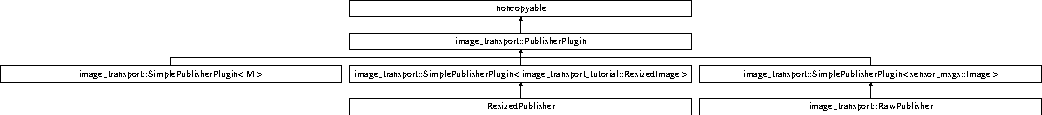
\includegraphics[height=1.545894cm]{classimage__transport_1_1_publisher_plugin}
\end{center}
\end{figure}
\subsection*{Public Member Functions}
\begin{DoxyCompactItemize}
\item 
\hypertarget{classimage__transport_1_1_publisher_plugin_abe0cd36dc3c170adb6aec8bc6d81d52e}{virtual std\-::string \hyperlink{classimage__transport_1_1_publisher_plugin_abe0cd36dc3c170adb6aec8bc6d81d52e}{get\-Transport\-Name} () const =0}\label{classimage__transport_1_1_publisher_plugin_abe0cd36dc3c170adb6aec8bc6d81d52e}

\begin{DoxyCompactList}\small\item\em Get a string identifier for the transport provided by this plugin. \end{DoxyCompactList}\item 
\hypertarget{classimage__transport_1_1_publisher_plugin_aa79894b876115d4993fad934e200ad48}{void \hyperlink{classimage__transport_1_1_publisher_plugin_aa79894b876115d4993fad934e200ad48}{advertise} (ros\-::\-Node\-Handle \&nh, const std\-::string \&base\-\_\-topic, uint32\-\_\-t queue\-\_\-size, bool latch=true)}\label{classimage__transport_1_1_publisher_plugin_aa79894b876115d4993fad934e200ad48}

\begin{DoxyCompactList}\small\item\em Advertise a topic, simple version. \end{DoxyCompactList}\item 
\hypertarget{classimage__transport_1_1_publisher_plugin_aa05d1be5ed987a1074b480ef9d6d93ea}{void \hyperlink{classimage__transport_1_1_publisher_plugin_aa05d1be5ed987a1074b480ef9d6d93ea}{advertise} (ros\-::\-Node\-Handle \&nh, const std\-::string \&base\-\_\-topic, uint32\-\_\-t queue\-\_\-size, const Subscriber\-Status\-Callback \&connect\-\_\-cb, const Subscriber\-Status\-Callback \&disconnect\-\_\-cb=Subscriber\-Status\-Callback(), const ros\-::\-Void\-Ptr \&tracked\-\_\-object=ros\-::\-Void\-Ptr(), bool latch=true)}\label{classimage__transport_1_1_publisher_plugin_aa05d1be5ed987a1074b480ef9d6d93ea}

\begin{DoxyCompactList}\small\item\em Advertise a topic with subscriber status callbacks. \end{DoxyCompactList}\item 
\hypertarget{classimage__transport_1_1_publisher_plugin_a10afba12d403ba21536610fce596c856}{virtual uint32\-\_\-t \hyperlink{classimage__transport_1_1_publisher_plugin_a10afba12d403ba21536610fce596c856}{get\-Num\-Subscribers} () const =0}\label{classimage__transport_1_1_publisher_plugin_a10afba12d403ba21536610fce596c856}

\begin{DoxyCompactList}\small\item\em Returns the number of subscribers that are currently connected to this \hyperlink{classimage__transport_1_1_publisher_plugin}{Publisher\-Plugin}. \end{DoxyCompactList}\item 
\hypertarget{classimage__transport_1_1_publisher_plugin_ac00807561a7e3406472273b85f1036e8}{virtual std\-::string \hyperlink{classimage__transport_1_1_publisher_plugin_ac00807561a7e3406472273b85f1036e8}{get\-Topic} () const =0}\label{classimage__transport_1_1_publisher_plugin_ac00807561a7e3406472273b85f1036e8}

\begin{DoxyCompactList}\small\item\em Returns the communication topic that this \hyperlink{classimage__transport_1_1_publisher_plugin}{Publisher\-Plugin} will publish on. \end{DoxyCompactList}\item 
\hypertarget{classimage__transport_1_1_publisher_plugin_a9c17e85717c5478011c944998d9f1bff}{virtual void \hyperlink{classimage__transport_1_1_publisher_plugin_a9c17e85717c5478011c944998d9f1bff}{publish} (const sensor\-\_\-msgs\-::\-Image \&message) const =0}\label{classimage__transport_1_1_publisher_plugin_a9c17e85717c5478011c944998d9f1bff}

\begin{DoxyCompactList}\small\item\em Publish an image using the transport associated with this \hyperlink{classimage__transport_1_1_publisher_plugin}{Publisher\-Plugin}. \end{DoxyCompactList}\item 
\hypertarget{classimage__transport_1_1_publisher_plugin_a5ec0ad17a8f0ef7b966089c3b8f6ee60}{virtual void \hyperlink{classimage__transport_1_1_publisher_plugin_a5ec0ad17a8f0ef7b966089c3b8f6ee60}{publish} (const sensor\-\_\-msgs\-::\-Image\-Const\-Ptr \&message) const }\label{classimage__transport_1_1_publisher_plugin_a5ec0ad17a8f0ef7b966089c3b8f6ee60}

\begin{DoxyCompactList}\small\item\em Publish an image using the transport associated with this \hyperlink{classimage__transport_1_1_publisher_plugin}{Publisher\-Plugin}. \end{DoxyCompactList}\item 
virtual void \hyperlink{classimage__transport_1_1_publisher_plugin_add246a58e2cc57ceba3c957f52a95a6d}{publish} (const sensor\-\_\-msgs\-::\-Image \&message, const uint8\-\_\-t $\ast$data) const 
\begin{DoxyCompactList}\small\item\em Publish an image using the transport associated with this \hyperlink{classimage__transport_1_1_publisher_plugin}{Publisher\-Plugin}. This version of the function can be used to optimize cases where you don't want to fill a R\-O\-S message first to avoid useless copies. \end{DoxyCompactList}\item 
\hypertarget{classimage__transport_1_1_publisher_plugin_aebf86857a6453919807061565f8837d2}{virtual void \hyperlink{classimage__transport_1_1_publisher_plugin_aebf86857a6453919807061565f8837d2}{shutdown} ()=0}\label{classimage__transport_1_1_publisher_plugin_aebf86857a6453919807061565f8837d2}

\begin{DoxyCompactList}\small\item\em Shutdown any advertisements associated with this \hyperlink{classimage__transport_1_1_publisher_plugin}{Publisher\-Plugin}. \end{DoxyCompactList}\end{DoxyCompactItemize}
\subsection*{Static Public Member Functions}
\begin{DoxyCompactItemize}
\item 
\hypertarget{classimage__transport_1_1_publisher_plugin_ac509e7c5ce1a6ce07870968eb1e0a0e3}{static std\-::string \hyperlink{classimage__transport_1_1_publisher_plugin_ac509e7c5ce1a6ce07870968eb1e0a0e3}{get\-Lookup\-Name} (const std\-::string \&transport\-\_\-name)}\label{classimage__transport_1_1_publisher_plugin_ac509e7c5ce1a6ce07870968eb1e0a0e3}

\begin{DoxyCompactList}\small\item\em Return the lookup name of the \hyperlink{classimage__transport_1_1_publisher_plugin}{Publisher\-Plugin} associated with a specific transport identifier. \end{DoxyCompactList}\end{DoxyCompactItemize}
\subsection*{Protected Member Functions}
\begin{DoxyCompactItemize}
\item 
\hypertarget{classimage__transport_1_1_publisher_plugin_ab6452043d8f51ed52638abf470aa4884}{virtual void \hyperlink{classimage__transport_1_1_publisher_plugin_ab6452043d8f51ed52638abf470aa4884}{advertise\-Impl} (ros\-::\-Node\-Handle \&nh, const std\-::string \&base\-\_\-topic, uint32\-\_\-t queue\-\_\-size, const Subscriber\-Status\-Callback \&connect\-\_\-cb, const Subscriber\-Status\-Callback \&disconnect\-\_\-cb, const ros\-::\-Void\-Ptr \&tracked\-\_\-object, bool latch)=0}\label{classimage__transport_1_1_publisher_plugin_ab6452043d8f51ed52638abf470aa4884}

\begin{DoxyCompactList}\small\item\em Advertise a topic. Must be implemented by the subclass. \end{DoxyCompactList}\end{DoxyCompactItemize}


\subsection{Detailed Description}
Base class for plugins to \hyperlink{classimage__transport_1_1_publisher}{Publisher}. 

Definition at line 47 of file publisher\-\_\-plugin.\-h.



\subsection{Member Function Documentation}
\hypertarget{classimage__transport_1_1_publisher_plugin_add246a58e2cc57ceba3c957f52a95a6d}{\index{image\-\_\-transport\-::\-Publisher\-Plugin@{image\-\_\-transport\-::\-Publisher\-Plugin}!publish@{publish}}
\index{publish@{publish}!image_transport::PublisherPlugin@{image\-\_\-transport\-::\-Publisher\-Plugin}}
\subsubsection[{publish}]{\setlength{\rightskip}{0pt plus 5cm}virtual void image\-\_\-transport\-::\-Publisher\-Plugin\-::publish (
\begin{DoxyParamCaption}
\item[{const sensor\-\_\-msgs\-::\-Image \&}]{message, }
\item[{const uint8\-\_\-t $\ast$}]{data}
\end{DoxyParamCaption}
) const\hspace{0.3cm}{\ttfamily [inline]}, {\ttfamily [virtual]}}}\label{classimage__transport_1_1_publisher_plugin_add246a58e2cc57ceba3c957f52a95a6d}


Publish an image using the transport associated with this \hyperlink{classimage__transport_1_1_publisher_plugin}{Publisher\-Plugin}. This version of the function can be used to optimize cases where you don't want to fill a R\-O\-S message first to avoid useless copies. 


\begin{DoxyParams}{Parameters}
{\em message} & an image message to use information from (but not data) \\
\hline
{\em data} & a pointer to the image data to use to fill the Image message \\
\hline
\end{DoxyParams}


Reimplemented in \hyperlink{classimage__transport_1_1_raw_publisher_a62ee9d7dab3a361ad92c70a4df5d6416}{image\-\_\-transport\-::\-Raw\-Publisher}.



Definition at line 110 of file publisher\-\_\-plugin.\-h.



The documentation for this class was generated from the following file\-:\begin{DoxyCompactItemize}
\item 
/home/travis/catkin\-\_\-ws/src/image\-\_\-common/image\-\_\-transport/include/image\-\_\-transport/publisher\-\_\-plugin.\-h\end{DoxyCompactItemize}

\hypertarget{classmsckf_1_1_quaternion}{\section{msckf.\-Quaternion Class Reference}
\label{classmsckf_1_1_quaternion}\index{msckf.\-Quaternion@{msckf.\-Quaternion}}
}
\subsection*{Static Public Member Functions}
\begin{DoxyCompactItemize}
\item 
\hypertarget{classmsckf_1_1_quaternion_a0bd71eee1eb3c21c88e95dd7dad39b2b}{def {\bfseries to\-\_\-rotation\-\_\-matrix}}\label{classmsckf_1_1_quaternion_a0bd71eee1eb3c21c88e95dd7dad39b2b}

\item 
\hypertarget{classmsckf_1_1_quaternion_a1ad344e0e8b25fcedcea28e57dd1194b}{def {\bfseries to\-\_\-euler\-\_\-angles}}\label{classmsckf_1_1_quaternion_a1ad344e0e8b25fcedcea28e57dd1194b}

\item 
\hypertarget{classmsckf_1_1_quaternion_af96060fbd037864de9e4386cf32557f9}{def {\bfseries vector\-\_\-to\-\_\-quaternion\-\_\-form}}\label{classmsckf_1_1_quaternion_af96060fbd037864de9e4386cf32557f9}

\item 
\hypertarget{classmsckf_1_1_quaternion_a0c8379745cc348059060aed3a8abf67c}{def {\bfseries vector\-\_\-from\-\_\-quaternion\-\_\-form}}\label{classmsckf_1_1_quaternion_a0c8379745cc348059060aed3a8abf67c}

\item 
\hypertarget{classmsckf_1_1_quaternion_aaaa45c31c39141a8fb00c13dfda9635d}{def {\bfseries cross\-\_\-matrix}}\label{classmsckf_1_1_quaternion_aaaa45c31c39141a8fb00c13dfda9635d}

\item 
\hypertarget{classmsckf_1_1_quaternion_a492071a17aa06a82ab0a30abdc6211bf}{def {\bfseries big\-\_\-omega\-\_\-matrix}}\label{classmsckf_1_1_quaternion_a492071a17aa06a82ab0a30abdc6211bf}

\end{DoxyCompactItemize}


\subsection{Detailed Description}


Definition at line 44 of file msckf.\-py.



The documentation for this class was generated from the following file\-:\begin{DoxyCompactItemize}
\item 
/home/travis/build/tomas789/tonav/prototype/msckf.\-py\end{DoxyCompactItemize}

\hypertarget{classimage__transport_1_1_raw_publisher}{\section{image\-\_\-transport\-:\-:Raw\-Publisher Class Reference}
\label{classimage__transport_1_1_raw_publisher}\index{image\-\_\-transport\-::\-Raw\-Publisher@{image\-\_\-transport\-::\-Raw\-Publisher}}
}


The default \hyperlink{classimage__transport_1_1_publisher_plugin}{Publisher\-Plugin}.  




{\ttfamily \#include $<$raw\-\_\-publisher.\-h$>$}

Inheritance diagram for image\-\_\-transport\-:\-:Raw\-Publisher\-:\begin{figure}[H]
\begin{center}
\leavevmode
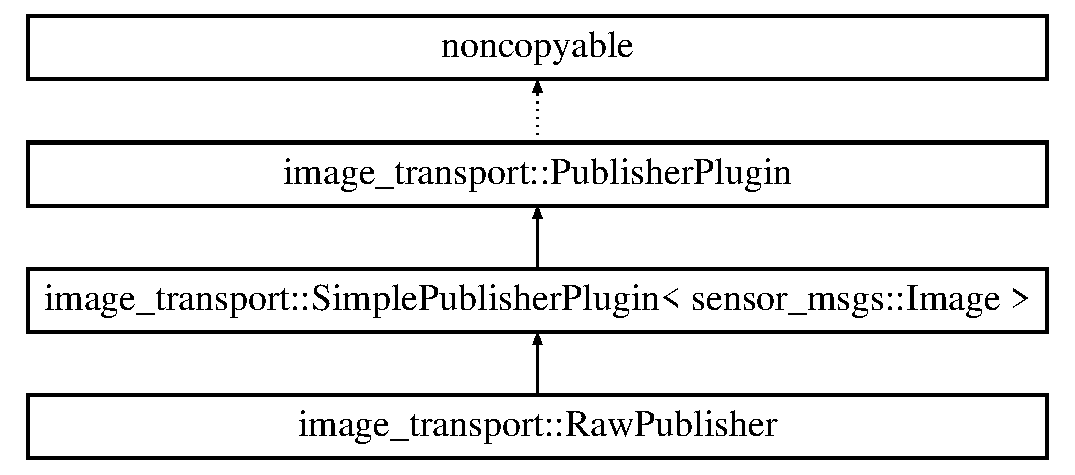
\includegraphics[height=4.000000cm]{classimage__transport_1_1_raw_publisher}
\end{center}
\end{figure}
\subsection*{Public Member Functions}
\begin{DoxyCompactItemize}
\item 
\hypertarget{classimage__transport_1_1_raw_publisher_adbb149bca794283f80db9df4c32f34dc}{virtual std\-::string \hyperlink{classimage__transport_1_1_raw_publisher_adbb149bca794283f80db9df4c32f34dc}{get\-Transport\-Name} () const }\label{classimage__transport_1_1_raw_publisher_adbb149bca794283f80db9df4c32f34dc}

\begin{DoxyCompactList}\small\item\em Get a string identifier for the transport provided by this plugin. \end{DoxyCompactList}\item 
\hypertarget{classimage__transport_1_1_raw_publisher_a567f1bc6ddaf5fc191fda71d4e5b4d22}{virtual void \hyperlink{classimage__transport_1_1_raw_publisher_a567f1bc6ddaf5fc191fda71d4e5b4d22}{publish} (const sensor\-\_\-msgs\-::\-Image\-Const\-Ptr \&message) const }\label{classimage__transport_1_1_raw_publisher_a567f1bc6ddaf5fc191fda71d4e5b4d22}

\begin{DoxyCompactList}\small\item\em Publish an image using the transport associated with this \hyperlink{classimage__transport_1_1_publisher_plugin}{Publisher\-Plugin}. \end{DoxyCompactList}\item 
virtual void \hyperlink{classimage__transport_1_1_raw_publisher_a62ee9d7dab3a361ad92c70a4df5d6416}{publish} (const sensor\-\_\-msgs\-::\-Image \&message, const uint8\-\_\-t $\ast$data) const 
\begin{DoxyCompactList}\small\item\em Publish an image using the transport associated with this \hyperlink{classimage__transport_1_1_publisher_plugin}{Publisher\-Plugin}. This version of the function can be used to optimize cases where you don't want to fill a R\-O\-S message first to avoid useless copies. \end{DoxyCompactList}\end{DoxyCompactItemize}
\subsection*{Protected Member Functions}
\begin{DoxyCompactItemize}
\item 
virtual void \hyperlink{classimage__transport_1_1_raw_publisher_a5d82f75d47a79f1df0be82165398e8fa}{publish} (const sensor\-\_\-msgs\-::\-Image \&message, const \hyperlink{classimage__transport_1_1_simple_publisher_plugin_a01bd11cb3ee6b7ce6715a3b57feadf93}{Publish\-Fn} \&publish\-\_\-fn) const 
\begin{DoxyCompactList}\small\item\em Publish an image using the specified publish function. Must be implemented by the subclass. \end{DoxyCompactList}\item 
virtual std\-::string \hyperlink{classimage__transport_1_1_raw_publisher_a18a9e588fde64cffdf43a3cebba7b471}{get\-Topic\-To\-Advertise} (const std\-::string \&base\-\_\-topic) const 
\begin{DoxyCompactList}\small\item\em Return the communication topic name for a given base topic. \end{DoxyCompactList}\end{DoxyCompactItemize}
\subsection*{Additional Inherited Members}


\subsection{Detailed Description}
The default \hyperlink{classimage__transport_1_1_publisher_plugin}{Publisher\-Plugin}. 

\hyperlink{classimage__transport_1_1_raw_publisher}{Raw\-Publisher} is a simple wrapper for ros\-::\-Publisher, publishing unaltered Image messages on the base topic. 

Definition at line 48 of file raw\-\_\-publisher.\-h.



\subsection{Member Function Documentation}
\hypertarget{classimage__transport_1_1_raw_publisher_a18a9e588fde64cffdf43a3cebba7b471}{\index{image\-\_\-transport\-::\-Raw\-Publisher@{image\-\_\-transport\-::\-Raw\-Publisher}!get\-Topic\-To\-Advertise@{get\-Topic\-To\-Advertise}}
\index{get\-Topic\-To\-Advertise@{get\-Topic\-To\-Advertise}!image_transport::RawPublisher@{image\-\_\-transport\-::\-Raw\-Publisher}}
\subsubsection[{get\-Topic\-To\-Advertise}]{\setlength{\rightskip}{0pt plus 5cm}virtual std\-::string image\-\_\-transport\-::\-Raw\-Publisher\-::get\-Topic\-To\-Advertise (
\begin{DoxyParamCaption}
\item[{const std\-::string \&}]{base\-\_\-topic}
\end{DoxyParamCaption}
) const\hspace{0.3cm}{\ttfamily [inline]}, {\ttfamily [protected]}, {\ttfamily [virtual]}}}\label{classimage__transport_1_1_raw_publisher_a18a9e588fde64cffdf43a3cebba7b471}


Return the communication topic name for a given base topic. 

Defaults to $<$base topic$>$/$<$transport name$>$. 

Reimplemented from \hyperlink{classimage__transport_1_1_simple_publisher_plugin_a46df2b43de62c169d28ac510010d032f}{image\-\_\-transport\-::\-Simple\-Publisher\-Plugin$<$ sensor\-\_\-msgs\-::\-Image $>$}.



Definition at line 74 of file raw\-\_\-publisher.\-h.

\hypertarget{classimage__transport_1_1_raw_publisher_a62ee9d7dab3a361ad92c70a4df5d6416}{\index{image\-\_\-transport\-::\-Raw\-Publisher@{image\-\_\-transport\-::\-Raw\-Publisher}!publish@{publish}}
\index{publish@{publish}!image_transport::RawPublisher@{image\-\_\-transport\-::\-Raw\-Publisher}}
\subsubsection[{publish}]{\setlength{\rightskip}{0pt plus 5cm}virtual void image\-\_\-transport\-::\-Raw\-Publisher\-::publish (
\begin{DoxyParamCaption}
\item[{const sensor\-\_\-msgs\-::\-Image \&}]{message, }
\item[{const uint8\-\_\-t $\ast$}]{data}
\end{DoxyParamCaption}
) const\hspace{0.3cm}{\ttfamily [virtual]}}}\label{classimage__transport_1_1_raw_publisher_a62ee9d7dab3a361ad92c70a4df5d6416}


Publish an image using the transport associated with this \hyperlink{classimage__transport_1_1_publisher_plugin}{Publisher\-Plugin}. This version of the function can be used to optimize cases where you don't want to fill a R\-O\-S message first to avoid useless copies. 


\begin{DoxyParams}{Parameters}
{\em message} & an image message to use information from (but not data) \\
\hline
{\em data} & a pointer to the image data to use to fill the Image message \\
\hline
\end{DoxyParams}


Reimplemented from \hyperlink{classimage__transport_1_1_publisher_plugin_add246a58e2cc57ceba3c957f52a95a6d}{image\-\_\-transport\-::\-Publisher\-Plugin}.

\hypertarget{classimage__transport_1_1_raw_publisher_a5d82f75d47a79f1df0be82165398e8fa}{\index{image\-\_\-transport\-::\-Raw\-Publisher@{image\-\_\-transport\-::\-Raw\-Publisher}!publish@{publish}}
\index{publish@{publish}!image_transport::RawPublisher@{image\-\_\-transport\-::\-Raw\-Publisher}}
\subsubsection[{publish}]{\setlength{\rightskip}{0pt plus 5cm}virtual void image\-\_\-transport\-::\-Raw\-Publisher\-::publish (
\begin{DoxyParamCaption}
\item[{const sensor\-\_\-msgs\-::\-Image \&}]{message, }
\item[{const {\bf Publish\-Fn} \&}]{publish\-\_\-fn}
\end{DoxyParamCaption}
) const\hspace{0.3cm}{\ttfamily [inline]}, {\ttfamily [protected]}, {\ttfamily [virtual]}}}\label{classimage__transport_1_1_raw_publisher_a5d82f75d47a79f1df0be82165398e8fa}


Publish an image using the specified publish function. Must be implemented by the subclass. 

The Publish\-Fn publishes the transport-\/specific message type. This indirection allows \hyperlink{classimage__transport_1_1_simple_subscriber_plugin}{Simple\-Subscriber\-Plugin} to use this function for both normal broadcast publishing and single subscriber publishing (in subscription callbacks). 

Implements \hyperlink{classimage__transport_1_1_simple_publisher_plugin_a193470dd32092d13e2284052d4fa359a}{image\-\_\-transport\-::\-Simple\-Publisher\-Plugin$<$ sensor\-\_\-msgs\-::\-Image $>$}.



Definition at line 69 of file raw\-\_\-publisher.\-h.



The documentation for this class was generated from the following file\-:\begin{DoxyCompactItemize}
\item 
/home/travis/catkin\-\_\-ws/src/image\-\_\-common/image\-\_\-transport/include/image\-\_\-transport/raw\-\_\-publisher.\-h\end{DoxyCompactItemize}

\hypertarget{classimage__transport_1_1_raw_subscriber}{\section{image\-\_\-transport\-:\-:Raw\-Subscriber Class Reference}
\label{classimage__transport_1_1_raw_subscriber}\index{image\-\_\-transport\-::\-Raw\-Subscriber@{image\-\_\-transport\-::\-Raw\-Subscriber}}
}


The default \hyperlink{classimage__transport_1_1_subscriber_plugin}{Subscriber\-Plugin}.  




{\ttfamily \#include $<$raw\-\_\-subscriber.\-h$>$}

Inheritance diagram for image\-\_\-transport\-:\-:Raw\-Subscriber\-:\begin{figure}[H]
\begin{center}
\leavevmode
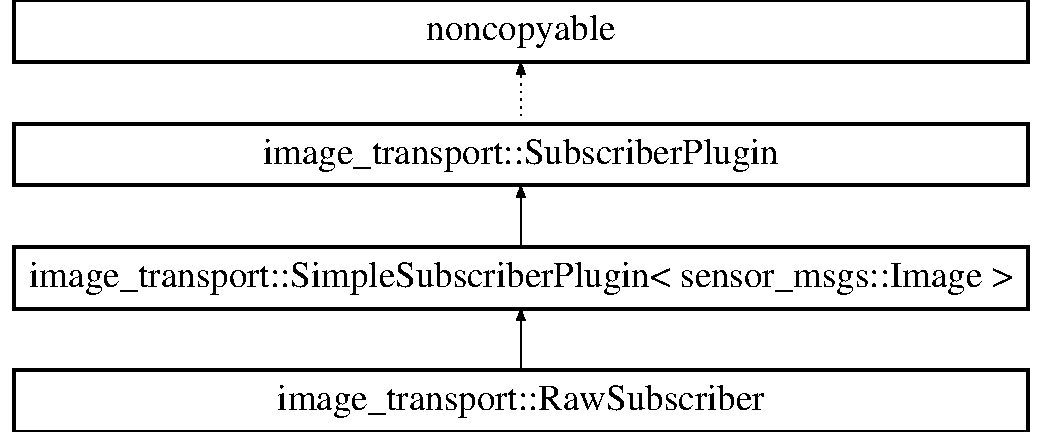
\includegraphics[height=4.000000cm]{classimage__transport_1_1_raw_subscriber}
\end{center}
\end{figure}
\subsection*{Public Member Functions}
\begin{DoxyCompactItemize}
\item 
\hypertarget{classimage__transport_1_1_raw_subscriber_a9c570fff1410a5b3f0fa40bc9705d135}{virtual std\-::string \hyperlink{classimage__transport_1_1_raw_subscriber_a9c570fff1410a5b3f0fa40bc9705d135}{get\-Transport\-Name} () const }\label{classimage__transport_1_1_raw_subscriber_a9c570fff1410a5b3f0fa40bc9705d135}

\begin{DoxyCompactList}\small\item\em Get a string identifier for the transport provided by this plugin. \end{DoxyCompactList}\end{DoxyCompactItemize}
\subsection*{Protected Member Functions}
\begin{DoxyCompactItemize}
\item 
\hypertarget{classimage__transport_1_1_raw_subscriber_a66df34f75b6dbab383de759bb0fa60b2}{virtual void {\bfseries internal\-Callback} (const sensor\-\_\-msgs\-::\-Image\-Const\-Ptr \&message, const Callback \&user\-\_\-cb)}\label{classimage__transport_1_1_raw_subscriber_a66df34f75b6dbab383de759bb0fa60b2}

\item 
virtual std\-::string \hyperlink{classimage__transport_1_1_raw_subscriber_a6da2134193b87fb71afda535a618cc7c}{get\-Topic\-To\-Subscribe} (const std\-::string \&base\-\_\-topic) const 
\begin{DoxyCompactList}\small\item\em Return the communication topic name for a given base topic. \end{DoxyCompactList}\end{DoxyCompactItemize}
\subsection*{Additional Inherited Members}


\subsection{Detailed Description}
The default \hyperlink{classimage__transport_1_1_subscriber_plugin}{Subscriber\-Plugin}. 

\hyperlink{classimage__transport_1_1_raw_subscriber}{Raw\-Subscriber} is a simple wrapper for ros\-::\-Subscriber which listens for Image messages and passes them through to the callback. 

Definition at line 48 of file raw\-\_\-subscriber.\-h.



\subsection{Member Function Documentation}
\hypertarget{classimage__transport_1_1_raw_subscriber_a6da2134193b87fb71afda535a618cc7c}{\index{image\-\_\-transport\-::\-Raw\-Subscriber@{image\-\_\-transport\-::\-Raw\-Subscriber}!get\-Topic\-To\-Subscribe@{get\-Topic\-To\-Subscribe}}
\index{get\-Topic\-To\-Subscribe@{get\-Topic\-To\-Subscribe}!image_transport::RawSubscriber@{image\-\_\-transport\-::\-Raw\-Subscriber}}
\subsubsection[{get\-Topic\-To\-Subscribe}]{\setlength{\rightskip}{0pt plus 5cm}virtual std\-::string image\-\_\-transport\-::\-Raw\-Subscriber\-::get\-Topic\-To\-Subscribe (
\begin{DoxyParamCaption}
\item[{const std\-::string \&}]{base\-\_\-topic}
\end{DoxyParamCaption}
) const\hspace{0.3cm}{\ttfamily [inline]}, {\ttfamily [protected]}, {\ttfamily [virtual]}}}\label{classimage__transport_1_1_raw_subscriber_a6da2134193b87fb71afda535a618cc7c}


Return the communication topic name for a given base topic. 

Defaults to $<$base topic$>$/$<$transport name$>$. 

Reimplemented from \hyperlink{classimage__transport_1_1_simple_subscriber_plugin_a02016ab17568754d5319ae6fd949e268}{image\-\_\-transport\-::\-Simple\-Subscriber\-Plugin$<$ sensor\-\_\-msgs\-::\-Image $>$}.



Definition at line 64 of file raw\-\_\-subscriber.\-h.



The documentation for this class was generated from the following file\-:\begin{DoxyCompactItemize}
\item 
/home/travis/catkin\-\_\-ws/src/image\-\_\-common/image\-\_\-transport/include/image\-\_\-transport/raw\-\_\-subscriber.\-h\end{DoxyCompactItemize}

\hypertarget{class_resized_publisher}{\section{Resized\-Publisher Class Reference}
\label{class_resized_publisher}\index{Resized\-Publisher@{Resized\-Publisher}}
}
Inheritance diagram for Resized\-Publisher\-:\begin{figure}[H]
\begin{center}
\leavevmode
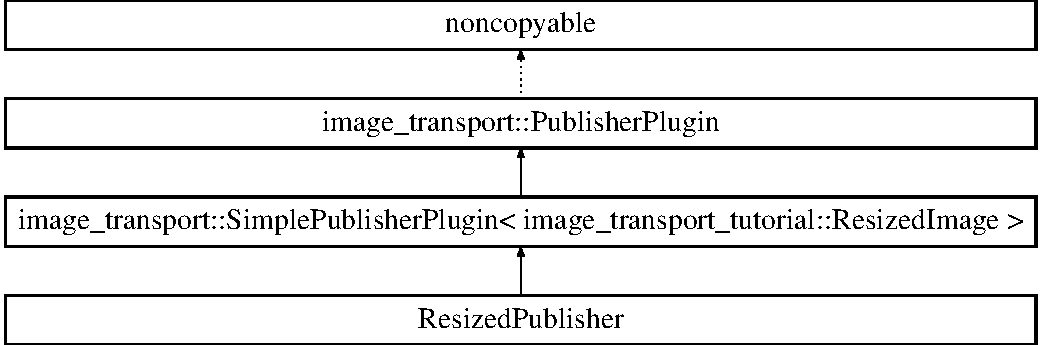
\includegraphics[height=4.000000cm]{class_resized_publisher}
\end{center}
\end{figure}
\subsection*{Public Member Functions}
\begin{DoxyCompactItemize}
\item 
\hypertarget{class_resized_publisher_a2282c668269cc359be3f1767fa31c1cc}{virtual std\-::string \hyperlink{class_resized_publisher_a2282c668269cc359be3f1767fa31c1cc}{get\-Transport\-Name} () const }\label{class_resized_publisher_a2282c668269cc359be3f1767fa31c1cc}

\begin{DoxyCompactList}\small\item\em Get a string identifier for the transport provided by this plugin. \end{DoxyCompactList}\end{DoxyCompactItemize}
\subsection*{Protected Member Functions}
\begin{DoxyCompactItemize}
\item 
virtual void \hyperlink{class_resized_publisher_af0121f511226071f7cb96fb3e50879a6}{publish} (const sensor\-\_\-msgs\-::\-Image \&message, const \hyperlink{classimage__transport_1_1_simple_publisher_plugin_a01bd11cb3ee6b7ce6715a3b57feadf93}{Publish\-Fn} \&publish\-\_\-fn) const 
\begin{DoxyCompactList}\small\item\em Publish an image using the specified publish function. Must be implemented by the subclass. \end{DoxyCompactList}\end{DoxyCompactItemize}
\subsection*{Additional Inherited Members}


\subsection{Detailed Description}


Definition at line 4 of file resized\-\_\-publisher.\-h.



\subsection{Member Function Documentation}
\hypertarget{class_resized_publisher_af0121f511226071f7cb96fb3e50879a6}{\index{Resized\-Publisher@{Resized\-Publisher}!publish@{publish}}
\index{publish@{publish}!ResizedPublisher@{Resized\-Publisher}}
\subsubsection[{publish}]{\setlength{\rightskip}{0pt plus 5cm}void Resized\-Publisher\-::publish (
\begin{DoxyParamCaption}
\item[{const sensor\-\_\-msgs\-::\-Image \&}]{message, }
\item[{const {\bf Publish\-Fn} \&}]{publish\-\_\-fn}
\end{DoxyParamCaption}
) const\hspace{0.3cm}{\ttfamily [protected]}, {\ttfamily [virtual]}}}\label{class_resized_publisher_af0121f511226071f7cb96fb3e50879a6}


Publish an image using the specified publish function. Must be implemented by the subclass. 

The Publish\-Fn publishes the transport-\/specific message type. This indirection allows Simple\-Subscriber\-Plugin to use this function for both normal broadcast publishing and single subscriber publishing (in subscription callbacks). 

Implements \hyperlink{classimage__transport_1_1_simple_publisher_plugin_a193470dd32092d13e2284052d4fa359a}{image\-\_\-transport\-::\-Simple\-Publisher\-Plugin$<$ image\-\_\-transport\-\_\-tutorial\-::\-Resized\-Image $>$}.



Definition at line 5 of file resized\-\_\-publisher.\-cpp.



The documentation for this class was generated from the following files\-:\begin{DoxyCompactItemize}
\item 
/home/travis/catkin\-\_\-ws/src/image\-\_\-common/image\-\_\-transport/tutorial/include/image\-\_\-transport\-\_\-tutorial/resized\-\_\-publisher.\-h\item 
/home/travis/catkin\-\_\-ws/src/image\-\_\-common/image\-\_\-transport/tutorial/src/resized\-\_\-publisher.\-cpp\end{DoxyCompactItemize}

\hypertarget{class_resized_subscriber}{\section{Resized\-Subscriber Class Reference}
\label{class_resized_subscriber}\index{Resized\-Subscriber@{Resized\-Subscriber}}
}
Inheritance diagram for Resized\-Subscriber\-:\begin{figure}[H]
\begin{center}
\leavevmode
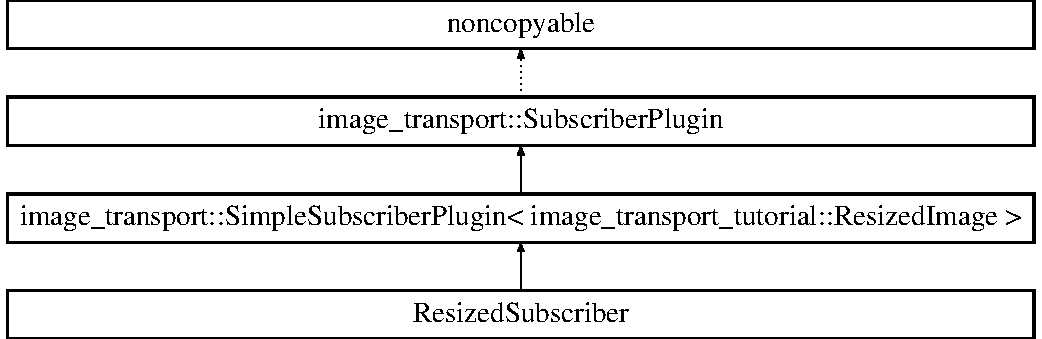
\includegraphics[height=4.000000cm]{class_resized_subscriber}
\end{center}
\end{figure}
\subsection*{Public Member Functions}
\begin{DoxyCompactItemize}
\item 
\hypertarget{class_resized_subscriber_abe804a1a73e5281d2e60f7ea6a82c9b8}{virtual std\-::string \hyperlink{class_resized_subscriber_abe804a1a73e5281d2e60f7ea6a82c9b8}{get\-Transport\-Name} () const }\label{class_resized_subscriber_abe804a1a73e5281d2e60f7ea6a82c9b8}

\begin{DoxyCompactList}\small\item\em Get a string identifier for the transport provided by this plugin. \end{DoxyCompactList}\end{DoxyCompactItemize}
\subsection*{Protected Member Functions}
\begin{DoxyCompactItemize}
\item 
virtual void \hyperlink{class_resized_subscriber_ad0a3debf9a2135bbbae6145cebb958e8}{internal\-Callback} (const typename image\-\_\-transport\-\_\-tutorial\-::\-Resized\-Image\-::\-Const\-Ptr \&message, const Callback \&user\-\_\-cb)
\begin{DoxyCompactList}\small\item\em Process a message. Must be implemented by the subclass. \end{DoxyCompactList}\end{DoxyCompactItemize}
\subsection*{Additional Inherited Members}


\subsection{Detailed Description}


Definition at line 4 of file resized\-\_\-subscriber.\-h.



\subsection{Member Function Documentation}
\hypertarget{class_resized_subscriber_ad0a3debf9a2135bbbae6145cebb958e8}{\index{Resized\-Subscriber@{Resized\-Subscriber}!internal\-Callback@{internal\-Callback}}
\index{internal\-Callback@{internal\-Callback}!ResizedSubscriber@{Resized\-Subscriber}}
\subsubsection[{internal\-Callback}]{\setlength{\rightskip}{0pt plus 5cm}void Resized\-Subscriber\-::internal\-Callback (
\begin{DoxyParamCaption}
\item[{const typename image\-\_\-transport\-\_\-tutorial\-::\-Resized\-Image\-::\-Const\-Ptr \&}]{message, }
\item[{const Callback \&}]{user\-\_\-cb}
\end{DoxyParamCaption}
)\hspace{0.3cm}{\ttfamily [protected]}, {\ttfamily [virtual]}}}\label{class_resized_subscriber_ad0a3debf9a2135bbbae6145cebb958e8}


Process a message. Must be implemented by the subclass. 


\begin{DoxyParams}{Parameters}
{\em message} & A message from the Publisher\-Plugin. \\
\hline
{\em user\-\_\-cb} & The user Image callback to invoke, if appropriate. \\
\hline
\end{DoxyParams}


Implements \hyperlink{classimage__transport_1_1_simple_subscriber_plugin_ae3fbeb43694289e50670d7050da82a1a}{image\-\_\-transport\-::\-Simple\-Subscriber\-Plugin$<$ image\-\_\-transport\-\_\-tutorial\-::\-Resized\-Image $>$}.



Definition at line 5 of file resized\-\_\-subscriber.\-cpp.



The documentation for this class was generated from the following files\-:\begin{DoxyCompactItemize}
\item 
/home/travis/catkin\-\_\-ws/src/image\-\_\-common/image\-\_\-transport/tutorial/include/image\-\_\-transport\-\_\-tutorial/resized\-\_\-subscriber.\-h\item 
/home/travis/catkin\-\_\-ws/src/image\-\_\-common/image\-\_\-transport/tutorial/src/resized\-\_\-subscriber.\-cpp\end{DoxyCompactItemize}

\hypertarget{classimage__transport_1_1_simple_publisher_plugin}{\section{image\-\_\-transport\-:\-:Simple\-Publisher\-Plugin$<$ M $>$ Class Template Reference}
\label{classimage__transport_1_1_simple_publisher_plugin}\index{image\-\_\-transport\-::\-Simple\-Publisher\-Plugin$<$ M $>$@{image\-\_\-transport\-::\-Simple\-Publisher\-Plugin$<$ M $>$}}
}


Base class to simplify implementing most plugins to \hyperlink{classimage__transport_1_1_publisher}{Publisher}.  




{\ttfamily \#include $<$simple\-\_\-publisher\-\_\-plugin.\-h$>$}

Inheritance diagram for image\-\_\-transport\-:\-:Simple\-Publisher\-Plugin$<$ M $>$\-:\begin{figure}[H]
\begin{center}
\leavevmode
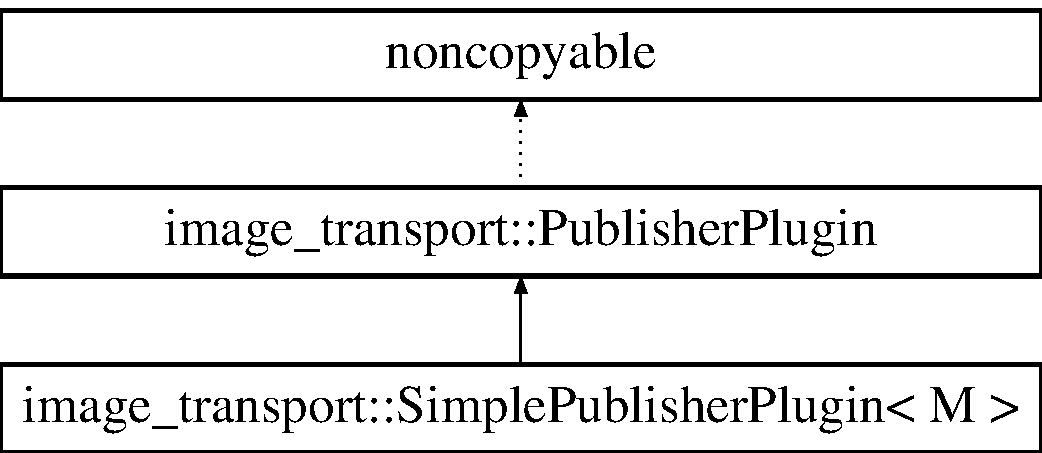
\includegraphics[height=3.000000cm]{classimage__transport_1_1_simple_publisher_plugin}
\end{center}
\end{figure}
\subsection*{Public Member Functions}
\begin{DoxyCompactItemize}
\item 
\hypertarget{classimage__transport_1_1_simple_publisher_plugin_a58697b43b16d32531b4f67a7c8709f20}{virtual uint32\-\_\-t \hyperlink{classimage__transport_1_1_simple_publisher_plugin_a58697b43b16d32531b4f67a7c8709f20}{get\-Num\-Subscribers} () const }\label{classimage__transport_1_1_simple_publisher_plugin_a58697b43b16d32531b4f67a7c8709f20}

\begin{DoxyCompactList}\small\item\em Returns the number of subscribers that are currently connected to this \hyperlink{classimage__transport_1_1_publisher_plugin}{Publisher\-Plugin}. \end{DoxyCompactList}\item 
\hypertarget{classimage__transport_1_1_simple_publisher_plugin_a24f9923dbde675f1693b1be252805918}{virtual std\-::string \hyperlink{classimage__transport_1_1_simple_publisher_plugin_a24f9923dbde675f1693b1be252805918}{get\-Topic} () const }\label{classimage__transport_1_1_simple_publisher_plugin_a24f9923dbde675f1693b1be252805918}

\begin{DoxyCompactList}\small\item\em Returns the communication topic that this \hyperlink{classimage__transport_1_1_publisher_plugin}{Publisher\-Plugin} will publish on. \end{DoxyCompactList}\item 
\hypertarget{classimage__transport_1_1_simple_publisher_plugin_a409f2078d4aa3466e843404b88cfe101}{virtual void \hyperlink{classimage__transport_1_1_simple_publisher_plugin_a409f2078d4aa3466e843404b88cfe101}{publish} (const sensor\-\_\-msgs\-::\-Image \&message) const }\label{classimage__transport_1_1_simple_publisher_plugin_a409f2078d4aa3466e843404b88cfe101}

\begin{DoxyCompactList}\small\item\em Publish an image using the transport associated with this \hyperlink{classimage__transport_1_1_publisher_plugin}{Publisher\-Plugin}. \end{DoxyCompactList}\item 
\hypertarget{classimage__transport_1_1_simple_publisher_plugin_a62e2d4cce1756530fbf6a323b1a00c59}{virtual void \hyperlink{classimage__transport_1_1_simple_publisher_plugin_a62e2d4cce1756530fbf6a323b1a00c59}{shutdown} ()}\label{classimage__transport_1_1_simple_publisher_plugin_a62e2d4cce1756530fbf6a323b1a00c59}

\begin{DoxyCompactList}\small\item\em Shutdown any advertisements associated with this \hyperlink{classimage__transport_1_1_publisher_plugin}{Publisher\-Plugin}. \end{DoxyCompactList}\end{DoxyCompactItemize}
\subsection*{Protected Types}
\begin{DoxyCompactItemize}
\item 
\hypertarget{classimage__transport_1_1_simple_publisher_plugin_a01bd11cb3ee6b7ce6715a3b57feadf93}{typedef boost\-::function$<$ void(const \\*
M \&)$>$ \hyperlink{classimage__transport_1_1_simple_publisher_plugin_a01bd11cb3ee6b7ce6715a3b57feadf93}{Publish\-Fn}}\label{classimage__transport_1_1_simple_publisher_plugin_a01bd11cb3ee6b7ce6715a3b57feadf93}

\begin{DoxyCompactList}\small\item\em Generic function for publishing the internal message type. \end{DoxyCompactList}\end{DoxyCompactItemize}
\subsection*{Protected Member Functions}
\begin{DoxyCompactItemize}
\item 
\hypertarget{classimage__transport_1_1_simple_publisher_plugin_af9ca774ef9d18a9cf745c92762c00d91}{virtual void \hyperlink{classimage__transport_1_1_simple_publisher_plugin_af9ca774ef9d18a9cf745c92762c00d91}{advertise\-Impl} (ros\-::\-Node\-Handle \&\hyperlink{classimage__transport_1_1_simple_publisher_plugin_a5f73a993e871242e51671f3cf82d4e1b}{nh}, const std\-::string \&base\-\_\-topic, uint32\-\_\-t queue\-\_\-size, const Subscriber\-Status\-Callback \&user\-\_\-connect\-\_\-cb, const Subscriber\-Status\-Callback \&user\-\_\-disconnect\-\_\-cb, const ros\-::\-Void\-Ptr \&tracked\-\_\-object, bool latch)}\label{classimage__transport_1_1_simple_publisher_plugin_af9ca774ef9d18a9cf745c92762c00d91}

\begin{DoxyCompactList}\small\item\em Advertise a topic. Must be implemented by the subclass. \end{DoxyCompactList}\item 
virtual void \hyperlink{classimage__transport_1_1_simple_publisher_plugin_a193470dd32092d13e2284052d4fa359a}{publish} (const sensor\-\_\-msgs\-::\-Image \&message, const \hyperlink{classimage__transport_1_1_simple_publisher_plugin_a01bd11cb3ee6b7ce6715a3b57feadf93}{Publish\-Fn} \&publish\-\_\-fn) const =0
\begin{DoxyCompactList}\small\item\em Publish an image using the specified publish function. Must be implemented by the subclass. \end{DoxyCompactList}\item 
virtual std\-::string \hyperlink{classimage__transport_1_1_simple_publisher_plugin_a46df2b43de62c169d28ac510010d032f}{get\-Topic\-To\-Advertise} (const std\-::string \&base\-\_\-topic) const 
\begin{DoxyCompactList}\small\item\em Return the communication topic name for a given base topic. \end{DoxyCompactList}\item 
virtual void \hyperlink{classimage__transport_1_1_simple_publisher_plugin_a4329bd192aa03ec8b44e52c6bbe91a11}{connect\-Callback} (const ros\-::\-Single\-Subscriber\-Publisher \&pub)
\begin{DoxyCompactList}\small\item\em Function called when a subscriber connects to the internal publisher. \end{DoxyCompactList}\item 
virtual void \hyperlink{classimage__transport_1_1_simple_publisher_plugin_ac02aac90a3a159c1450a298b63a37425}{disconnect\-Callback} (const ros\-::\-Single\-Subscriber\-Publisher \&pub)
\begin{DoxyCompactList}\small\item\em Function called when a subscriber disconnects from the internal publisher. \end{DoxyCompactList}\item 
\hypertarget{classimage__transport_1_1_simple_publisher_plugin_a5f73a993e871242e51671f3cf82d4e1b}{const ros\-::\-Node\-Handle \& \hyperlink{classimage__transport_1_1_simple_publisher_plugin_a5f73a993e871242e51671f3cf82d4e1b}{nh} () const }\label{classimage__transport_1_1_simple_publisher_plugin_a5f73a993e871242e51671f3cf82d4e1b}

\begin{DoxyCompactList}\small\item\em Returns the ros\-::\-Node\-Handle to be used for parameter lookup. \end{DoxyCompactList}\item 
const ros\-::\-Publisher \& \hyperlink{classimage__transport_1_1_simple_publisher_plugin_a11ad943c96711dc4a797a2b577ae9ea3}{get\-Publisher} () const 
\begin{DoxyCompactList}\small\item\em Returns the internal ros\-::\-Publisher. \end{DoxyCompactList}\end{DoxyCompactItemize}
\subsection*{Additional Inherited Members}


\subsection{Detailed Description}
\subsubsection*{template$<$class M$>$class image\-\_\-transport\-::\-Simple\-Publisher\-Plugin$<$ M $>$}

Base class to simplify implementing most plugins to \hyperlink{classimage__transport_1_1_publisher}{Publisher}. 

This base class vastly simplifies implementing a \hyperlink{classimage__transport_1_1_publisher_plugin}{Publisher\-Plugin} in the common case that all communication with the matching \hyperlink{classimage__transport_1_1_subscriber_plugin}{Subscriber\-Plugin} happens over a single R\-O\-S topic using a transport-\/specific message type. \hyperlink{classimage__transport_1_1_simple_publisher_plugin}{Simple\-Publisher\-Plugin} is templated on the transport-\/specific message type.

A subclass need implement only two methods\-:
\begin{DoxyItemize}
\item \hyperlink{classimage__transport_1_1_publisher_plugin_abe0cd36dc3c170adb6aec8bc6d81d52e}{get\-Transport\-Name()} from \hyperlink{classimage__transport_1_1_publisher_plugin}{Publisher\-Plugin}
\item \hyperlink{classimage__transport_1_1_simple_publisher_plugin_a409f2078d4aa3466e843404b88cfe101}{publish()} with an extra Publish\-Fn argument
\end{DoxyItemize}

For access to the parameter server and name remappings, use \hyperlink{classimage__transport_1_1_simple_publisher_plugin_a5f73a993e871242e51671f3cf82d4e1b}{nh()}.

\hyperlink{classimage__transport_1_1_simple_publisher_plugin_a46df2b43de62c169d28ac510010d032f}{get\-Topic\-To\-Advertise()} controls the name of the internal communication topic. It defaults to $<$base topic$>$/$<$transport name$>$. 

Definition at line 61 of file simple\-\_\-publisher\-\_\-plugin.\-h.



\subsection{Member Function Documentation}
\hypertarget{classimage__transport_1_1_simple_publisher_plugin_a4329bd192aa03ec8b44e52c6bbe91a11}{\index{image\-\_\-transport\-::\-Simple\-Publisher\-Plugin@{image\-\_\-transport\-::\-Simple\-Publisher\-Plugin}!connect\-Callback@{connect\-Callback}}
\index{connect\-Callback@{connect\-Callback}!image_transport::SimplePublisherPlugin@{image\-\_\-transport\-::\-Simple\-Publisher\-Plugin}}
\subsubsection[{connect\-Callback}]{\setlength{\rightskip}{0pt plus 5cm}template$<$class M$>$ virtual void {\bf image\-\_\-transport\-::\-Simple\-Publisher\-Plugin}$<$ M $>$\-::connect\-Callback (
\begin{DoxyParamCaption}
\item[{const ros\-::\-Single\-Subscriber\-Publisher \&}]{pub}
\end{DoxyParamCaption}
)\hspace{0.3cm}{\ttfamily [inline]}, {\ttfamily [protected]}, {\ttfamily [virtual]}}}\label{classimage__transport_1_1_simple_publisher_plugin_a4329bd192aa03ec8b44e52c6bbe91a11}


Function called when a subscriber connects to the internal publisher. 

Defaults to noop. 

Definition at line 136 of file simple\-\_\-publisher\-\_\-plugin.\-h.

\hypertarget{classimage__transport_1_1_simple_publisher_plugin_ac02aac90a3a159c1450a298b63a37425}{\index{image\-\_\-transport\-::\-Simple\-Publisher\-Plugin@{image\-\_\-transport\-::\-Simple\-Publisher\-Plugin}!disconnect\-Callback@{disconnect\-Callback}}
\index{disconnect\-Callback@{disconnect\-Callback}!image_transport::SimplePublisherPlugin@{image\-\_\-transport\-::\-Simple\-Publisher\-Plugin}}
\subsubsection[{disconnect\-Callback}]{\setlength{\rightskip}{0pt plus 5cm}template$<$class M$>$ virtual void {\bf image\-\_\-transport\-::\-Simple\-Publisher\-Plugin}$<$ M $>$\-::disconnect\-Callback (
\begin{DoxyParamCaption}
\item[{const ros\-::\-Single\-Subscriber\-Publisher \&}]{pub}
\end{DoxyParamCaption}
)\hspace{0.3cm}{\ttfamily [inline]}, {\ttfamily [protected]}, {\ttfamily [virtual]}}}\label{classimage__transport_1_1_simple_publisher_plugin_ac02aac90a3a159c1450a298b63a37425}


Function called when a subscriber disconnects from the internal publisher. 

Defaults to noop. 

Definition at line 143 of file simple\-\_\-publisher\-\_\-plugin.\-h.

\hypertarget{classimage__transport_1_1_simple_publisher_plugin_a11ad943c96711dc4a797a2b577ae9ea3}{\index{image\-\_\-transport\-::\-Simple\-Publisher\-Plugin@{image\-\_\-transport\-::\-Simple\-Publisher\-Plugin}!get\-Publisher@{get\-Publisher}}
\index{get\-Publisher@{get\-Publisher}!image_transport::SimplePublisherPlugin@{image\-\_\-transport\-::\-Simple\-Publisher\-Plugin}}
\subsubsection[{get\-Publisher}]{\setlength{\rightskip}{0pt plus 5cm}template$<$class M$>$ const ros\-::\-Publisher\& {\bf image\-\_\-transport\-::\-Simple\-Publisher\-Plugin}$<$ M $>$\-::get\-Publisher (
\begin{DoxyParamCaption}
{}
\end{DoxyParamCaption}
) const\hspace{0.3cm}{\ttfamily [inline]}, {\ttfamily [protected]}}}\label{classimage__transport_1_1_simple_publisher_plugin_a11ad943c96711dc4a797a2b577ae9ea3}


Returns the internal ros\-::\-Publisher. 

This really only exists so \hyperlink{classimage__transport_1_1_raw_publisher}{Raw\-Publisher} can implement no-\/copy intraprocess message passing easily. 

Definition at line 159 of file simple\-\_\-publisher\-\_\-plugin.\-h.

\hypertarget{classimage__transport_1_1_simple_publisher_plugin_a46df2b43de62c169d28ac510010d032f}{\index{image\-\_\-transport\-::\-Simple\-Publisher\-Plugin@{image\-\_\-transport\-::\-Simple\-Publisher\-Plugin}!get\-Topic\-To\-Advertise@{get\-Topic\-To\-Advertise}}
\index{get\-Topic\-To\-Advertise@{get\-Topic\-To\-Advertise}!image_transport::SimplePublisherPlugin@{image\-\_\-transport\-::\-Simple\-Publisher\-Plugin}}
\subsubsection[{get\-Topic\-To\-Advertise}]{\setlength{\rightskip}{0pt plus 5cm}template$<$class M$>$ virtual std\-::string {\bf image\-\_\-transport\-::\-Simple\-Publisher\-Plugin}$<$ M $>$\-::get\-Topic\-To\-Advertise (
\begin{DoxyParamCaption}
\item[{const std\-::string \&}]{base\-\_\-topic}
\end{DoxyParamCaption}
) const\hspace{0.3cm}{\ttfamily [inline]}, {\ttfamily [protected]}, {\ttfamily [virtual]}}}\label{classimage__transport_1_1_simple_publisher_plugin_a46df2b43de62c169d28ac510010d032f}


Return the communication topic name for a given base topic. 

Defaults to $<$base topic$>$/$<$transport name$>$. 

Reimplemented in \hyperlink{classimage__transport_1_1_raw_publisher_a18a9e588fde64cffdf43a3cebba7b471}{image\-\_\-transport\-::\-Raw\-Publisher}.



Definition at line 126 of file simple\-\_\-publisher\-\_\-plugin.\-h.

\hypertarget{classimage__transport_1_1_simple_publisher_plugin_a193470dd32092d13e2284052d4fa359a}{\index{image\-\_\-transport\-::\-Simple\-Publisher\-Plugin@{image\-\_\-transport\-::\-Simple\-Publisher\-Plugin}!publish@{publish}}
\index{publish@{publish}!image_transport::SimplePublisherPlugin@{image\-\_\-transport\-::\-Simple\-Publisher\-Plugin}}
\subsubsection[{publish}]{\setlength{\rightskip}{0pt plus 5cm}template$<$class M$>$ virtual void {\bf image\-\_\-transport\-::\-Simple\-Publisher\-Plugin}$<$ M $>$\-::publish (
\begin{DoxyParamCaption}
\item[{const sensor\-\_\-msgs\-::\-Image \&}]{message, }
\item[{const {\bf Publish\-Fn} \&}]{publish\-\_\-fn}
\end{DoxyParamCaption}
) const\hspace{0.3cm}{\ttfamily [protected]}, {\ttfamily [pure virtual]}}}\label{classimage__transport_1_1_simple_publisher_plugin_a193470dd32092d13e2284052d4fa359a}


Publish an image using the specified publish function. Must be implemented by the subclass. 

The Publish\-Fn publishes the transport-\/specific message type. This indirection allows \hyperlink{classimage__transport_1_1_simple_subscriber_plugin}{Simple\-Subscriber\-Plugin} to use this function for both normal broadcast publishing and single subscriber publishing (in subscription callbacks). 

Implemented in \hyperlink{classimage__transport_1_1_raw_publisher_a5d82f75d47a79f1df0be82165398e8fa}{image\-\_\-transport\-::\-Raw\-Publisher}, and \hyperlink{class_resized_publisher_af0121f511226071f7cb96fb3e50879a6}{Resized\-Publisher}.



The documentation for this class was generated from the following file\-:\begin{DoxyCompactItemize}
\item 
/home/travis/catkin\-\_\-ws/src/image\-\_\-common/image\-\_\-transport/include/image\-\_\-transport/simple\-\_\-publisher\-\_\-plugin.\-h\end{DoxyCompactItemize}

\hypertarget{classimage__transport_1_1_simple_subscriber_plugin}{\section{image\-\_\-transport\-:\-:Simple\-Subscriber\-Plugin$<$ M $>$ Class Template Reference}
\label{classimage__transport_1_1_simple_subscriber_plugin}\index{image\-\_\-transport\-::\-Simple\-Subscriber\-Plugin$<$ M $>$@{image\-\_\-transport\-::\-Simple\-Subscriber\-Plugin$<$ M $>$}}
}


Base class to simplify implementing most plugins to \hyperlink{classimage__transport_1_1_subscriber}{Subscriber}.  




{\ttfamily \#include $<$simple\-\_\-subscriber\-\_\-plugin.\-h$>$}

Inheritance diagram for image\-\_\-transport\-:\-:Simple\-Subscriber\-Plugin$<$ M $>$\-:\begin{figure}[H]
\begin{center}
\leavevmode
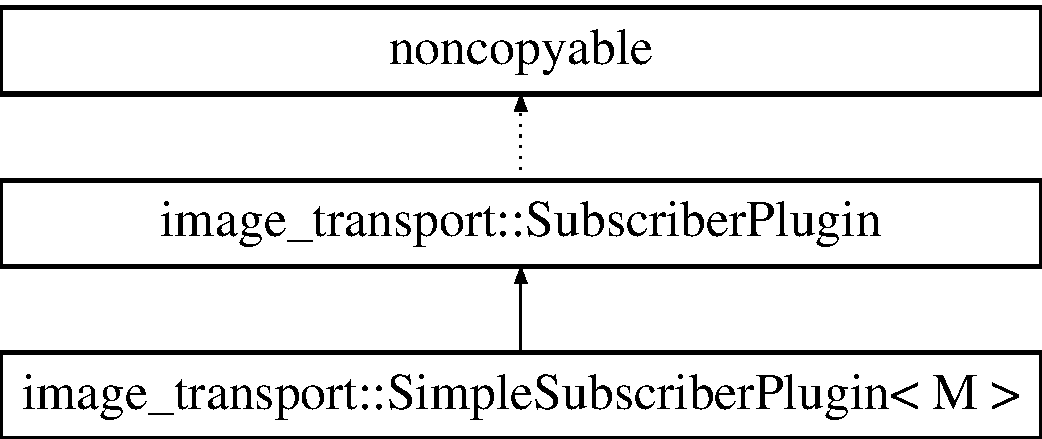
\includegraphics[height=3.000000cm]{classimage__transport_1_1_simple_subscriber_plugin}
\end{center}
\end{figure}
\subsection*{Public Member Functions}
\begin{DoxyCompactItemize}
\item 
\hypertarget{classimage__transport_1_1_simple_subscriber_plugin_ab6e2fa57778770429195a516b78dcb1a}{virtual std\-::string \hyperlink{classimage__transport_1_1_simple_subscriber_plugin_ab6e2fa57778770429195a516b78dcb1a}{get\-Topic} () const }\label{classimage__transport_1_1_simple_subscriber_plugin_ab6e2fa57778770429195a516b78dcb1a}

\begin{DoxyCompactList}\small\item\em Get the transport-\/specific communication topic. \end{DoxyCompactList}\item 
\hypertarget{classimage__transport_1_1_simple_subscriber_plugin_ae7115a373237561c9896fa93d74fe981}{virtual uint32\-\_\-t \hyperlink{classimage__transport_1_1_simple_subscriber_plugin_ae7115a373237561c9896fa93d74fe981}{get\-Num\-Publishers} () const }\label{classimage__transport_1_1_simple_subscriber_plugin_ae7115a373237561c9896fa93d74fe981}

\begin{DoxyCompactList}\small\item\em Returns the number of publishers this subscriber is connected to. \end{DoxyCompactList}\item 
\hypertarget{classimage__transport_1_1_simple_subscriber_plugin_a559eb7593e56faf92fbfba771e317455}{virtual void \hyperlink{classimage__transport_1_1_simple_subscriber_plugin_a559eb7593e56faf92fbfba771e317455}{shutdown} ()}\label{classimage__transport_1_1_simple_subscriber_plugin_a559eb7593e56faf92fbfba771e317455}

\begin{DoxyCompactList}\small\item\em Unsubscribe the callback associated with this \hyperlink{classimage__transport_1_1_subscriber_plugin}{Subscriber\-Plugin}. \end{DoxyCompactList}\end{DoxyCompactItemize}
\subsection*{Protected Member Functions}
\begin{DoxyCompactItemize}
\item 
virtual void \hyperlink{classimage__transport_1_1_simple_subscriber_plugin_ae3fbeb43694289e50670d7050da82a1a}{internal\-Callback} (const typename M\-::\-Const\-Ptr \&message, const Callback \&user\-\_\-cb)=0
\begin{DoxyCompactList}\small\item\em Process a message. Must be implemented by the subclass. \end{DoxyCompactList}\item 
virtual std\-::string \hyperlink{classimage__transport_1_1_simple_subscriber_plugin_a02016ab17568754d5319ae6fd949e268}{get\-Topic\-To\-Subscribe} (const std\-::string \&base\-\_\-topic) const 
\begin{DoxyCompactList}\small\item\em Return the communication topic name for a given base topic. \end{DoxyCompactList}\item 
\hypertarget{classimage__transport_1_1_simple_subscriber_plugin_adead418bf0be6f6511af9e6a03ab8322}{virtual void \hyperlink{classimage__transport_1_1_simple_subscriber_plugin_adead418bf0be6f6511af9e6a03ab8322}{subscribe\-Impl} (ros\-::\-Node\-Handle \&\hyperlink{classimage__transport_1_1_simple_subscriber_plugin_a700540fba60461092751c14d4ff27681}{nh}, const std\-::string \&base\-\_\-topic, uint32\-\_\-t queue\-\_\-size, const Callback \&callback, const ros\-::\-Void\-Ptr \&tracked\-\_\-object, const \hyperlink{classimage__transport_1_1_transport_hints}{Transport\-Hints} \&transport\-\_\-hints)}\label{classimage__transport_1_1_simple_subscriber_plugin_adead418bf0be6f6511af9e6a03ab8322}

\begin{DoxyCompactList}\small\item\em Subscribe to an image transport topic. Must be implemented by the subclass. \end{DoxyCompactList}\item 
\hypertarget{classimage__transport_1_1_simple_subscriber_plugin_a700540fba60461092751c14d4ff27681}{const ros\-::\-Node\-Handle \& \hyperlink{classimage__transport_1_1_simple_subscriber_plugin_a700540fba60461092751c14d4ff27681}{nh} () const }\label{classimage__transport_1_1_simple_subscriber_plugin_a700540fba60461092751c14d4ff27681}

\begin{DoxyCompactList}\small\item\em Returns the ros\-::\-Node\-Handle to be used for parameter lookup. \end{DoxyCompactList}\end{DoxyCompactItemize}
\subsection*{Additional Inherited Members}


\subsection{Detailed Description}
\subsubsection*{template$<$class M$>$class image\-\_\-transport\-::\-Simple\-Subscriber\-Plugin$<$ M $>$}

Base class to simplify implementing most plugins to \hyperlink{classimage__transport_1_1_subscriber}{Subscriber}. 

The base class simplifies implementing a \hyperlink{classimage__transport_1_1_subscriber_plugin}{Subscriber\-Plugin} in the common case that all communication with the matching \hyperlink{classimage__transport_1_1_publisher_plugin}{Publisher\-Plugin} happens over a single R\-O\-S topic using a transport-\/specific message type. \hyperlink{classimage__transport_1_1_simple_subscriber_plugin}{Simple\-Subscriber\-Plugin} is templated on the transport-\/specific message type.

A subclass need implement only two methods\-:
\begin{DoxyItemize}
\item \hyperlink{classimage__transport_1_1_subscriber_plugin_a647dc0f6e0c34f0b4d8b809b3c679f88}{get\-Transport\-Name()} from \hyperlink{classimage__transport_1_1_subscriber_plugin}{Subscriber\-Plugin}
\item \hyperlink{classimage__transport_1_1_simple_subscriber_plugin_ae3fbeb43694289e50670d7050da82a1a}{internal\-Callback()} -\/ processes a message and invoked the user Image callback if appropriate.
\end{DoxyItemize}

For access to the parameter server and name remappings, use \hyperlink{classimage__transport_1_1_simple_subscriber_plugin_a700540fba60461092751c14d4ff27681}{nh()}.

\hyperlink{classimage__transport_1_1_simple_subscriber_plugin_a02016ab17568754d5319ae6fd949e268}{get\-Topic\-To\-Subscribe()} controls the name of the internal communication topic. It defaults to $<$base topic$>$/$<$transport name$>$. 

Definition at line 62 of file simple\-\_\-subscriber\-\_\-plugin.\-h.



\subsection{Member Function Documentation}
\hypertarget{classimage__transport_1_1_simple_subscriber_plugin_a02016ab17568754d5319ae6fd949e268}{\index{image\-\_\-transport\-::\-Simple\-Subscriber\-Plugin@{image\-\_\-transport\-::\-Simple\-Subscriber\-Plugin}!get\-Topic\-To\-Subscribe@{get\-Topic\-To\-Subscribe}}
\index{get\-Topic\-To\-Subscribe@{get\-Topic\-To\-Subscribe}!image_transport::SimpleSubscriberPlugin@{image\-\_\-transport\-::\-Simple\-Subscriber\-Plugin}}
\subsubsection[{get\-Topic\-To\-Subscribe}]{\setlength{\rightskip}{0pt plus 5cm}template$<$class M$>$ virtual std\-::string {\bf image\-\_\-transport\-::\-Simple\-Subscriber\-Plugin}$<$ M $>$\-::get\-Topic\-To\-Subscribe (
\begin{DoxyParamCaption}
\item[{const std\-::string \&}]{base\-\_\-topic}
\end{DoxyParamCaption}
) const\hspace{0.3cm}{\ttfamily [inline]}, {\ttfamily [protected]}, {\ttfamily [virtual]}}}\label{classimage__transport_1_1_simple_subscriber_plugin_a02016ab17568754d5319ae6fd949e268}


Return the communication topic name for a given base topic. 

Defaults to $<$base topic$>$/$<$transport name$>$. 

Reimplemented in \hyperlink{classimage__transport_1_1_raw_subscriber_a6da2134193b87fb71afda535a618cc7c}{image\-\_\-transport\-::\-Raw\-Subscriber}.



Definition at line 98 of file simple\-\_\-subscriber\-\_\-plugin.\-h.

\hypertarget{classimage__transport_1_1_simple_subscriber_plugin_ae3fbeb43694289e50670d7050da82a1a}{\index{image\-\_\-transport\-::\-Simple\-Subscriber\-Plugin@{image\-\_\-transport\-::\-Simple\-Subscriber\-Plugin}!internal\-Callback@{internal\-Callback}}
\index{internal\-Callback@{internal\-Callback}!image_transport::SimpleSubscriberPlugin@{image\-\_\-transport\-::\-Simple\-Subscriber\-Plugin}}
\subsubsection[{internal\-Callback}]{\setlength{\rightskip}{0pt plus 5cm}template$<$class M$>$ virtual void {\bf image\-\_\-transport\-::\-Simple\-Subscriber\-Plugin}$<$ M $>$\-::internal\-Callback (
\begin{DoxyParamCaption}
\item[{const typename M\-::\-Const\-Ptr \&}]{message, }
\item[{const Callback \&}]{user\-\_\-cb}
\end{DoxyParamCaption}
)\hspace{0.3cm}{\ttfamily [protected]}, {\ttfamily [pure virtual]}}}\label{classimage__transport_1_1_simple_subscriber_plugin_ae3fbeb43694289e50670d7050da82a1a}


Process a message. Must be implemented by the subclass. 


\begin{DoxyParams}{Parameters}
{\em message} & A message from the \hyperlink{classimage__transport_1_1_publisher_plugin}{Publisher\-Plugin}. \\
\hline
{\em user\-\_\-cb} & The user Image callback to invoke, if appropriate. \\
\hline
\end{DoxyParams}


Implemented in \hyperlink{class_resized_subscriber_ad0a3debf9a2135bbbae6145cebb958e8}{Resized\-Subscriber}.



The documentation for this class was generated from the following file\-:\begin{DoxyCompactItemize}
\item 
/home/travis/catkin\-\_\-ws/src/image\-\_\-common/image\-\_\-transport/include/image\-\_\-transport/simple\-\_\-subscriber\-\_\-plugin.\-h\end{DoxyCompactItemize}

\hypertarget{classimage__transport_1_1_single_subscriber_publisher}{\section{image\-\_\-transport\-:\-:Single\-Subscriber\-Publisher Class Reference}
\label{classimage__transport_1_1_single_subscriber_publisher}\index{image\-\_\-transport\-::\-Single\-Subscriber\-Publisher@{image\-\_\-transport\-::\-Single\-Subscriber\-Publisher}}
}


Allows publication of an image to a single subscriber. Only available inside subscriber connection callbacks.  




{\ttfamily \#include $<$single\-\_\-subscriber\-\_\-publisher.\-h$>$}

Inheritance diagram for image\-\_\-transport\-:\-:Single\-Subscriber\-Publisher\-:\begin{figure}[H]
\begin{center}
\leavevmode
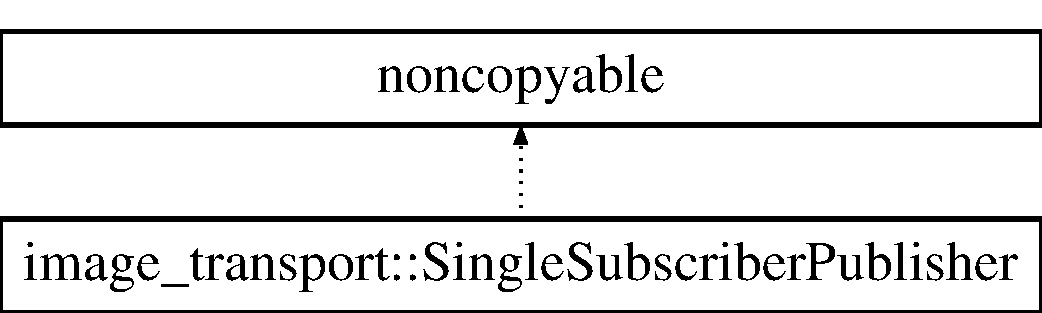
\includegraphics[height=2.000000cm]{classimage__transport_1_1_single_subscriber_publisher}
\end{center}
\end{figure}
\subsection*{Public Types}
\begin{DoxyCompactItemize}
\item 
\hypertarget{classimage__transport_1_1_single_subscriber_publisher_a30045c60864ff22374f025a81c2ca9cf}{typedef boost\-::function\\*
$<$ uint32\-\_\-t()$>$ {\bfseries Get\-Num\-Subscribers\-Fn}}\label{classimage__transport_1_1_single_subscriber_publisher_a30045c60864ff22374f025a81c2ca9cf}

\item 
\hypertarget{classimage__transport_1_1_single_subscriber_publisher_a83df64c8c339546b94b059314c73d939}{typedef boost\-::function$<$ void(const \\*
sensor\-\_\-msgs\-::\-Image \&)$>$ {\bfseries Publish\-Fn}}\label{classimage__transport_1_1_single_subscriber_publisher_a83df64c8c339546b94b059314c73d939}

\end{DoxyCompactItemize}
\subsection*{Public Member Functions}
\begin{DoxyCompactItemize}
\item 
\hypertarget{classimage__transport_1_1_single_subscriber_publisher_a4ed3520bfb119863c33890b1d3d76f7b}{{\bfseries Single\-Subscriber\-Publisher} (const std\-::string \&caller\-\_\-id, const std\-::string \&topic, const Get\-Num\-Subscribers\-Fn \&num\-\_\-subscribers\-\_\-fn, const Publish\-Fn \&publish\-\_\-fn)}\label{classimage__transport_1_1_single_subscriber_publisher_a4ed3520bfb119863c33890b1d3d76f7b}

\item 
\hypertarget{classimage__transport_1_1_single_subscriber_publisher_a1ddcc26cfb38ee6fec7bbc1e573d032d}{std\-::string {\bfseries get\-Subscriber\-Name} () const }\label{classimage__transport_1_1_single_subscriber_publisher_a1ddcc26cfb38ee6fec7bbc1e573d032d}

\item 
\hypertarget{classimage__transport_1_1_single_subscriber_publisher_a345d09ecd9691da5a215751dcde7c529}{std\-::string {\bfseries get\-Topic} () const }\label{classimage__transport_1_1_single_subscriber_publisher_a345d09ecd9691da5a215751dcde7c529}

\item 
\hypertarget{classimage__transport_1_1_single_subscriber_publisher_a5909a3e2feffe1abea5d0133a4d933a5}{uint32\-\_\-t {\bfseries get\-Num\-Subscribers} () const }\label{classimage__transport_1_1_single_subscriber_publisher_a5909a3e2feffe1abea5d0133a4d933a5}

\item 
\hypertarget{classimage__transport_1_1_single_subscriber_publisher_a6e5fb2d5f07e0b6e5fc7a67f7e733d58}{void {\bfseries publish} (const sensor\-\_\-msgs\-::\-Image \&message) const }\label{classimage__transport_1_1_single_subscriber_publisher_a6e5fb2d5f07e0b6e5fc7a67f7e733d58}

\item 
\hypertarget{classimage__transport_1_1_single_subscriber_publisher_a805ee398c71b942665f0e6a8878868f4}{void {\bfseries publish} (const sensor\-\_\-msgs\-::\-Image\-Const\-Ptr \&message) const }\label{classimage__transport_1_1_single_subscriber_publisher_a805ee398c71b942665f0e6a8878868f4}

\end{DoxyCompactItemize}
\subsection*{Friends}
\begin{DoxyCompactItemize}
\item 
\hypertarget{classimage__transport_1_1_single_subscriber_publisher_a9544c98126549cae8f3a5cd9af6bcfdd}{class {\bfseries Publisher}}\label{classimage__transport_1_1_single_subscriber_publisher_a9544c98126549cae8f3a5cd9af6bcfdd}

\end{DoxyCompactItemize}


\subsection{Detailed Description}
Allows publication of an image to a single subscriber. Only available inside subscriber connection callbacks. 

Definition at line 48 of file single\-\_\-subscriber\-\_\-publisher.\-h.



The documentation for this class was generated from the following files\-:\begin{DoxyCompactItemize}
\item 
/home/travis/catkin\-\_\-ws/src/image\-\_\-common/image\-\_\-transport/include/image\-\_\-transport/single\-\_\-subscriber\-\_\-publisher.\-h\item 
/home/travis/catkin\-\_\-ws/src/image\-\_\-common/image\-\_\-transport/src/single\-\_\-subscriber\-\_\-publisher.\-cpp\end{DoxyCompactItemize}

\hypertarget{classmsckf_1_1_state}{\section{msckf.\-State Class Reference}
\label{classmsckf_1_1_state}\index{msckf.\-State@{msckf.\-State}}
}
Inheritance diagram for msckf.\-State\-:\begin{figure}[H]
\begin{center}
\leavevmode
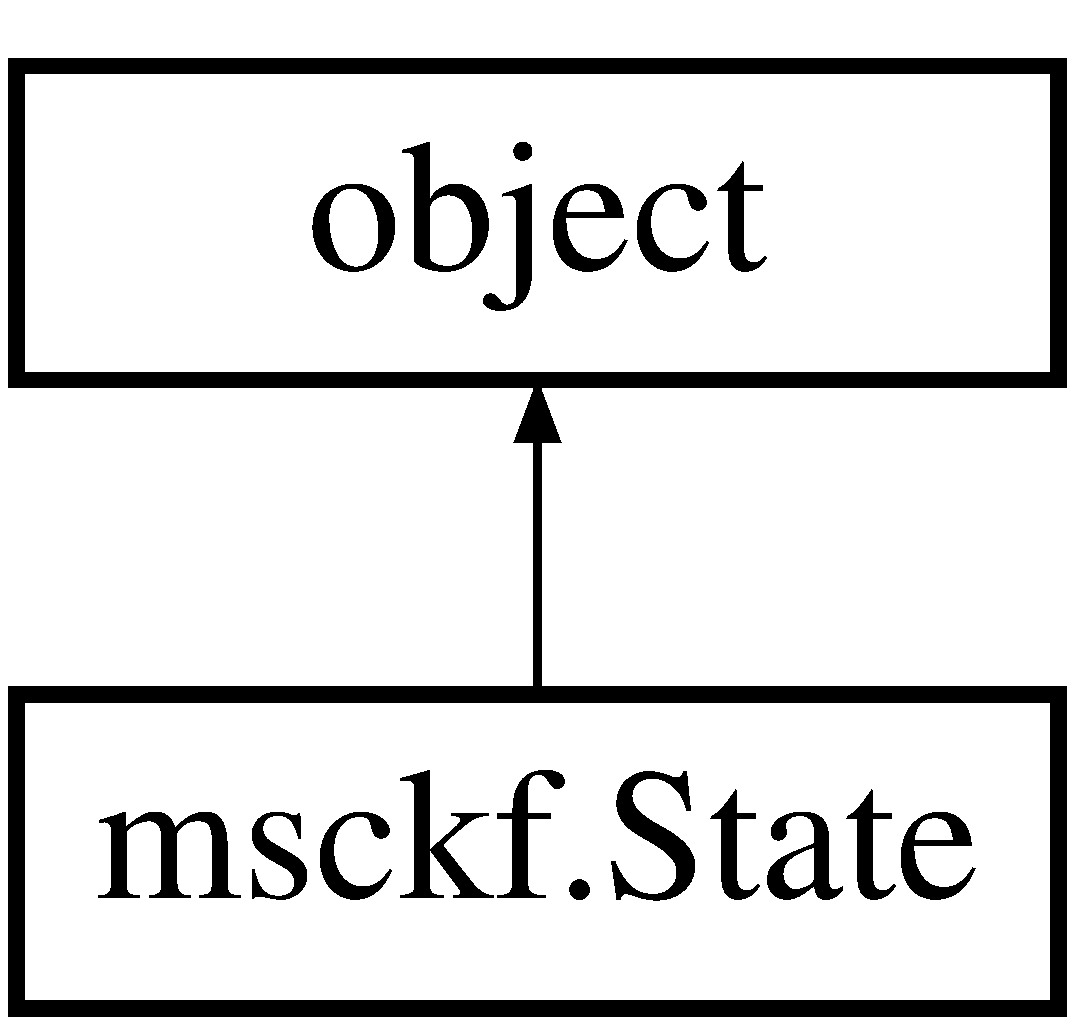
\includegraphics[height=2.000000cm]{classmsckf_1_1_state}
\end{center}
\end{figure}
\subsection*{Public Member Functions}
\begin{DoxyCompactItemize}
\item 
\hypertarget{classmsckf_1_1_state_a9eb4d9b6a0b22caf27964aae8321a8e4}{def {\bfseries \-\_\-\-\_\-init\-\_\-\-\_\-}}\label{classmsckf_1_1_state_a9eb4d9b6a0b22caf27964aae8321a8e4}

\item 
\hypertarget{classmsckf_1_1_state_ac6068aa29aaf8c12303feec1b194cee4}{def {\bfseries propagate}}\label{classmsckf_1_1_state_ac6068aa29aaf8c12303feec1b194cee4}

\item 
\hypertarget{classmsckf_1_1_state_acdb6b5075cf233ff40c38808a4e9b76f}{def {\bfseries initial\-\_\-attitude\-\_\-to\-\_\-empty\-\_\-state}}\label{classmsckf_1_1_state_acdb6b5075cf233ff40c38808a4e9b76f}

\item 
\hypertarget{classmsckf_1_1_state_a835e12a679c2dc50248383778bbb3d3b}{def {\bfseries estimate\-\_\-initial\-\_\-attitude}}\label{classmsckf_1_1_state_a835e12a679c2dc50248383778bbb3d3b}

\item 
\hypertarget{classmsckf_1_1_state_ae7c94f98c60ea6ed26d2fcf6e40d4d64}{def {\bfseries augment}}\label{classmsckf_1_1_state_ae7c94f98c60ea6ed26d2fcf6e40d4d64}

\item 
\hypertarget{classmsckf_1_1_state_a12ce863f430cec8c26e780341beffa81}{def {\bfseries remove\-\_\-n\-\_\-cam\-\_\-poses}}\label{classmsckf_1_1_state_a12ce863f430cec8c26e780341beffa81}

\item 
\hypertarget{classmsckf_1_1_state_a4e782e52dd630137558f15c5c3ef0a93}{def {\bfseries get\-\_\-pose\-\_\-to\-\_\-pose\-\_\-rotation}}\label{classmsckf_1_1_state_a4e782e52dd630137558f15c5c3ef0a93}

\item 
\hypertarget{classmsckf_1_1_state_a8aa0ea4bfcb8f10a26210779211bc72c}{def {\bfseries get\-\_\-position\-\_\-of\-\_\-pose\-\_\-in\-\_\-another\-\_\-pose}}\label{classmsckf_1_1_state_a8aa0ea4bfcb8f10a26210779211bc72c}

\item 
\hypertarget{classmsckf_1_1_state_a675ba96049a53a5b524ec12d6b1db492}{def {\bfseries get\-\_\-rotation\-\_\-from\-\_\-global\-\_\-to\-\_\-camera\-\_\-pose}}\label{classmsckf_1_1_state_a675ba96049a53a5b524ec12d6b1db492}

\item 
\hypertarget{classmsckf_1_1_state_a4d73be1dbaa64387ab9914166a1911c7}{def {\bfseries get\-\_\-position\-\_\-of\-\_\-pose\-\_\-in\-\_\-global\-\_\-frame}}\label{classmsckf_1_1_state_a4d73be1dbaa64387ab9914166a1911c7}

\item 
\hypertarget{classmsckf_1_1_state_a2a4bea03daac8393f9e79478cb1cfc9c}{def {\bfseries time\-\_\-to}}\label{classmsckf_1_1_state_a2a4bea03daac8393f9e79478cb1cfc9c}

\item 
\hypertarget{classmsckf_1_1_state_a87fac63716f6150b0389e14ba5b4f740}{def {\bfseries compute\-\_\-rotation\-\_\-estimate}}\label{classmsckf_1_1_state_a87fac63716f6150b0389e14ba5b4f740}

\item 
\hypertarget{classmsckf_1_1_state_ab3159f30af3ec38d872f93292a9676ab}{def {\bfseries compute\-\_\-acceleration\-\_\-estimate}}\label{classmsckf_1_1_state_ab3159f30af3ec38d872f93292a9676ab}

\end{DoxyCompactItemize}
\subsection*{Static Public Member Functions}
\begin{DoxyCompactItemize}
\item 
\hypertarget{classmsckf_1_1_state_af4664b6f5c6b28f190702944cea1b206}{def {\bfseries get\-\_\-body\-\_\-to\-\_\-camera\-\_\-frame\-\_\-rotation}}\label{classmsckf_1_1_state_af4664b6f5c6b28f190702944cea1b206}

\end{DoxyCompactItemize}
\subsection*{Public Attributes}
\begin{DoxyCompactItemize}
\item 
\hypertarget{classmsckf_1_1_state_a4685283913afe8e3762f885b1ee49aaa}{{\bfseries b\-\_\-g}}\label{classmsckf_1_1_state_a4685283913afe8e3762f885b1ee49aaa}

\item 
\hypertarget{classmsckf_1_1_state_ab5334519dab92512663743a21325b6d0}{{\bfseries b\-\_\-a}}\label{classmsckf_1_1_state_ab5334519dab92512663743a21325b6d0}

\item 
\hypertarget{classmsckf_1_1_state_acb42c97d2bc8b414e1d123c32d3bce7b}{{\bfseries T\-\_\-g}}\label{classmsckf_1_1_state_acb42c97d2bc8b414e1d123c32d3bce7b}

\item 
\hypertarget{classmsckf_1_1_state_a55f507697e1df1dc272c3b394c98a594}{{\bfseries T\-\_\-s}}\label{classmsckf_1_1_state_a55f507697e1df1dc272c3b394c98a594}

\item 
\hypertarget{classmsckf_1_1_state_ac10d747d657c748a00dec2fadf730cd4}{{\bfseries T\-\_\-a}}\label{classmsckf_1_1_state_ac10d747d657c748a00dec2fadf730cd4}

\item 
\hypertarget{classmsckf_1_1_state_afea15c330a8f44f4081d612fcf5aaca7}{{\bfseries p\-\_\-\-B\-\_\-\-C}}\label{classmsckf_1_1_state_afea15c330a8f44f4081d612fcf5aaca7}

\item 
\hypertarget{classmsckf_1_1_state_a27095fe241e9cb72ada586d442d6a143}{{\bfseries f\-\_\-y}}\label{classmsckf_1_1_state_a27095fe241e9cb72ada586d442d6a143}

\item 
\hypertarget{classmsckf_1_1_state_aba04b13698fdc6cfe7c2d32324432459}{{\bfseries o\-\_\-y}}\label{classmsckf_1_1_state_aba04b13698fdc6cfe7c2d32324432459}

\item 
\hypertarget{classmsckf_1_1_state_ac35ee5c42c4a17b9a219b811b47a876f}{{\bfseries k\-\_\-3}}\label{classmsckf_1_1_state_ac35ee5c42c4a17b9a219b811b47a876f}

\item 
\hypertarget{classmsckf_1_1_state_ae553c742f849304bb8514981a499389c}{{\bfseries t\-\_\-2}}\label{classmsckf_1_1_state_ae553c742f849304bb8514981a499389c}

\item 
\hypertarget{classmsckf_1_1_state_a6a576f30d3a2f42f29adc87e03dd0876}{{\bfseries t\-\_\-r}}\label{classmsckf_1_1_state_a6a576f30d3a2f42f29adc87e03dd0876}

\item 
\hypertarget{classmsckf_1_1_state_a3e5e50676def313ecdc9ba6b0878b039}{{\bfseries body\-\_\-state}}\label{classmsckf_1_1_state_a3e5e50676def313ecdc9ba6b0878b039}

\item 
\hypertarget{classmsckf_1_1_state_a1e93e259f7390bba92ef3f2445aa2112}{{\bfseries sigma}}\label{classmsckf_1_1_state_a1e93e259f7390bba92ef3f2445aa2112}

\item 
\hypertarget{classmsckf_1_1_state_a6c6b64481b9d723a74afd5b521941c90}{{\bfseries camera\-\_\-poses}}\label{classmsckf_1_1_state_a6c6b64481b9d723a74afd5b521941c90}

\item 
\hypertarget{classmsckf_1_1_state_a28ba89e11bae7d996ff4218c826bf376}{{\bfseries features\-\_\-tracked\-\_\-in\-\_\-image}}\label{classmsckf_1_1_state_a28ba89e11bae7d996ff4218c826bf376}

\item 
\hypertarget{classmsckf_1_1_state_a7b6759e1c42e803e7f9d6a97079c3ec1}{{\bfseries first\-\_\-camera\-\_\-pose\-\_\-id}}\label{classmsckf_1_1_state_a7b6759e1c42e803e7f9d6a97079c3ec1}

\item 
\hypertarget{classmsckf_1_1_state_ae460a78ec25da8e33378372a2dc9943c}{{\bfseries past\-\_\-last\-\_\-camera\-\_\-pose\-\_\-id}}\label{classmsckf_1_1_state_ae460a78ec25da8e33378372a2dc9943c}

\end{DoxyCompactItemize}
\subsection*{Properties}
\begin{DoxyCompactItemize}
\item 
\hypertarget{classmsckf_1_1_state_abde5f106d34d598e79e5130308fd9103}{{\bfseries time} = property(lambda self\-: self.\-body\-\_\-state.\-time)}\label{classmsckf_1_1_state_abde5f106d34d598e79e5130308fd9103}

\item 
\hypertarget{classmsckf_1_1_state_aa0757a330d508319925982feed2f20a9}{{\bfseries q\-\_\-\-B\-\_\-\-G} = property(lambda self\-: self.\-body\-\_\-state.\-q\-\_\-\-B\-\_\-\-G)}\label{classmsckf_1_1_state_aa0757a330d508319925982feed2f20a9}

\item 
\hypertarget{classmsckf_1_1_state_a44862ee855b4fcedd843693f33932374}{{\bfseries p\-\_\-\-B\-\_\-\-G} = property(lambda self\-: self.\-body\-\_\-state.\-p\-\_\-\-B\-\_\-\-G)}\label{classmsckf_1_1_state_a44862ee855b4fcedd843693f33932374}

\item 
\hypertarget{classmsckf_1_1_state_a4a626bb3ecffdbc910bde67231f5825e}{{\bfseries v\-\_\-\-B\-\_\-\-G} = property(lambda self\-: self.\-body\-\_\-state.\-v\-\_\-\-B\-\_\-\-G)}\label{classmsckf_1_1_state_a4a626bb3ecffdbc910bde67231f5825e}

\item 
\hypertarget{classmsckf_1_1_state_ac75587b0f3c1c263d063e437d75a5384}{{\bfseries pose} = property(lambda self\-: \hyperlink{classmsckf_1_1_pose_get}{Pose\-Get}(self))}\label{classmsckf_1_1_state_ac75587b0f3c1c263d063e437d75a5384}

\end{DoxyCompactItemize}


\subsection{Detailed Description}


Definition at line 319 of file msckf.\-py.



The documentation for this class was generated from the following file\-:\begin{DoxyCompactItemize}
\item 
/home/travis/build/tomas789/tonav/prototype/msckf.\-py\end{DoxyCompactItemize}

\hypertarget{classimage__transport_1_1_subscriber}{\section{image\-\_\-transport\-:\-:Subscriber Class Reference}
\label{classimage__transport_1_1_subscriber}\index{image\-\_\-transport\-::\-Subscriber@{image\-\_\-transport\-::\-Subscriber}}
}


Manages a subscription callback on a specific topic that can be interpreted as an Image topic.  




{\ttfamily \#include $<$subscriber.\-h$>$}

\subsection*{Classes}
\begin{DoxyCompactItemize}
\item 
struct \hyperlink{structimage__transport_1_1_subscriber_1_1_impl}{Impl}
\end{DoxyCompactItemize}
\subsection*{Public Member Functions}
\begin{DoxyCompactItemize}
\item 
std\-::string \hyperlink{classimage__transport_1_1_subscriber_ae8d6676e24bb42dd4b57484db5770c1b}{get\-Topic} () const 
\begin{DoxyCompactList}\small\item\em Returns the base image topic. \end{DoxyCompactList}\item 
\hypertarget{classimage__transport_1_1_subscriber_ac5b0836c603afc1faa961bbf279e48da}{uint32\-\_\-t \hyperlink{classimage__transport_1_1_subscriber_ac5b0836c603afc1faa961bbf279e48da}{get\-Num\-Publishers} () const }\label{classimage__transport_1_1_subscriber_ac5b0836c603afc1faa961bbf279e48da}

\begin{DoxyCompactList}\small\item\em Returns the number of publishers this subscriber is connected to. \end{DoxyCompactList}\item 
\hypertarget{classimage__transport_1_1_subscriber_ac1b8ae33bf243c09e33e293330a2a4b7}{std\-::string \hyperlink{classimage__transport_1_1_subscriber_ac1b8ae33bf243c09e33e293330a2a4b7}{get\-Transport} () const }\label{classimage__transport_1_1_subscriber_ac1b8ae33bf243c09e33e293330a2a4b7}

\begin{DoxyCompactList}\small\item\em Returns the name of the transport being used. \end{DoxyCompactList}\item 
\hypertarget{classimage__transport_1_1_subscriber_a014af7126efc24adf6dc4d11ac9bca6b}{void \hyperlink{classimage__transport_1_1_subscriber_a014af7126efc24adf6dc4d11ac9bca6b}{shutdown} ()}\label{classimage__transport_1_1_subscriber_a014af7126efc24adf6dc4d11ac9bca6b}

\begin{DoxyCompactList}\small\item\em Unsubscribe the callback associated with this \hyperlink{classimage__transport_1_1_subscriber}{Subscriber}. \end{DoxyCompactList}\item 
\hypertarget{classimage__transport_1_1_subscriber_a23659b0b3552134bf47af54e847b6063}{{\bfseries operator void $\ast$} () const }\label{classimage__transport_1_1_subscriber_a23659b0b3552134bf47af54e847b6063}

\item 
\hypertarget{classimage__transport_1_1_subscriber_aec02fe5a92183fb63e94b0c70739d363}{bool {\bfseries operator$<$} (const \hyperlink{classimage__transport_1_1_subscriber}{Subscriber} \&rhs) const }\label{classimage__transport_1_1_subscriber_aec02fe5a92183fb63e94b0c70739d363}

\item 
\hypertarget{classimage__transport_1_1_subscriber_a30e373deed0ab800184c5d2c7bac2dba}{bool {\bfseries operator!=} (const \hyperlink{classimage__transport_1_1_subscriber}{Subscriber} \&rhs) const }\label{classimage__transport_1_1_subscriber_a30e373deed0ab800184c5d2c7bac2dba}

\item 
\hypertarget{classimage__transport_1_1_subscriber_a6428c74a8fc9cabcac2e9f11c50f25cf}{bool {\bfseries operator==} (const \hyperlink{classimage__transport_1_1_subscriber}{Subscriber} \&rhs) const }\label{classimage__transport_1_1_subscriber_a6428c74a8fc9cabcac2e9f11c50f25cf}

\end{DoxyCompactItemize}
\subsection*{Friends}
\begin{DoxyCompactItemize}
\item 
\hypertarget{classimage__transport_1_1_subscriber_ac010f5a40d98825199e1c5303d0638eb}{class {\bfseries Image\-Transport}}\label{classimage__transport_1_1_subscriber_ac010f5a40d98825199e1c5303d0638eb}

\end{DoxyCompactItemize}


\subsection{Detailed Description}
Manages a subscription callback on a specific topic that can be interpreted as an Image topic. 

\hyperlink{classimage__transport_1_1_subscriber}{Subscriber} is the client-\/side counterpart to \hyperlink{classimage__transport_1_1_publisher}{Publisher}. By loading the appropriate plugin, it can subscribe to a base image topic using any available transport. The complexity of what transport is actually used is hidden from the user, who sees only a normal Image callback.

A \hyperlink{classimage__transport_1_1_subscriber}{Subscriber} should always be created through a call to \hyperlink{classimage__transport_1_1_image_transport_a1c847a2c719c874f84a78a6a60b98c7f}{Image\-Transport\-::subscribe()}, or copied from one that was. Once all copies of a specific \hyperlink{classimage__transport_1_1_subscriber}{Subscriber} go out of scope, the subscription callback associated with that handle will stop being called. Once all \hyperlink{classimage__transport_1_1_subscriber}{Subscriber} for a given topic go out of scope the topic will be unsubscribed. 

Definition at line 61 of file subscriber.\-h.



\subsection{Member Function Documentation}
\hypertarget{classimage__transport_1_1_subscriber_ae8d6676e24bb42dd4b57484db5770c1b}{\index{image\-\_\-transport\-::\-Subscriber@{image\-\_\-transport\-::\-Subscriber}!get\-Topic@{get\-Topic}}
\index{get\-Topic@{get\-Topic}!image_transport::Subscriber@{image\-\_\-transport\-::\-Subscriber}}
\subsubsection[{get\-Topic}]{\setlength{\rightskip}{0pt plus 5cm}std\-::string image\-\_\-transport\-::\-Subscriber\-::get\-Topic (
\begin{DoxyParamCaption}
{}
\end{DoxyParamCaption}
) const}}\label{classimage__transport_1_1_subscriber_ae8d6676e24bb42dd4b57484db5770c1b}


Returns the base image topic. 

The \hyperlink{classimage__transport_1_1_subscriber}{Subscriber} may actually be subscribed to some transport-\/specific topic that differs from the base topic. 

Definition at line 114 of file subscriber.\-cpp.



The documentation for this class was generated from the following files\-:\begin{DoxyCompactItemize}
\item 
/home/travis/catkin\-\_\-ws/src/image\-\_\-common/image\-\_\-transport/include/image\-\_\-transport/subscriber.\-h\item 
/home/travis/catkin\-\_\-ws/src/image\-\_\-common/image\-\_\-transport/src/subscriber.\-cpp\end{DoxyCompactItemize}

\hypertarget{classimage__transport_1_1_subscriber_filter}{\section{image\-\_\-transport\-:\-:Subscriber\-Filter Class Reference}
\label{classimage__transport_1_1_subscriber_filter}\index{image\-\_\-transport\-::\-Subscriber\-Filter@{image\-\_\-transport\-::\-Subscriber\-Filter}}
}


Image subscription filter.  




{\ttfamily \#include $<$subscriber\-\_\-filter.\-h$>$}

Inheritance diagram for image\-\_\-transport\-:\-:Subscriber\-Filter\-:\begin{figure}[H]
\begin{center}
\leavevmode
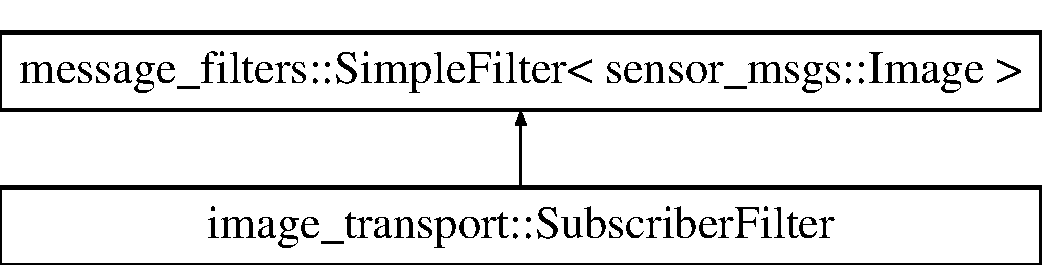
\includegraphics[height=2.000000cm]{classimage__transport_1_1_subscriber_filter}
\end{center}
\end{figure}
\subsection*{Public Member Functions}
\begin{DoxyCompactItemize}
\item 
\hyperlink{classimage__transport_1_1_subscriber_filter_afae6f86755c38b573bc5fa35e43e37f3}{Subscriber\-Filter} (\hyperlink{classimage__transport_1_1_image_transport}{Image\-Transport} \&it, const std\-::string \&base\-\_\-topic, uint32\-\_\-t queue\-\_\-size, const \hyperlink{classimage__transport_1_1_transport_hints}{Transport\-Hints} \&transport\-\_\-hints=\hyperlink{classimage__transport_1_1_transport_hints}{Transport\-Hints}())
\begin{DoxyCompactList}\small\item\em Constructor. \end{DoxyCompactList}\item 
\hypertarget{classimage__transport_1_1_subscriber_filter_a2378a43c41e4fe123193ca637eb49afd}{\hyperlink{classimage__transport_1_1_subscriber_filter_a2378a43c41e4fe123193ca637eb49afd}{Subscriber\-Filter} ()}\label{classimage__transport_1_1_subscriber_filter_a2378a43c41e4fe123193ca637eb49afd}

\begin{DoxyCompactList}\small\item\em Empty constructor, use \hyperlink{classimage__transport_1_1_subscriber_filter_a20afdaa28a22ffdbf62226ba1c95e561}{subscribe()} to subscribe to a topic. \end{DoxyCompactList}\item 
void \hyperlink{classimage__transport_1_1_subscriber_filter_a20afdaa28a22ffdbf62226ba1c95e561}{subscribe} (\hyperlink{classimage__transport_1_1_image_transport}{Image\-Transport} \&it, const std\-::string \&base\-\_\-topic, uint32\-\_\-t queue\-\_\-size, const \hyperlink{classimage__transport_1_1_transport_hints}{Transport\-Hints} \&transport\-\_\-hints=\hyperlink{classimage__transport_1_1_transport_hints}{Transport\-Hints}())
\begin{DoxyCompactList}\small\item\em Subscribe to a topic. \end{DoxyCompactList}\item 
\hypertarget{classimage__transport_1_1_subscriber_filter_a058bfa4c200c90d7cabd18a2d674084b}{void \hyperlink{classimage__transport_1_1_subscriber_filter_a058bfa4c200c90d7cabd18a2d674084b}{unsubscribe} ()}\label{classimage__transport_1_1_subscriber_filter_a058bfa4c200c90d7cabd18a2d674084b}

\begin{DoxyCompactList}\small\item\em Force immediate unsubscription of this subscriber from its topic. \end{DoxyCompactList}\item 
\hypertarget{classimage__transport_1_1_subscriber_filter_a9579b79c3a19cfcbd84586efddad52d5}{std\-::string {\bfseries get\-Topic} () const }\label{classimage__transport_1_1_subscriber_filter_a9579b79c3a19cfcbd84586efddad52d5}

\item 
\hypertarget{classimage__transport_1_1_subscriber_filter_abebc23b9066f8c684a1ce6d3906d5f99}{uint32\-\_\-t \hyperlink{classimage__transport_1_1_subscriber_filter_abebc23b9066f8c684a1ce6d3906d5f99}{get\-Num\-Publishers} () const }\label{classimage__transport_1_1_subscriber_filter_abebc23b9066f8c684a1ce6d3906d5f99}

\begin{DoxyCompactList}\small\item\em Returns the number of publishers this subscriber is connected to. \end{DoxyCompactList}\item 
\hypertarget{classimage__transport_1_1_subscriber_filter_a9ba5a0e16e68dc055e0e4aba9679a281}{std\-::string \hyperlink{classimage__transport_1_1_subscriber_filter_a9ba5a0e16e68dc055e0e4aba9679a281}{get\-Transport} () const }\label{classimage__transport_1_1_subscriber_filter_a9ba5a0e16e68dc055e0e4aba9679a281}

\begin{DoxyCompactList}\small\item\em Returns the name of the transport being used. \end{DoxyCompactList}\item 
\hypertarget{classimage__transport_1_1_subscriber_filter_ab0fdf78b86de2231788b74a911892d4c}{const \hyperlink{classimage__transport_1_1_subscriber}{Subscriber} \& \hyperlink{classimage__transport_1_1_subscriber_filter_ab0fdf78b86de2231788b74a911892d4c}{get\-Subscriber} () const }\label{classimage__transport_1_1_subscriber_filter_ab0fdf78b86de2231788b74a911892d4c}

\begin{DoxyCompactList}\small\item\em Returns the internal \hyperlink{classimage__transport_1_1_subscriber}{image\-\_\-transport\-::\-Subscriber} object. \end{DoxyCompactList}\end{DoxyCompactItemize}


\subsection{Detailed Description}
Image subscription filter. 

This class wraps \hyperlink{classimage__transport_1_1_subscriber}{Subscriber} as a \char`\"{}filter\char`\"{} compatible with the message\-\_\-filters package. It acts as a highest-\/level filter, simply passing messages from an image transport subscription through to the filters which have connected to it.

When this object is destroyed it will unsubscribe from the R\-O\-S subscription.\hypertarget{classimage__transport_1_1_subscriber_filter_connections}{}\subsection{C\-O\-N\-N\-E\-C\-T\-I\-O\-N\-S}\label{classimage__transport_1_1_subscriber_filter_connections}
\hyperlink{classimage__transport_1_1_subscriber_filter}{Subscriber\-Filter} has no input connection.

The output connection for the \hyperlink{classimage__transport_1_1_subscriber_filter}{Subscriber\-Filter} object is the same signature as for roscpp subscription callbacks, ie. \begin{DoxyVerb}void callback(const boost::shared_ptr<const sensor_msgs::Image>&);
\end{DoxyVerb}
 

Definition at line 64 of file subscriber\-\_\-filter.\-h.



\subsection{Constructor \& Destructor Documentation}
\hypertarget{classimage__transport_1_1_subscriber_filter_afae6f86755c38b573bc5fa35e43e37f3}{\index{image\-\_\-transport\-::\-Subscriber\-Filter@{image\-\_\-transport\-::\-Subscriber\-Filter}!Subscriber\-Filter@{Subscriber\-Filter}}
\index{Subscriber\-Filter@{Subscriber\-Filter}!image_transport::SubscriberFilter@{image\-\_\-transport\-::\-Subscriber\-Filter}}
\subsubsection[{Subscriber\-Filter}]{\setlength{\rightskip}{0pt plus 5cm}image\-\_\-transport\-::\-Subscriber\-Filter\-::\-Subscriber\-Filter (
\begin{DoxyParamCaption}
\item[{{\bf Image\-Transport} \&}]{it, }
\item[{const std\-::string \&}]{base\-\_\-topic, }
\item[{uint32\-\_\-t}]{queue\-\_\-size, }
\item[{const {\bf Transport\-Hints} \&}]{transport\-\_\-hints = {\ttfamily {\bf Transport\-Hints}()}}
\end{DoxyParamCaption}
)\hspace{0.3cm}{\ttfamily [inline]}}}\label{classimage__transport_1_1_subscriber_filter_afae6f86755c38b573bc5fa35e43e37f3}


Constructor. 

See the ros\-::\-Node\-Handle\-::subscribe() variants for more information on the parameters


\begin{DoxyParams}{Parameters}
{\em nh} & The ros\-::\-Node\-Handle to use to subscribe. \\
\hline
{\em base\-\_\-topic} & The topic to subscribe to. \\
\hline
{\em queue\-\_\-size} & The subscription queue size \\
\hline
{\em transport\-\_\-hints} & The transport hints to pass along \\
\hline
\end{DoxyParams}


Definition at line 77 of file subscriber\-\_\-filter.\-h.



\subsection{Member Function Documentation}
\hypertarget{classimage__transport_1_1_subscriber_filter_a20afdaa28a22ffdbf62226ba1c95e561}{\index{image\-\_\-transport\-::\-Subscriber\-Filter@{image\-\_\-transport\-::\-Subscriber\-Filter}!subscribe@{subscribe}}
\index{subscribe@{subscribe}!image_transport::SubscriberFilter@{image\-\_\-transport\-::\-Subscriber\-Filter}}
\subsubsection[{subscribe}]{\setlength{\rightskip}{0pt plus 5cm}void image\-\_\-transport\-::\-Subscriber\-Filter\-::subscribe (
\begin{DoxyParamCaption}
\item[{{\bf Image\-Transport} \&}]{it, }
\item[{const std\-::string \&}]{base\-\_\-topic, }
\item[{uint32\-\_\-t}]{queue\-\_\-size, }
\item[{const {\bf Transport\-Hints} \&}]{transport\-\_\-hints = {\ttfamily {\bf Transport\-Hints}()}}
\end{DoxyParamCaption}
)\hspace{0.3cm}{\ttfamily [inline]}}}\label{classimage__transport_1_1_subscriber_filter_a20afdaa28a22ffdbf62226ba1c95e561}


Subscribe to a topic. 

If this \hyperlink{classimage__transport_1_1_subscriber}{Subscriber} is already subscribed to a topic, this function will first unsubscribe.


\begin{DoxyParams}{Parameters}
{\em nh} & The ros\-::\-Node\-Handle to use to subscribe. \\
\hline
{\em base\-\_\-topic} & The topic to subscribe to. \\
\hline
{\em queue\-\_\-size} & The subscription queue size \\
\hline
{\em transport\-\_\-hints} & The transport hints to pass along \\
\hline
\end{DoxyParams}


Definition at line 105 of file subscriber\-\_\-filter.\-h.



The documentation for this class was generated from the following file\-:\begin{DoxyCompactItemize}
\item 
/home/travis/catkin\-\_\-ws/src/image\-\_\-common/image\-\_\-transport/include/image\-\_\-transport/subscriber\-\_\-filter.\-h\end{DoxyCompactItemize}

\hypertarget{classimage__transport_1_1_subscriber_plugin}{\section{image\-\_\-transport\-:\-:Subscriber\-Plugin Class Reference}
\label{classimage__transport_1_1_subscriber_plugin}\index{image\-\_\-transport\-::\-Subscriber\-Plugin@{image\-\_\-transport\-::\-Subscriber\-Plugin}}
}


Base class for plugins to \hyperlink{classimage__transport_1_1_subscriber}{Subscriber}.  




{\ttfamily \#include $<$subscriber\-\_\-plugin.\-h$>$}

Inheritance diagram for image\-\_\-transport\-:\-:Subscriber\-Plugin\-:\begin{figure}[H]
\begin{center}
\leavevmode
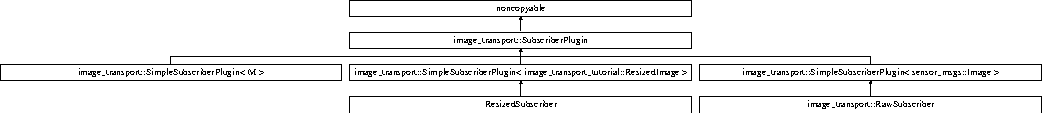
\includegraphics[height=1.517615cm]{classimage__transport_1_1_subscriber_plugin}
\end{center}
\end{figure}
\subsection*{Public Types}
\begin{DoxyCompactItemize}
\item 
\hypertarget{classimage__transport_1_1_subscriber_plugin_a0e3d423158a12f55e528b108d6dfda19}{typedef boost\-::function$<$ void(const \\*
sensor\-\_\-msgs\-::\-Image\-Const\-Ptr \&)$>$ {\bfseries Callback}}\label{classimage__transport_1_1_subscriber_plugin_a0e3d423158a12f55e528b108d6dfda19}

\end{DoxyCompactItemize}
\subsection*{Public Member Functions}
\begin{DoxyCompactItemize}
\item 
\hypertarget{classimage__transport_1_1_subscriber_plugin_a647dc0f6e0c34f0b4d8b809b3c679f88}{virtual std\-::string \hyperlink{classimage__transport_1_1_subscriber_plugin_a647dc0f6e0c34f0b4d8b809b3c679f88}{get\-Transport\-Name} () const =0}\label{classimage__transport_1_1_subscriber_plugin_a647dc0f6e0c34f0b4d8b809b3c679f88}

\begin{DoxyCompactList}\small\item\em Get a string identifier for the transport provided by this plugin. \end{DoxyCompactList}\item 
\hypertarget{classimage__transport_1_1_subscriber_plugin_abf53246a79405014beab159908a11ec8}{void \hyperlink{classimage__transport_1_1_subscriber_plugin_abf53246a79405014beab159908a11ec8}{subscribe} (ros\-::\-Node\-Handle \&nh, const std\-::string \&base\-\_\-topic, uint32\-\_\-t queue\-\_\-size, const Callback \&callback, const ros\-::\-Void\-Ptr \&tracked\-\_\-object=ros\-::\-Void\-Ptr(), const \hyperlink{classimage__transport_1_1_transport_hints}{Transport\-Hints} \&transport\-\_\-hints=\hyperlink{classimage__transport_1_1_transport_hints}{Transport\-Hints}())}\label{classimage__transport_1_1_subscriber_plugin_abf53246a79405014beab159908a11ec8}

\begin{DoxyCompactList}\small\item\em Subscribe to an image topic, version for arbitrary boost\-::function object. \end{DoxyCompactList}\item 
\hypertarget{classimage__transport_1_1_subscriber_plugin_a699938e88a295ad3ae6d770fceb41690}{void \hyperlink{classimage__transport_1_1_subscriber_plugin_a699938e88a295ad3ae6d770fceb41690}{subscribe} (ros\-::\-Node\-Handle \&nh, const std\-::string \&base\-\_\-topic, uint32\-\_\-t queue\-\_\-size, void($\ast$fp)(const sensor\-\_\-msgs\-::\-Image\-Const\-Ptr \&), const \hyperlink{classimage__transport_1_1_transport_hints}{Transport\-Hints} \&transport\-\_\-hints=\hyperlink{classimage__transport_1_1_transport_hints}{Transport\-Hints}())}\label{classimage__transport_1_1_subscriber_plugin_a699938e88a295ad3ae6d770fceb41690}

\begin{DoxyCompactList}\small\item\em Subscribe to an image topic, version for bare function. \end{DoxyCompactList}\item 
\hypertarget{classimage__transport_1_1_subscriber_plugin_a9cd92f4bac80d9f89d949082581ad4fe}{{\footnotesize template$<$class T $>$ }\\void \hyperlink{classimage__transport_1_1_subscriber_plugin_a9cd92f4bac80d9f89d949082581ad4fe}{subscribe} (ros\-::\-Node\-Handle \&nh, const std\-::string \&base\-\_\-topic, uint32\-\_\-t queue\-\_\-size, void(T\-::$\ast$fp)(const sensor\-\_\-msgs\-::\-Image\-Const\-Ptr \&), T $\ast$obj, const \hyperlink{classimage__transport_1_1_transport_hints}{Transport\-Hints} \&transport\-\_\-hints=\hyperlink{classimage__transport_1_1_transport_hints}{Transport\-Hints}())}\label{classimage__transport_1_1_subscriber_plugin_a9cd92f4bac80d9f89d949082581ad4fe}

\begin{DoxyCompactList}\small\item\em Subscribe to an image topic, version for class member function with bare pointer. \end{DoxyCompactList}\item 
\hypertarget{classimage__transport_1_1_subscriber_plugin_acb23bea81d54ee21cd5fa12ddd871aaa}{{\footnotesize template$<$class T $>$ }\\void \hyperlink{classimage__transport_1_1_subscriber_plugin_acb23bea81d54ee21cd5fa12ddd871aaa}{subscribe} (ros\-::\-Node\-Handle \&nh, const std\-::string \&base\-\_\-topic, uint32\-\_\-t queue\-\_\-size, void(T\-::$\ast$fp)(const sensor\-\_\-msgs\-::\-Image\-Const\-Ptr \&), const boost\-::shared\-\_\-ptr$<$ T $>$ \&obj, const \hyperlink{classimage__transport_1_1_transport_hints}{Transport\-Hints} \&transport\-\_\-hints=\hyperlink{classimage__transport_1_1_transport_hints}{Transport\-Hints}())}\label{classimage__transport_1_1_subscriber_plugin_acb23bea81d54ee21cd5fa12ddd871aaa}

\begin{DoxyCompactList}\small\item\em Subscribe to an image topic, version for class member function with shared\-\_\-ptr. \end{DoxyCompactList}\item 
\hypertarget{classimage__transport_1_1_subscriber_plugin_abb289f564cb993a990626662e65bd9f6}{virtual std\-::string \hyperlink{classimage__transport_1_1_subscriber_plugin_abb289f564cb993a990626662e65bd9f6}{get\-Topic} () const =0}\label{classimage__transport_1_1_subscriber_plugin_abb289f564cb993a990626662e65bd9f6}

\begin{DoxyCompactList}\small\item\em Get the transport-\/specific communication topic. \end{DoxyCompactList}\item 
\hypertarget{classimage__transport_1_1_subscriber_plugin_a7fae40b302a6493d00b0cd8905484677}{virtual uint32\-\_\-t \hyperlink{classimage__transport_1_1_subscriber_plugin_a7fae40b302a6493d00b0cd8905484677}{get\-Num\-Publishers} () const =0}\label{classimage__transport_1_1_subscriber_plugin_a7fae40b302a6493d00b0cd8905484677}

\begin{DoxyCompactList}\small\item\em Returns the number of publishers this subscriber is connected to. \end{DoxyCompactList}\item 
\hypertarget{classimage__transport_1_1_subscriber_plugin_aa8af1348748aef7372bf248a69f775a7}{virtual void \hyperlink{classimage__transport_1_1_subscriber_plugin_aa8af1348748aef7372bf248a69f775a7}{shutdown} ()=0}\label{classimage__transport_1_1_subscriber_plugin_aa8af1348748aef7372bf248a69f775a7}

\begin{DoxyCompactList}\small\item\em Unsubscribe the callback associated with this \hyperlink{classimage__transport_1_1_subscriber_plugin}{Subscriber\-Plugin}. \end{DoxyCompactList}\end{DoxyCompactItemize}
\subsection*{Static Public Member Functions}
\begin{DoxyCompactItemize}
\item 
\hypertarget{classimage__transport_1_1_subscriber_plugin_ae48e1648e998fe8352ff385c4c132531}{static std\-::string \hyperlink{classimage__transport_1_1_subscriber_plugin_ae48e1648e998fe8352ff385c4c132531}{get\-Lookup\-Name} (const std\-::string \&transport\-\_\-type)}\label{classimage__transport_1_1_subscriber_plugin_ae48e1648e998fe8352ff385c4c132531}

\begin{DoxyCompactList}\small\item\em Return the lookup name of the \hyperlink{classimage__transport_1_1_subscriber_plugin}{Subscriber\-Plugin} associated with a specific transport identifier. \end{DoxyCompactList}\end{DoxyCompactItemize}
\subsection*{Protected Member Functions}
\begin{DoxyCompactItemize}
\item 
\hypertarget{classimage__transport_1_1_subscriber_plugin_a1cc8b28b99ea0a15c9e58dc6d9bc27f6}{virtual void \hyperlink{classimage__transport_1_1_subscriber_plugin_a1cc8b28b99ea0a15c9e58dc6d9bc27f6}{subscribe\-Impl} (ros\-::\-Node\-Handle \&nh, const std\-::string \&base\-\_\-topic, uint32\-\_\-t queue\-\_\-size, const Callback \&callback, const ros\-::\-Void\-Ptr \&tracked\-\_\-object, const \hyperlink{classimage__transport_1_1_transport_hints}{Transport\-Hints} \&transport\-\_\-hints)=0}\label{classimage__transport_1_1_subscriber_plugin_a1cc8b28b99ea0a15c9e58dc6d9bc27f6}

\begin{DoxyCompactList}\small\item\em Subscribe to an image transport topic. Must be implemented by the subclass. \end{DoxyCompactList}\end{DoxyCompactItemize}


\subsection{Detailed Description}
Base class for plugins to \hyperlink{classimage__transport_1_1_subscriber}{Subscriber}. 

Definition at line 48 of file subscriber\-\_\-plugin.\-h.



The documentation for this class was generated from the following file\-:\begin{DoxyCompactItemize}
\item 
/home/travis/catkin\-\_\-ws/src/image\-\_\-common/image\-\_\-transport/include/image\-\_\-transport/subscriber\-\_\-plugin.\-h\end{DoxyCompactItemize}

\hypertarget{classmsckf__test_1_1_test_basic_motion}{\section{msckf\-\_\-test.\-Test\-Basic\-Motion Class Reference}
\label{classmsckf__test_1_1_test_basic_motion}\index{msckf\-\_\-test.\-Test\-Basic\-Motion@{msckf\-\_\-test.\-Test\-Basic\-Motion}}
}
Inheritance diagram for msckf\-\_\-test.\-Test\-Basic\-Motion\-:\begin{figure}[H]
\begin{center}
\leavevmode
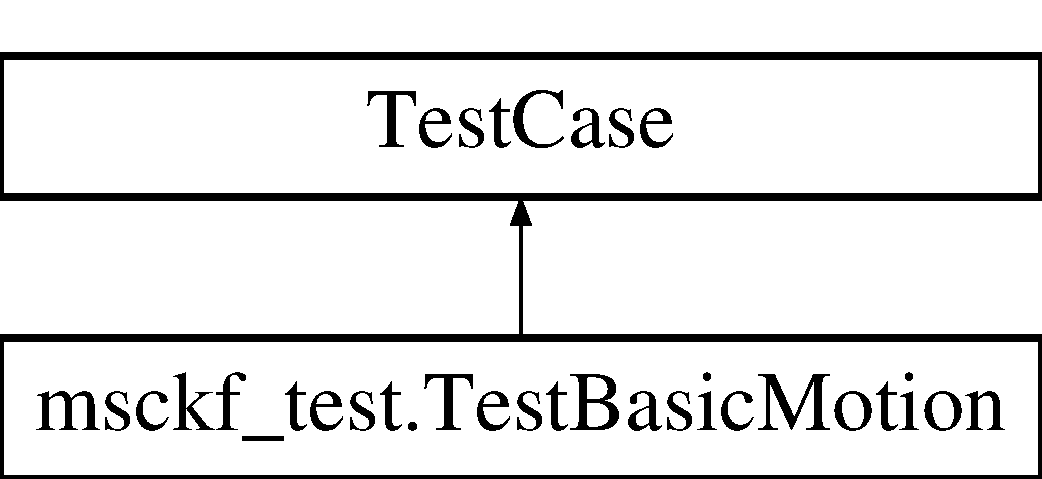
\includegraphics[height=2.000000cm]{classmsckf__test_1_1_test_basic_motion}
\end{center}
\end{figure}
\subsection*{Public Member Functions}
\begin{DoxyCompactItemize}
\item 
\hypertarget{classmsckf__test_1_1_test_basic_motion_a404257b0be26cb61f9a40c86c3ed9038}{def {\bfseries test\-\_\-no\-\_\-movement}}\label{classmsckf__test_1_1_test_basic_motion_a404257b0be26cb61f9a40c86c3ed9038}

\item 
\hypertarget{classmsckf__test_1_1_test_basic_motion_acef0d837aaee3cc362efeed06df5a5c2}{def {\bfseries test\-\_\-simple\-\_\-move\-\_\-in\-\_\-x\-\_\-direction}}\label{classmsckf__test_1_1_test_basic_motion_acef0d837aaee3cc362efeed06df5a5c2}

\item 
\hypertarget{classmsckf__test_1_1_test_basic_motion_a2efc71e9537bf2671bbe4174c57895b7}{def {\bfseries test\-\_\-simple\-\_\-rotation\-\_\-about\-\_\-x\-\_\-axis}}\label{classmsckf__test_1_1_test_basic_motion_a2efc71e9537bf2671bbe4174c57895b7}

\end{DoxyCompactItemize}


\subsection{Detailed Description}


Definition at line 81 of file msckf\-\_\-test.\-py.



The documentation for this class was generated from the following file\-:\begin{DoxyCompactItemize}
\item 
/home/travis/build/tomas789/tonav/prototype/msckf\-\_\-test.\-py\end{DoxyCompactItemize}

\hypertarget{classmsckf__test_1_1_test_frame_transformations}{\section{msckf\-\_\-test.\-Test\-Frame\-Transformations Class Reference}
\label{classmsckf__test_1_1_test_frame_transformations}\index{msckf\-\_\-test.\-Test\-Frame\-Transformations@{msckf\-\_\-test.\-Test\-Frame\-Transformations}}
}
Inheritance diagram for msckf\-\_\-test.\-Test\-Frame\-Transformations\-:\begin{figure}[H]
\begin{center}
\leavevmode
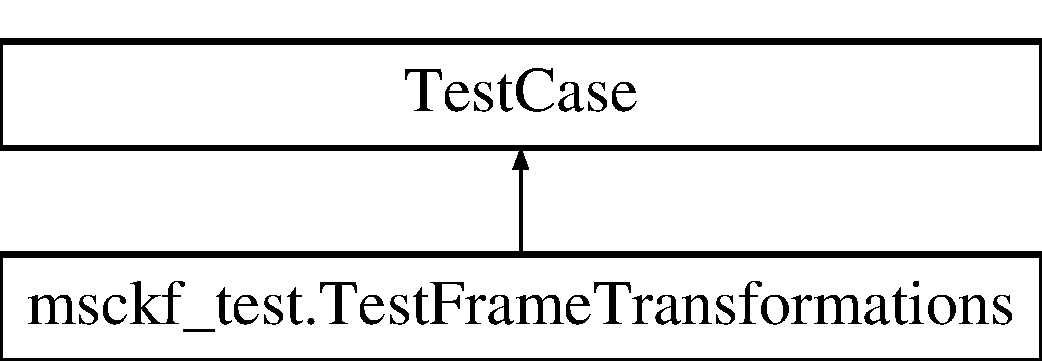
\includegraphics[height=2.000000cm]{classmsckf__test_1_1_test_frame_transformations}
\end{center}
\end{figure}
\subsection*{Public Member Functions}
\begin{DoxyCompactItemize}
\item 
\hypertarget{classmsckf__test_1_1_test_frame_transformations_a723d6acda4eab14e0388203fc4e9f206}{def {\bfseries test\-\_\-initial\-\_\-setup}}\label{classmsckf__test_1_1_test_frame_transformations_a723d6acda4eab14e0388203fc4e9f206}

\item 
\hypertarget{classmsckf__test_1_1_test_frame_transformations_a7ab5c8610b77c7aa5954705ff579aebe}{def {\bfseries test\-\_\-rotation\-\_\-of\-\_\-camera\-\_\-pose\-\_\-after\-\_\-rotation}}\label{classmsckf__test_1_1_test_frame_transformations_a7ab5c8610b77c7aa5954705ff579aebe}

\end{DoxyCompactItemize}


\subsection{Detailed Description}


Definition at line 120 of file msckf\-\_\-test.\-py.



The documentation for this class was generated from the following file\-:\begin{DoxyCompactItemize}
\item 
/home/travis/build/tomas789/tonav/prototype/msckf\-\_\-test.\-py\end{DoxyCompactItemize}

\hypertarget{classmsckf__test_1_1_test_numpy_quaternion}{\section{msckf\-\_\-test.\-Test\-Numpy\-Quaternion Class Reference}
\label{classmsckf__test_1_1_test_numpy_quaternion}\index{msckf\-\_\-test.\-Test\-Numpy\-Quaternion@{msckf\-\_\-test.\-Test\-Numpy\-Quaternion}}
}
Inheritance diagram for msckf\-\_\-test.\-Test\-Numpy\-Quaternion\-:\begin{figure}[H]
\begin{center}
\leavevmode
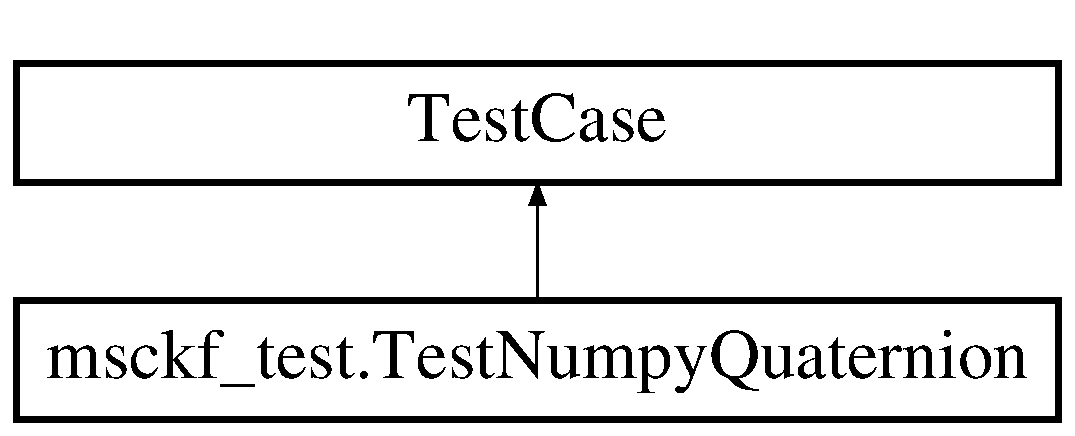
\includegraphics[height=2.000000cm]{classmsckf__test_1_1_test_numpy_quaternion}
\end{center}
\end{figure}
\subsection*{Public Member Functions}
\begin{DoxyCompactItemize}
\item 
\hypertarget{classmsckf__test_1_1_test_numpy_quaternion_ac120e1e04eb3df181bbe9c6b3ebac999}{def {\bfseries test\-\_\-multiply\-\_\-by\-\_\-unit\-\_\-quaternion}}\label{classmsckf__test_1_1_test_numpy_quaternion_ac120e1e04eb3df181bbe9c6b3ebac999}

\item 
\hypertarget{classmsckf__test_1_1_test_numpy_quaternion_a48568c2d3071f0c3aa8db91ae2fefdc8}{def {\bfseries test\-\_\-element\-\_\-order}}\label{classmsckf__test_1_1_test_numpy_quaternion_a48568c2d3071f0c3aa8db91ae2fefdc8}

\end{DoxyCompactItemize}


\subsection{Detailed Description}


Definition at line 8 of file msckf\-\_\-test.\-py.



The documentation for this class was generated from the following file\-:\begin{DoxyCompactItemize}
\item 
/home/travis/build/tomas789/tonav/prototype/msckf\-\_\-test.\-py\end{DoxyCompactItemize}

\hypertarget{classmsckf__test_1_1_test_quaternion_to_rotation_matrix}{\section{msckf\-\_\-test.\-Test\-Quaternion\-To\-Rotation\-Matrix Class Reference}
\label{classmsckf__test_1_1_test_quaternion_to_rotation_matrix}\index{msckf\-\_\-test.\-Test\-Quaternion\-To\-Rotation\-Matrix@{msckf\-\_\-test.\-Test\-Quaternion\-To\-Rotation\-Matrix}}
}
Inheritance diagram for msckf\-\_\-test.\-Test\-Quaternion\-To\-Rotation\-Matrix\-:\begin{figure}[H]
\begin{center}
\leavevmode
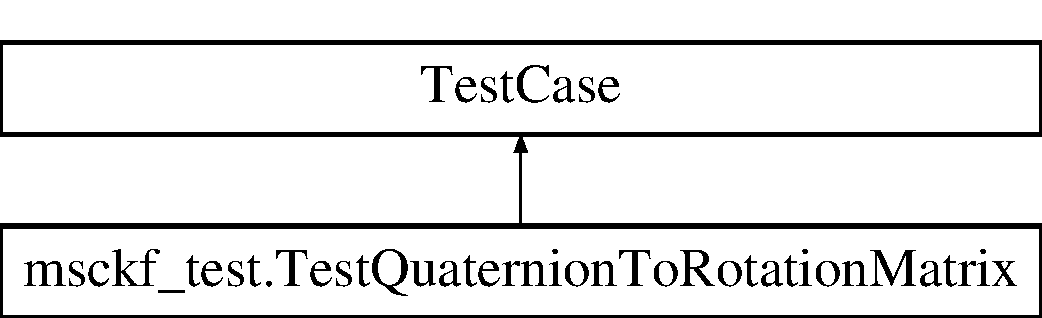
\includegraphics[height=2.000000cm]{classmsckf__test_1_1_test_quaternion_to_rotation_matrix}
\end{center}
\end{figure}
\subsection*{Public Member Functions}
\begin{DoxyCompactItemize}
\item 
\hypertarget{classmsckf__test_1_1_test_quaternion_to_rotation_matrix_a5ce323c18ba9e5cf9c2793796ef313a8}{def {\bfseries test\-\_\-unit\-\_\-quaternion\-\_\-is\-\_\-unit\-\_\-matrix}}\label{classmsckf__test_1_1_test_quaternion_to_rotation_matrix_a5ce323c18ba9e5cf9c2793796ef313a8}

\item 
\hypertarget{classmsckf__test_1_1_test_quaternion_to_rotation_matrix_ac776e17660756aeb2029a96d19710c02}{def {\bfseries test\-\_\-non\-\_\-unit\-\_\-quaternion\-\_\-is\-\_\-non\-\_\-unit\-\_\-matrix}}\label{classmsckf__test_1_1_test_quaternion_to_rotation_matrix_ac776e17660756aeb2029a96d19710c02}

\item 
\hypertarget{classmsckf__test_1_1_test_quaternion_to_rotation_matrix_adb1f5ec79fbb9273b661cbdbbf642c72}{def {\bfseries test\-\_\-rotation\-\_\-matrix\-\_\-of\-\_\-oposite\-\_\-quaternion\-\_\-is\-\_\-the\-\_\-same}}\label{classmsckf__test_1_1_test_quaternion_to_rotation_matrix_adb1f5ec79fbb9273b661cbdbbf642c72}

\item 
\hypertarget{classmsckf__test_1_1_test_quaternion_to_rotation_matrix_aa2d7002bb2a55d8b16e148d16cbc7c0f}{def {\bfseries test\-\_\-rotation\-\_\-matrix\-\_\-of\-\_\-conjugate\-\_\-quaternion\-\_\-is\-\_\-transposed\-\_\-rotation\-\_\-matrix}}\label{classmsckf__test_1_1_test_quaternion_to_rotation_matrix_aa2d7002bb2a55d8b16e148d16cbc7c0f}

\item 
\hypertarget{classmsckf__test_1_1_test_quaternion_to_rotation_matrix_ac52b74a18ab3ac86e31c18cfc8e05a66}{def {\bfseries test\-\_\-rotation\-\_\-matrix\-\_\-of\-\_\-composition\-\_\-is\-\_\-dot\-\_\-product\-\_\-of\-\_\-rotation\-\_\-matrices}}\label{classmsckf__test_1_1_test_quaternion_to_rotation_matrix_ac52b74a18ab3ac86e31c18cfc8e05a66}

\item 
\hypertarget{classmsckf__test_1_1_test_quaternion_to_rotation_matrix_aa7654932fddf9ceff835f95fa592d01d}{def {\bfseries vector\-\_\-to\-\_\-quaternion\-\_\-form\-\_\-and\-\_\-back\-\_\-is\-\_\-the\-\_\-same\-\_\-vector}}\label{classmsckf__test_1_1_test_quaternion_to_rotation_matrix_aa7654932fddf9ceff835f95fa592d01d}

\item 
\hypertarget{classmsckf__test_1_1_test_quaternion_to_rotation_matrix_a059360bc65644e9013dd18e7eb1ac16e}{def {\bfseries test\-\_\-transformation\-\_\-using\-\_\-sandwich\-\_\-and\-\_\-rotation\-\_\-matrix\-\_\-are\-\_\-same}}\label{classmsckf__test_1_1_test_quaternion_to_rotation_matrix_a059360bc65644e9013dd18e7eb1ac16e}

\end{DoxyCompactItemize}


\subsection{Detailed Description}


Definition at line 28 of file msckf\-\_\-test.\-py.



The documentation for this class was generated from the following file\-:\begin{DoxyCompactItemize}
\item 
/home/travis/build/tomas789/tonav/prototype/msckf\-\_\-test.\-py\end{DoxyCompactItemize}

\hypertarget{class_tonav}{\section{Tonav Class Reference}
\label{class_tonav}\index{Tonav@{Tonav}}
}


This is main class for communicating with filter. You can pass I\-M\-U and camera data to filter through it and get information about current filter state.  




{\ttfamily \#include $<$tonav.\-h$>$}

\subsection*{Public Member Functions}
\begin{DoxyCompactItemize}
\item 
\hyperlink{class_tonav_a0c3d527cc8ec6832d4ea650ad31c726a}{Tonav} (\hyperlink{class_calibration}{Calibration} \&calibration)
\begin{DoxyCompactList}\small\item\em Initialize filter with configuration. \end{DoxyCompactList}\item 
void \hyperlink{class_tonav_ac458c8712b1eeef1ba169835706d26fd}{update\-Acceleration} (double time, Eigen\-::\-Vector3d accel)
\begin{DoxyCompactList}\small\item\em Perform navigation step with data from accelerometer. \end{DoxyCompactList}\item 
void \hyperlink{class_tonav_a02a596cd5acf1799830499dd97e5e2e5}{update\-Rotation\-Rate} (double time, Eigen\-::\-Vector3d gyro)
\begin{DoxyCompactList}\small\item\em Perform navigation step with data from gyroscope. \end{DoxyCompactList}\item 
void \hyperlink{class_tonav_ac7c7cdaa16941df03aca92a3eaa75ed7}{update\-Acceleration\-And\-Rotation\-Rate} (double time, Eigen\-::\-Vector3d accel, Eigen\-::\-Vector3d gyro)
\begin{DoxyCompactList}\small\item\em Perform navigation step with data from both accelerometer and gyroscore. \end{DoxyCompactList}\item 
void \hyperlink{class_tonav_a765f593b621a40052a01b7d0449d9b8e}{update\-Image} (double time, cv\-::\-Mat \&image)
\begin{DoxyCompactList}\small\item\em Perform navigation step with image from camera. \end{DoxyCompactList}\item 
void \hyperlink{class_tonav_a53fddfad248ab9a75906e310266e1f0d}{set\-Camera\-Model\-Params} (const Eigen\-::\-Matrix3d \&camera\-\_\-matrix, const Eigen\-::\-Matrix$<$ double, 5, 1 $>$ distortion\-\_\-params)
\begin{DoxyCompactList}\small\item\em Set camera model params. \end{DoxyCompactList}\item 
\hypertarget{class_tonav_a6cd97922b947734bca02119a60135c30}{bool {\bfseries filter\-Was\-Updated} () const }\label{class_tonav_a6cd97922b947734bca02119a60135c30}

\item 
\hypertarget{class_tonav_a724c0d36fb1f182023831f70fa166e55}{Eigen\-::\-Quaterniond {\bfseries get\-Current\-Orientation} ()}\label{class_tonav_a724c0d36fb1f182023831f70fa166e55}

\item 
\hypertarget{class_tonav_a4717848cb42b3311e19d656de940bc65}{Eigen\-::\-Vector3d {\bfseries get\-Current\-Position} ()}\label{class_tonav_a4717848cb42b3311e19d656de940bc65}

\item 
\hypertarget{class_tonav_a3929b594397489b232e77e4344c8675a}{cv\-::\-Mat {\bfseries get\-Current\-Image} () const }\label{class_tonav_a3929b594397489b232e77e4344c8675a}

\end{DoxyCompactItemize}


\subsection{Detailed Description}
This is main class for communicating with filter. You can pass I\-M\-U and camera data to filter through it and get information about current filter state. 

As a user, you should only communicate with this class. 

Definition at line 19 of file tonav.\-h.



\subsection{Constructor \& Destructor Documentation}
\hypertarget{class_tonav_a0c3d527cc8ec6832d4ea650ad31c726a}{\index{Tonav@{Tonav}!Tonav@{Tonav}}
\index{Tonav@{Tonav}!Tonav@{Tonav}}
\subsubsection[{Tonav}]{\setlength{\rightskip}{0pt plus 5cm}Tonav\-::\-Tonav (
\begin{DoxyParamCaption}
\item[{{\bf Calibration} \&}]{calibration}
\end{DoxyParamCaption}
)}}\label{class_tonav_a0c3d527cc8ec6832d4ea650ad31c726a}


Initialize filter with configuration. 


\begin{DoxyParams}{Parameters}
{\em calibration} & \hyperlink{class_calibration}{Calibration} \\
\hline
\end{DoxyParams}


Definition at line 7 of file tonav.\-cpp.



\subsection{Member Function Documentation}
\hypertarget{class_tonav_a53fddfad248ab9a75906e310266e1f0d}{\index{Tonav@{Tonav}!set\-Camera\-Model\-Params@{set\-Camera\-Model\-Params}}
\index{set\-Camera\-Model\-Params@{set\-Camera\-Model\-Params}!Tonav@{Tonav}}
\subsubsection[{set\-Camera\-Model\-Params}]{\setlength{\rightskip}{0pt plus 5cm}void Tonav\-::set\-Camera\-Model\-Params (
\begin{DoxyParamCaption}
\item[{const Eigen\-::\-Matrix3d \&}]{camera\-\_\-matrix, }
\item[{const Eigen\-::\-Matrix$<$ double, 5, 1 $>$}]{distortion\-\_\-params}
\end{DoxyParamCaption}
)}}\label{class_tonav_a53fddfad248ab9a75906e310266e1f0d}


Set camera model params. 

\hyperlink{class_tonav}{Tonav} is using pinhole camera modes as implemented in Open\-C\-V. Using this function, you can set camera intrinsics parameters.

Camera matrix\-:

$ \begin{pmatrix} f_x & 0 & c_x \\ 0 & f_y & c_y \\ 0 & 0 & 1 \end{pmatrix} $

Distortion params\-:

$ \begin{pmatrix} k_1 & k_2 & p_1 & p_2 & k_3 \end{pmatrix} $


\begin{DoxyParams}{Parameters}
{\em camera\-\_\-matrix} & Camera matrix \\
\hline
{\em distortion\-\_\-params} & Distortion parameters \\
\hline
\end{DoxyParams}
\hypertarget{class_tonav_ac458c8712b1eeef1ba169835706d26fd}{\index{Tonav@{Tonav}!update\-Acceleration@{update\-Acceleration}}
\index{update\-Acceleration@{update\-Acceleration}!Tonav@{Tonav}}
\subsubsection[{update\-Acceleration}]{\setlength{\rightskip}{0pt plus 5cm}void Tonav\-::update\-Acceleration (
\begin{DoxyParamCaption}
\item[{double}]{time, }
\item[{Eigen\-::\-Vector3d}]{accel}
\end{DoxyParamCaption}
)}}\label{class_tonav_ac458c8712b1eeef1ba169835706d26fd}


Perform navigation step with data from accelerometer. 

Parameter {\ttfamily accel} is vector $(x, y, z)$ measured in $\frac{m}{s^2}$.


\begin{DoxyParams}{Parameters}
{\em time} & Time at which accelerometer data were captured. \\
\hline
{\em accel} & 3\-D vector of accelerometer data. \\
\hline
\end{DoxyParams}


Definition at line 13 of file tonav.\-cpp.

\hypertarget{class_tonav_ac7c7cdaa16941df03aca92a3eaa75ed7}{\index{Tonav@{Tonav}!update\-Acceleration\-And\-Rotation\-Rate@{update\-Acceleration\-And\-Rotation\-Rate}}
\index{update\-Acceleration\-And\-Rotation\-Rate@{update\-Acceleration\-And\-Rotation\-Rate}!Tonav@{Tonav}}
\subsubsection[{update\-Acceleration\-And\-Rotation\-Rate}]{\setlength{\rightskip}{0pt plus 5cm}void Tonav\-::update\-Acceleration\-And\-Rotation\-Rate (
\begin{DoxyParamCaption}
\item[{double}]{time, }
\item[{Eigen\-::\-Vector3d}]{accel, }
\item[{Eigen\-::\-Vector3d}]{gyro}
\end{DoxyParamCaption}
)}}\label{class_tonav_ac7c7cdaa16941df03aca92a3eaa75ed7}


Perform navigation step with data from both accelerometer and gyroscore. 

Parameter {\ttfamily accel} is vector $(x, y, z)$ measured in $\frac{m}{s^2}$. Parameter {\ttfamily gyro} is vector $(x, y, z)$ measured in $\frac{rad}{s}$.


\begin{DoxyParams}{Parameters}
{\em time} & Time at which accelerometer and gyroscope data were both captured. \\
\hline
{\em accel} & 3\-D vector of accelerometer data. \\
\hline
{\em gyro} & 3\-D vector of gyroscope data. \\
\hline
\end{DoxyParams}


Definition at line 23 of file tonav.\-cpp.

\hypertarget{class_tonav_a765f593b621a40052a01b7d0449d9b8e}{\index{Tonav@{Tonav}!update\-Image@{update\-Image}}
\index{update\-Image@{update\-Image}!Tonav@{Tonav}}
\subsubsection[{update\-Image}]{\setlength{\rightskip}{0pt plus 5cm}void Tonav\-::update\-Image (
\begin{DoxyParamCaption}
\item[{double}]{time, }
\item[{cv\-::\-Mat \&}]{image}
\end{DoxyParamCaption}
)}}\label{class_tonav_a765f593b621a40052a01b7d0449d9b8e}


Perform navigation step with image from camera. 

Time passed to this function should be as deterministic as possible. Try to avoid as much buffering as you can. Also don't do any variable-\/duration image processing like detecting features from image.

Image should by in format G\-R\-A\-Y8 and should have reasonable resolution. Full-\/\-H\-D is unnecessarily large. Something about 640x480 is good enough. It speeds up processing of the image and delivers more real-\/time localization.


\begin{DoxyParams}{Parameters}
{\em time} & Time at which camera image was captured. \\
\hline
{\em image} & Captured image. \\
\hline
\end{DoxyParams}


Definition at line 29 of file tonav.\-cpp.

\hypertarget{class_tonav_a02a596cd5acf1799830499dd97e5e2e5}{\index{Tonav@{Tonav}!update\-Rotation\-Rate@{update\-Rotation\-Rate}}
\index{update\-Rotation\-Rate@{update\-Rotation\-Rate}!Tonav@{Tonav}}
\subsubsection[{update\-Rotation\-Rate}]{\setlength{\rightskip}{0pt plus 5cm}void Tonav\-::update\-Rotation\-Rate (
\begin{DoxyParamCaption}
\item[{double}]{time, }
\item[{Eigen\-::\-Vector3d}]{gyro}
\end{DoxyParamCaption}
)}}\label{class_tonav_a02a596cd5acf1799830499dd97e5e2e5}


Perform navigation step with data from gyroscope. 

Parameter {\ttfamily gyro} is vector $(x, y, z)$ measured in $\frac{rad}{s}$.


\begin{DoxyParams}{Parameters}
{\em time} & Time at which gyroscope data were captured. \\
\hline
{\em gyro} & 3\-D vector of gyroscope data. \\
\hline
\end{DoxyParams}


Definition at line 18 of file tonav.\-cpp.



The documentation for this class was generated from the following files\-:\begin{DoxyCompactItemize}
\item 
/home/tomaskrejci/catkin\-\_\-ws/src/tonav/include/tonav.\-h\item 
/home/tomaskrejci/catkin\-\_\-ws/src/tonav/src/tonav.\-cpp\end{DoxyCompactItemize}

\hypertarget{class_tonav_ros}{\section{Tonav\-Ros Class Reference}
\label{class_tonav_ros}\index{Tonav\-Ros@{Tonav\-Ros}}
}


\hyperlink{class_tonav}{Tonav} navigation node for R\-O\-S.  




{\ttfamily \#include $<$tonav\-\_\-ros.\-h$>$}

\subsection*{Public Member Functions}
\begin{DoxyCompactItemize}
\item 
int \hyperlink{class_tonav_ros_aa64cf50545f6cf41c538679703809724}{run} (int argc, char $\ast$argv\mbox{[}$\,$\mbox{]})
\begin{DoxyCompactList}\small\item\em Run navigation node. \end{DoxyCompactList}\end{DoxyCompactItemize}


\subsection{Detailed Description}
\hyperlink{class_tonav}{Tonav} navigation node for R\-O\-S. 

This is full implementation of R\-O\-S node performing navigation using data directly from R\-O\-S. It also publishes result to R\-O\-S. 

Definition at line 23 of file tonav\-\_\-ros.\-h.



\subsection{Member Function Documentation}
\hypertarget{class_tonav_ros_aa64cf50545f6cf41c538679703809724}{\index{Tonav\-Ros@{Tonav\-Ros}!run@{run}}
\index{run@{run}!TonavRos@{Tonav\-Ros}}
\subsubsection[{run}]{\setlength{\rightskip}{0pt plus 5cm}int Tonav\-Ros\-::run (
\begin{DoxyParamCaption}
\item[{int}]{argc, }
\item[{char $\ast$}]{argv\mbox{[}$\,$\mbox{]}}
\end{DoxyParamCaption}
)}}\label{class_tonav_ros_aa64cf50545f6cf41c538679703809724}


Run navigation node. 

Run R\-O\-S node and start navigation. This is blocking function. It also calls {\ttfamily ros\-::init} function.


\begin{DoxyParams}{Parameters}
{\em argc} & Number of command line arguments. \\
\hline
{\em argv} & List of command line arguments. \\
\hline
\end{DoxyParams}


Definition at line 20 of file tonav\-\_\-ros.\-cpp.



The documentation for this class was generated from the following files\-:\begin{DoxyCompactItemize}
\item 
/home/tomaskrejci/catkin\-\_\-ws/src/tonav/include/tonav\-\_\-ros.\-h\item 
/home/tomaskrejci/catkin\-\_\-ws/src/tonav/src/tonav\-\_\-ros.\-cpp\end{DoxyCompactItemize}

\hypertarget{classimage__transport_1_1_transport_hints}{\section{image\-\_\-transport\-:\-:Transport\-Hints Class Reference}
\label{classimage__transport_1_1_transport_hints}\index{image\-\_\-transport\-::\-Transport\-Hints@{image\-\_\-transport\-::\-Transport\-Hints}}
}


Stores transport settings for an image topic subscription.  




{\ttfamily \#include $<$transport\-\_\-hints.\-h$>$}

\subsection*{Public Member Functions}
\begin{DoxyCompactItemize}
\item 
\hyperlink{classimage__transport_1_1_transport_hints_a1685aa1484249c2a4f70d91a2eac470a}{Transport\-Hints} (const std\-::string \&default\-\_\-transport=\char`\"{}raw\char`\"{}, const ros\-::\-Transport\-Hints \&ros\-\_\-hints=ros\-::\-Transport\-Hints(), const ros\-::\-Node\-Handle \&parameter\-\_\-nh=ros\-::\-Node\-Handle(\char`\"{}$\sim$\char`\"{}), const std\-::string \&parameter\-\_\-name=\char`\"{}image\-\_\-transport\char`\"{})
\begin{DoxyCompactList}\small\item\em Constructor. \end{DoxyCompactList}\item 
\hypertarget{classimage__transport_1_1_transport_hints_a03ac9b94b5d821ad58069de46750429f}{const std\-::string \& {\bfseries get\-Transport} () const }\label{classimage__transport_1_1_transport_hints_a03ac9b94b5d821ad58069de46750429f}

\item 
\hypertarget{classimage__transport_1_1_transport_hints_a69b2353e24790b8e3e25aaa5b7c2ae2c}{const ros\-::\-Transport\-Hints \& {\bfseries get\-Ros\-Hints} () const }\label{classimage__transport_1_1_transport_hints_a69b2353e24790b8e3e25aaa5b7c2ae2c}

\item 
\hypertarget{classimage__transport_1_1_transport_hints_a6f4f312029db188135e83edd7508cfbd}{const ros\-::\-Node\-Handle \& {\bfseries get\-Parameter\-N\-H} () const }\label{classimage__transport_1_1_transport_hints_a6f4f312029db188135e83edd7508cfbd}

\end{DoxyCompactItemize}


\subsection{Detailed Description}
Stores transport settings for an image topic subscription. 

Definition at line 45 of file transport\-\_\-hints.\-h.



\subsection{Constructor \& Destructor Documentation}
\hypertarget{classimage__transport_1_1_transport_hints_a1685aa1484249c2a4f70d91a2eac470a}{\index{image\-\_\-transport\-::\-Transport\-Hints@{image\-\_\-transport\-::\-Transport\-Hints}!Transport\-Hints@{Transport\-Hints}}
\index{Transport\-Hints@{Transport\-Hints}!image_transport::TransportHints@{image\-\_\-transport\-::\-Transport\-Hints}}
\subsubsection[{Transport\-Hints}]{\setlength{\rightskip}{0pt plus 5cm}image\-\_\-transport\-::\-Transport\-Hints\-::\-Transport\-Hints (
\begin{DoxyParamCaption}
\item[{const std\-::string \&}]{default\-\_\-transport = {\ttfamily \char`\"{}raw\char`\"{}}, }
\item[{const ros\-::\-Transport\-Hints \&}]{ros\-\_\-hints = {\ttfamily ros\-:\-:TransportHints()}, }
\item[{const ros\-::\-Node\-Handle \&}]{parameter\-\_\-nh = {\ttfamily ros\-:\-:NodeHandle(\char`\"{}$\sim$\char`\"{})}, }
\item[{const std\-::string \&}]{parameter\-\_\-name = {\ttfamily \char`\"{}image\-\_\-transport\char`\"{}}}
\end{DoxyParamCaption}
)\hspace{0.3cm}{\ttfamily [inline]}}}\label{classimage__transport_1_1_transport_hints_a1685aa1484249c2a4f70d91a2eac470a}


Constructor. 

The default transport can be overridden by setting a certain parameter to the name of the desired transport. By default this parameter is named \char`\"{}image\-\_\-transport\char`\"{} in the node's local namespace. For consistency across R\-O\-S applications, the name of this parameter should not be changed without good reason.


\begin{DoxyParams}{Parameters}
{\em default\-\_\-transport} & Preferred transport to use \\
\hline
{\em ros\-\_\-hints} & Hints to pass through to R\-O\-S subscriptions \\
\hline
{\em parameter\-\_\-nh} & Node handle to use when looking up the transport parameter. Defaults to the local namespace. \\
\hline
{\em parameter\-\_\-name} & The name of the transport parameter \\
\hline
\end{DoxyParams}


Definition at line 62 of file transport\-\_\-hints.\-h.



The documentation for this class was generated from the following file\-:\begin{DoxyCompactItemize}
\item 
/home/travis/catkin\-\_\-ws/src/image\-\_\-common/image\-\_\-transport/include/image\-\_\-transport/transport\-\_\-hints.\-h\end{DoxyCompactItemize}

\hypertarget{classimage__transport_1_1_transport_load_exception}{\section{image\-\_\-transport\-:\-:Transport\-Load\-Exception Class Reference}
\label{classimage__transport_1_1_transport_load_exception}\index{image\-\_\-transport\-::\-Transport\-Load\-Exception@{image\-\_\-transport\-::\-Transport\-Load\-Exception}}
}


An exception class thrown when image\-\_\-transport is unable to load a requested transport.  




{\ttfamily \#include $<$exception.\-h$>$}

Inheritance diagram for image\-\_\-transport\-:\-:Transport\-Load\-Exception\-:\begin{figure}[H]
\begin{center}
\leavevmode
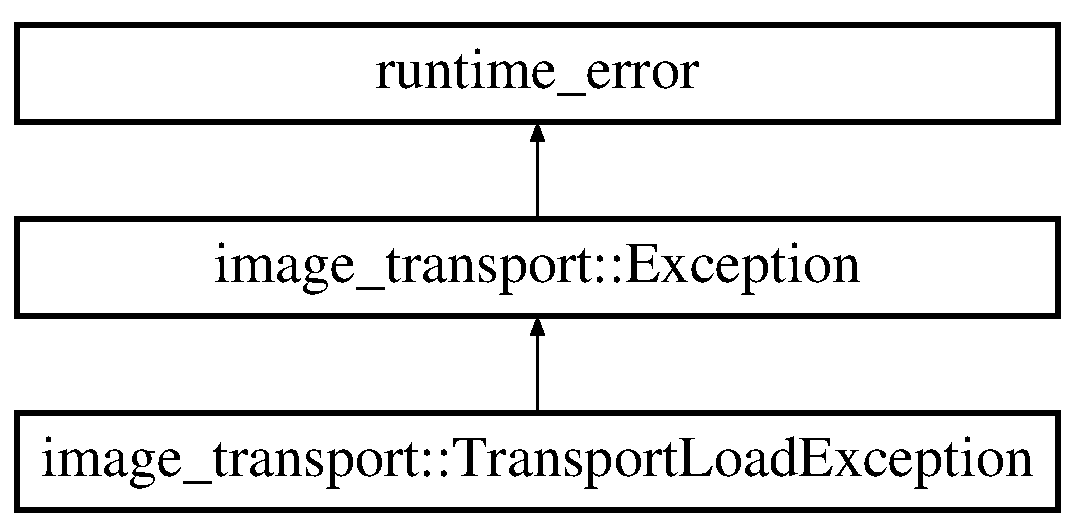
\includegraphics[height=3.000000cm]{classimage__transport_1_1_transport_load_exception}
\end{center}
\end{figure}
\subsection*{Public Member Functions}
\begin{DoxyCompactItemize}
\item 
\hypertarget{classimage__transport_1_1_transport_load_exception_ae57f655548bd6acdc0a63667232a3ba8}{{\bfseries Transport\-Load\-Exception} (const std\-::string \&transport, const std\-::string \&message)}\label{classimage__transport_1_1_transport_load_exception_ae57f655548bd6acdc0a63667232a3ba8}

\item 
\hypertarget{classimage__transport_1_1_transport_load_exception_a6c79ac8f03b55513812e40f26e39e1d6}{std\-::string {\bfseries get\-Transport} () const }\label{classimage__transport_1_1_transport_load_exception_a6c79ac8f03b55513812e40f26e39e1d6}

\end{DoxyCompactItemize}
\subsection*{Protected Attributes}
\begin{DoxyCompactItemize}
\item 
\hypertarget{classimage__transport_1_1_transport_load_exception_a0f852f96a21f41580f0c4848247289ae}{const char $\ast$ {\bfseries transport\-\_\-}}\label{classimage__transport_1_1_transport_load_exception_a0f852f96a21f41580f0c4848247289ae}

\end{DoxyCompactItemize}


\subsection{Detailed Description}
An exception class thrown when image\-\_\-transport is unable to load a requested transport. 

Definition at line 54 of file exception.\-h.



The documentation for this class was generated from the following file\-:\begin{DoxyCompactItemize}
\item 
/home/travis/catkin\-\_\-ws/src/image\-\_\-common/image\-\_\-transport/include/image\-\_\-transport/exception.\-h\end{DoxyCompactItemize}

%--- End generated contents ---

% Index
\newpage
\phantomsection
\addcontentsline{toc}{chapter}{Index}
\printindex

\end{document}
